% !TeX encoding = utf-8
% !TeX program = pdflatex

% !Mode:: "TeX:UTF-8"
%%  本模板可以使用以下两种方式编译:
%%
%%     1. PDFLaTeX[推荐]
%%     2. XeLaTeX

%%  注意:
%%   1. 文件默认的编码为 UTF-8 对于windows,请选用支持UTF-8编码的编辑器。
%%   2. 若是模板有什么问题,请及时与我们取得联系,Email:latexstudio@qq.com。  



\documentclass{swmcmthesis}

\usepackage{indentfirst} % 确保章节的第一段也会缩进
\setlength{\parindent}{1.5em} 
\usepackage{amsmath}
\usepackage{amssymb}
\usepackage{mathtools}
\usepackage{float}
\usepackage{subcaption}

%%%%%%%%%%%%填写相关信息%%%%%%%%%%%%%%%%%%%%%%%%%%
\title{Revolutionizing Spatial Data Analysis through \\ Collaborative Kriging Innovations} %论文题目

\baominghao{2024082728930}           %报名号,修改为自己的队号

\zubie{B} %选题

\abstract{ 
This study explores collaborative estimation methods for spatial variables to improve spatial analysis precision. It incorporates traditional geostatistical techniques, such as \textbf{Kriging interpolation}, along with modern machine learning algorithms like SVM. We examine the impact of collaborative variables on target predictions, leading to more accurate spatial models. Furthermore, a comprehensive comparison of prediction methods provides practical and theoretical insights for optimizing spatial prediction.

\textbf{For Problem 1}, we apply the \textbf{Kriging interpolation} method to predict unknown spatial attributes using a limited number of known data points. By varying the sample size, we evaluate the impact of sample scale on prediction accuracy, generating error maps and contour plots to visually analyze the relationship between sample size and estimation precision.

\textbf{For Problem 2}, through statistical analysis, we examine the relationship between the target variable and collaborative variables. Initially, \textbf{QQ-Plots} are used to determine the data distribution and show that Pearson correlation analysis might not be suitable. Subsequently, \textbf{Spearman's correlation coefficient} and \textbf{2D-KDE} methods are employed to identify the two collaborative variables most strongly associated with the target variable, which are variable 1 with a Spearman coefficient \textbf{value 0.75} and variable 4 with a Spearman coefficient \textbf{value 0.31}.

\textbf{For Problem 3}, we incorporate the two collaborative variables most strongly associated with the target variable (identified in Problem 2) into the spatial prediction models. The analysis utilizes \textbf{Co-Kriging}, \textbf{Support Vector Machines (SVM)}, and \textbf{Regression Kriging} methods. The cKDTree Algorithm is used to accelerate computing efficiency. Comparative analysis reveals that \textbf{Co-Kriging} demonstrates superior performance in reducing errors, while \textbf{Regression Kriging} also shows competitive advantages in certain scenarios. Both methods significantly outperformed traditional machine learning approaches, improving prediction accuracy.

\textbf{For Problem 4}, a superior \textbf{Co-Kriging} method (identified in Problem 3) is applied to predict the spatial distribution of data in Attachment 2. The contouring map result is shown in \textbf{Figure 18}. 

This study underscored the potential of combining geostatistical methods with collaborative estimation techniques in spatial data analysis. The findings provide valuable references for improving spatial prediction methods and highlight the importance of collaborative estimation approaches in enhancing prediction accuracy and reliability.} % 摘要

\keywords{Spatial Variable Estimation, Collaborative Estimation, Kriging, cKDTree, SVM}

\date{2024}

\begin{document}

% 生成首页
\maketitle
% 目录
\tableofcontents

\newpage

% -------------------------正文开始
%\setcounter{page}{1}
\section{Introduction}
\subsection{Problem Background}
In spatial data analysis, accurately predicting the distribution of spatial attributes is a significant challenge, especially when the data is sparse and difficult to collect. Unlike traditional statistics, this field assumes that data points are not independent but are spatially correlated, displaying trends across the entire landscape. This assumption forms the basis for advanced geostatistical methods such as Kriging and Co-Kriging, which are widely used in fields like environmental science, mining, and urban planning. These techniques are essential for making predictions at unsampled locations, helping to inform decision-making processes. However, implementing these techniques involves complex challenges, such as calculating the cross-covariance or cross-variogram functions between spatial variables, making these practical applications more challenging. Additionally, the integration of machine learning and other artificial intelligence techniques into spatial data analysis has introduced new methodologies that aim to improve efficiency and provide innovative solutions to longstanding spatial estimation problems. These modern approaches encourage the integration of traditional geostatistical techniques with advanced computational algorithms, aiming to produce more reliable predictions and effectively manage challenges related to variable sampling density and associated costs. This paper aims to study the collaborative estimation of spatial attributes under given data using specific methods.
\subsection{Restatement of the Problem}
\begin{itemize}
    \item \textbf{Question 1:} 
    Research how to infer the attribute values of unknown points in an entire area based on known spatial data points. This involves using statistical methods, such as Kriging interpolation, to predict the spatial attributes of unsampled points and analyze the impact of sample size changes on prediction results.
    
    \item \textbf{Question 2:} 
    Explore and analyze the relationship between the target variable and collaborative variables, assessing how their interactions affect the spatial distribution of the target variable. Select two variables that may have a stronger correlation with the target variable.
    
    \item \textbf{Question 3:} 
    Incorporate collaborative variables into spatial predictions to enhance accuracy by selecting the most relevant variables and applying multivariate statistical methods, such as Co-Kriging, to generate more accurate predictions of the spatial data distribution
    
    \item \textbf{Question 4:} 
    Address the challenge of insufficient data sampling by selecting and implementing the most suitable statistical method to predict missing spatial data. Based on the analysis results of the previous questions, identify the optimal method for addressing regions with sparse data and ensuring accurate and dependable prediction outcomes.
\end{itemize}

\subsection{Literature Review}
Borregaard et al. in their entry in the \textit{Encyclopedia of Ecology} discuss in detail the concepts and ecological applications of spatial distribution, providing us with a fundamental understanding of the topic \cite{bib6}. Oliver and Webster's article offers a detailed tutorial on Kriging computations and modeling, explaining key concepts such as variograms and Kriging predictions \cite{bib5}. This provides practical guidance for our team, aiding in the understanding and implementation of the Kriging method. The Laerd Statistics website and Minitab support page offer guidance on Spearman's rank correlation coefficient and Pearson correlation coefficient respectively \cite{bib2, bib3}. These resources are invaluable for understanding when to use these statistical methods and under what conditions they are applicable. The research by Du et al. and Erten et al. explores the cutting-edge advancements in the application of machine learning methods combined with Kriging techniques for spatial data handling \cite{bib8, bib9}. These studies demonstrate how machine learning can enhance the capabilities of traditional geostatistical methods, especially in the spatial prediction of geological attributes. These two articles provide us with new perspectives, especially in deciding to reapproach the problem using machine learning methods.


\subsection{Problem Analysis \& Our Work}
\begin{itemize}
    \item \textbf{Question 1:}  
    We use Kriging interpolation to estimate the spatial attributes at unsampled locations based on known data points. Our approach examines the impact of varying sample sizes and employs contour mapping for visual validation, ensuring that the interpolation method accurately reflects spatial continuity, as shown in the workflow diagram.
    
    \item \textbf{Question 2:} 
    The analysis of the relationship between the target and collaborative variables informs the enhancement of spatial distribution models. By utilizing cross-variograms and cross-covariance statistics, we identify and integrate two variables strongly correlated with the target into the modeling process. This enhances our prediction models, aligning them with the interdependencies shown in the workflow chart.
    
    \item \textbf{Question 3:}  
    Building on previous insights, we enhance the spatial prediction models through the integration of collaborative variables using Co-Kriging. This method leverages multivariate relationships to improve prediction accuracy, while we assess machine learning models and Regression Kriging for their potential to further improve the predictions, ensuring that these enhancements align with the procedural logic of the workflow chart.
    
    \item \textbf{Question 4:}  
    To overcome challenges in data-sparse regions, we select and apply the most effective statistical methods based on comprehensive evaluations of previous results. The chosen approach emphasizes ensuring prediction reliability under limited data scenarios, focusing on applying robust methods that integrate seamlessly with the strategic steps outlined in the workflow diagram.
\end{itemize}

\begin{figure}[h!t]
	\centering
	\begin{minipage}[t]{0.4\textwidth}
		\centering
		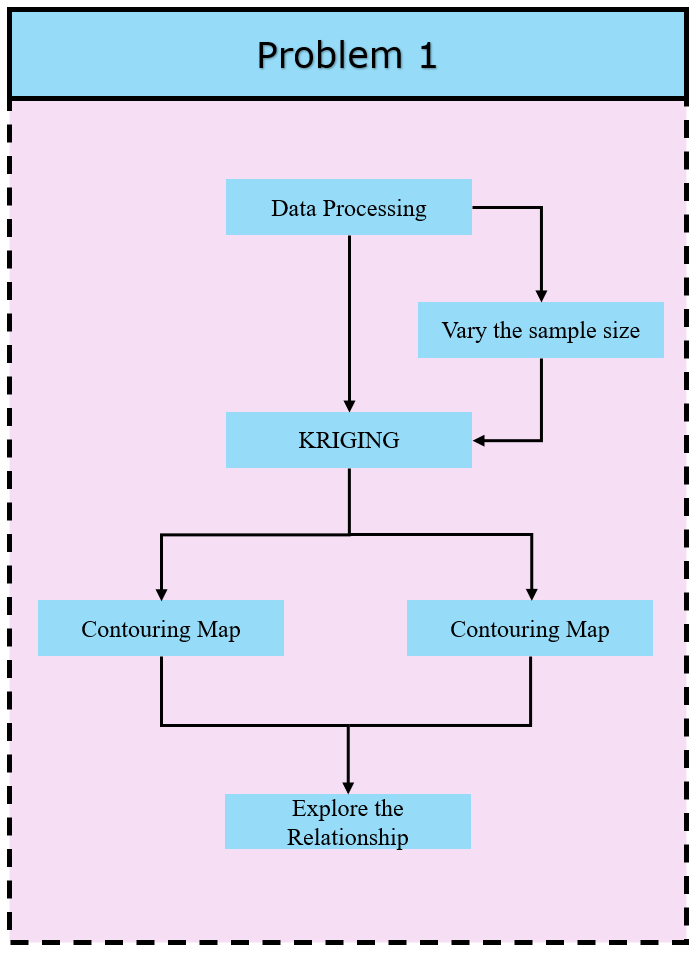
\includegraphics[width=\textwidth]{Problem 1.png}
		\caption{Problem 1 Flow Chart}
	\end{minipage}
	\hfill
	\begin{minipage}[t]{0.4\textwidth}
		\centering
		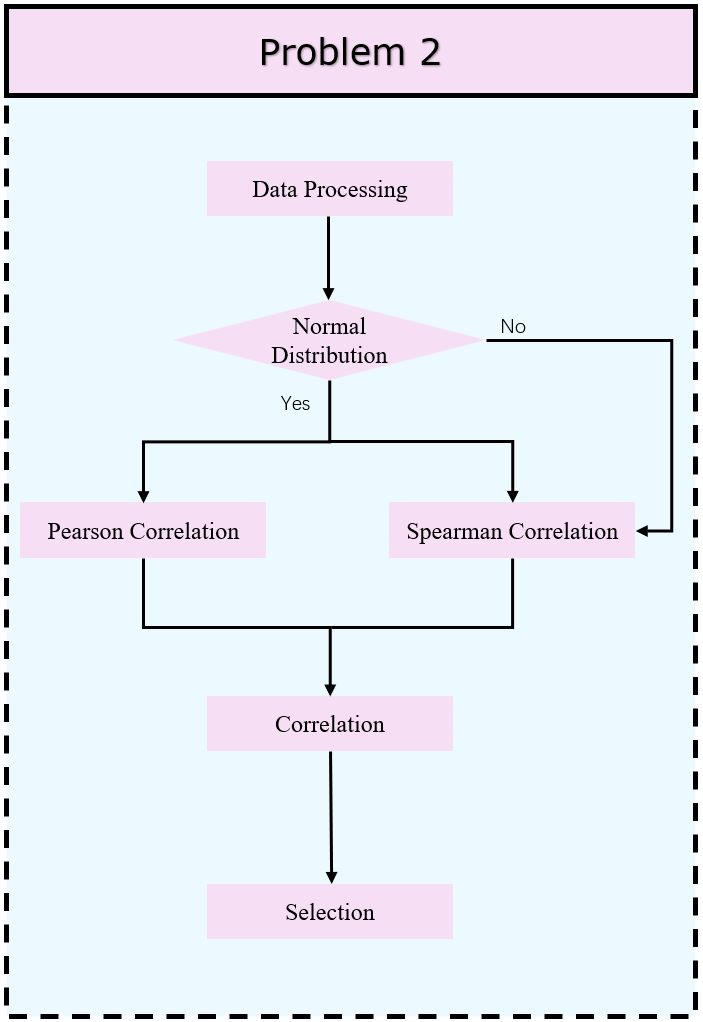
\includegraphics[width=\textwidth]{Problem 2.png}
		\caption{Problem 2 Flow Chart}
	\end{minipage}
\end{figure}

\begin{figure}[h!t]
	\centering
	\begin{minipage}[t]{0.5\textwidth}
		\centering
		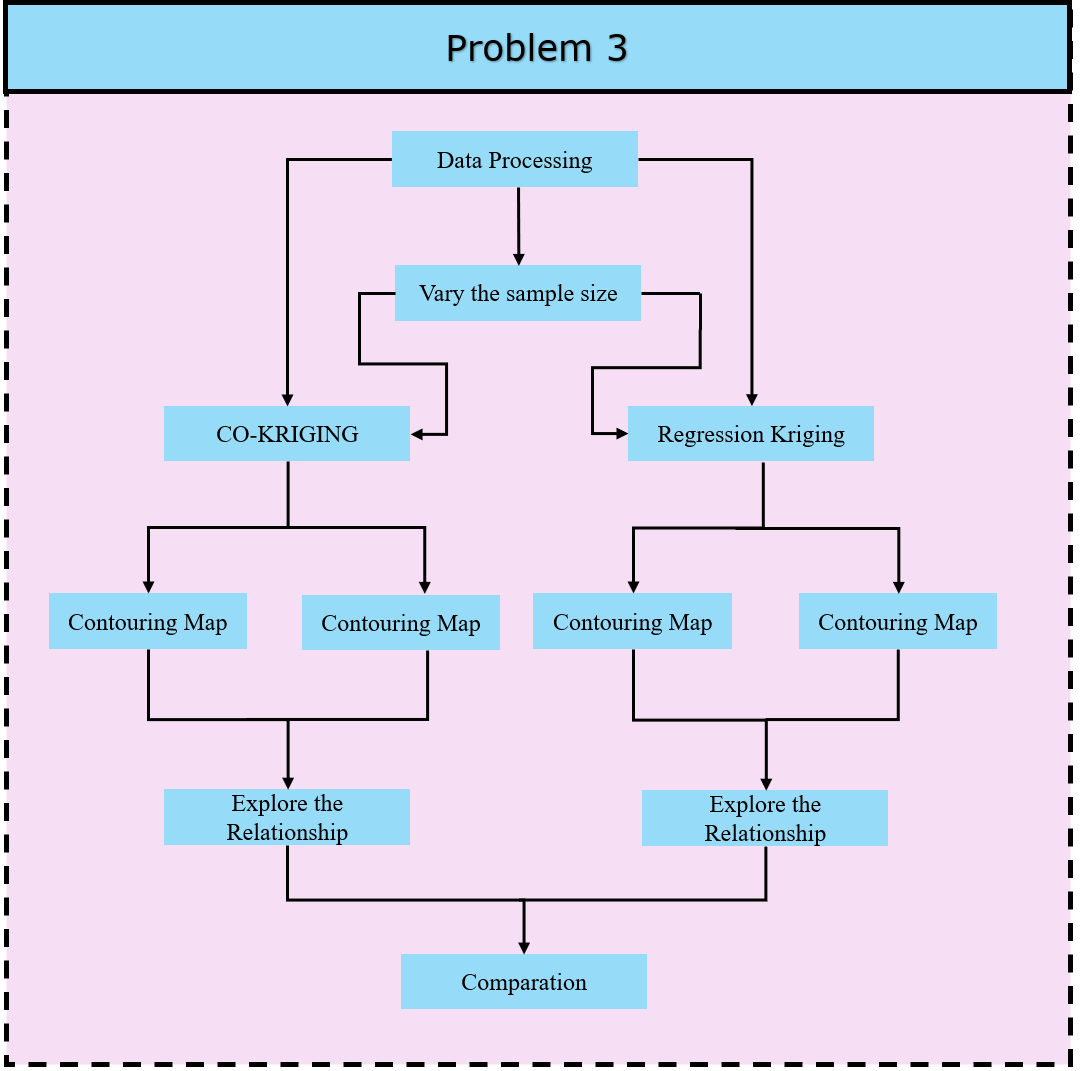
\includegraphics[width=\textwidth]{Problem 3.png}
		\caption{Problem 3 Flow Chart}
	\end{minipage}
	\hfill
	\begin{minipage}[t]{0.4\textwidth}
		\centering
		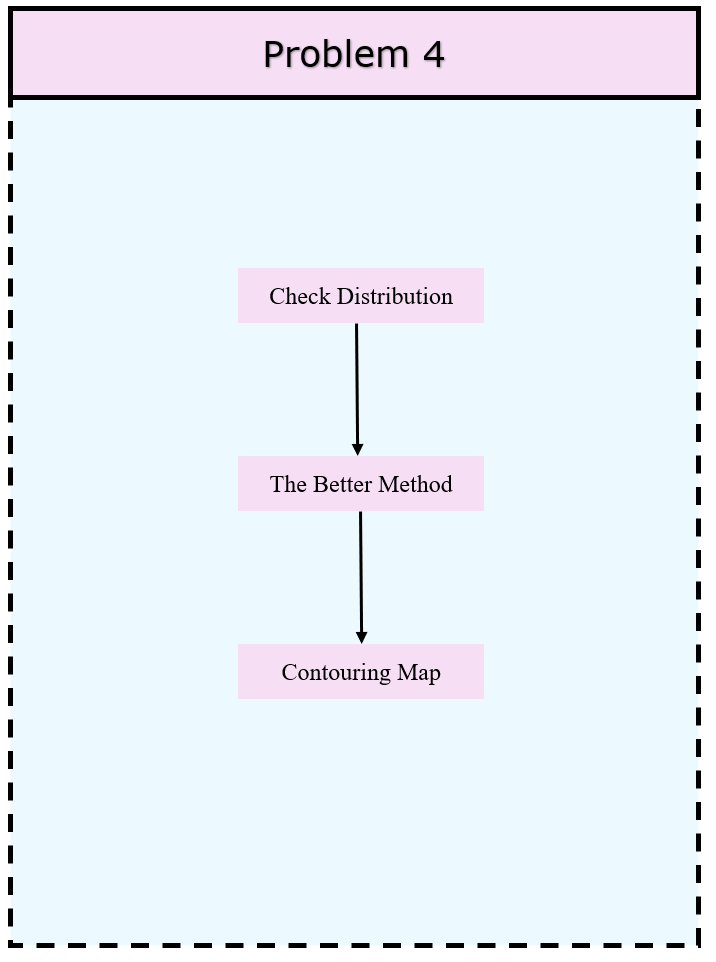
\includegraphics[width=\textwidth]{Problem 4.png}
		\caption{Problem 4 Flow Chart}
	\end{minipage}
\end{figure}


\section{General Assumptions and Notations}
\subsection{Assumptions}
\begin{itemize}
    \item Only consider spatial changes in two dimensions, ignoring latitude.
    \item  Every small region of the area should have equal possibility to be picked up as an training sample, ignoring realistic variation in difficulty, cost, efficiency and etc..
    \item Data is sufficiently accurate and unaffected by measurement interference.
    \item The correlation between the target property and the other four collaborative properties in F2 situation is the same as which in F1.
    \item The correlation between collaborative property and the main property would be remain unchanged locally and globally.
\end{itemize}

\subsection{Notations}
\begin{table}[h!t]
\centering
\begin{tabular}{cc}
\toprule[1.5pt]
Symbol & Description\\
\midrule[1pt]
$\gamma(h)$ & Variogram \\
$Z(x)$ & Spatial variable of interest \\
$h$ & Distance between two points \\
$E$ & Expectation \\
$\Delta$ & Difference between original and predicted data property\\
$p_{\text{origin}}$ & Original data property \\
$p_{\text{predicted}}$ & Predicted data property \\
$r_s$ & Spearman correlation coefficient \\
$d_i$ & Difference in ranks between the corresponding elements of two variables \\
$n$ & Number of observations \\
$Z^*(x_0)$ & Predicted value at location \(x_0\) \\
$\lambda_\alpha$ & Weights for the target variable \\
$Z(x_\alpha)$ & Observed values of the target variable \\
$\mu_{\beta1}$ & Weights for the first collaborative variable \\
$Y_1(x_\beta)$ & Observed values of the first collaborative variable \\
$\mu_{\gamma2}$ & Weights for the fourth collaborative variable \\
$Y_2(x_\gamma)$ & Observed values of the fourth collaborative variable \\
$n_{\text{closest}}$ & The number of closest points\\
$n_\text{sample\_size}$ &The number of the sample size\\
\bottomrule[1.5pt]
\end{tabular}
\end{table}


\section{Data Preprocessing and Analysis}
\subsection{Data Preprocessing}
After reviewing the provided dataset, we confirm that it contains no missing or anomalous data points. This verification upholds the integrity of the data, establishing a solid foundation for the subsequent analysis. To enhance the efficiency of data handling and analysis, we process the dataset—initially in plain text (.txt) format—using Python. This processing step successfully transforms the data into a structured format, specifically a comma-separated values (.csv) file, which facilitates organized data manipulation and analysis.

This transformation enhances the accessibility and usability of the data, allowing for more sophisticated data handling techniques to be employed in later stages. The resulting CSV file is organized into five distinct columns: 'Column Sequence', 'Row Sequence', 'X\_Coordinate', 'Y\_Coordinate' and 'Target Property'. Each column is designed to represent a specific aspect of the data, facilitating further spatial and statistical analyses. 

\subsection{Data Analysis}
After completing the data preprocessing, heatmaps for five variables from the processed dataset in Attachment 1 are generated, which visually demonstrate the spatial distribution of each variable within the study area.

\begin{figure}[h!t]
\centering
\subfigure[F1 Target]{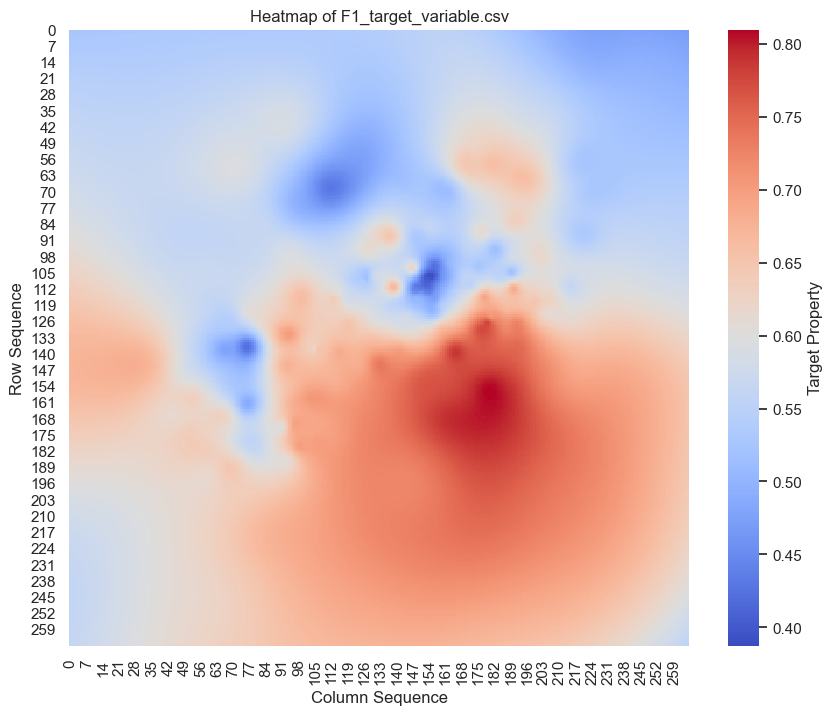
\includegraphics[width=0.485\linewidth]{Data Analysis/F1_target_分布图.png}}\hfill
\subfigure[F1 Collaborative]{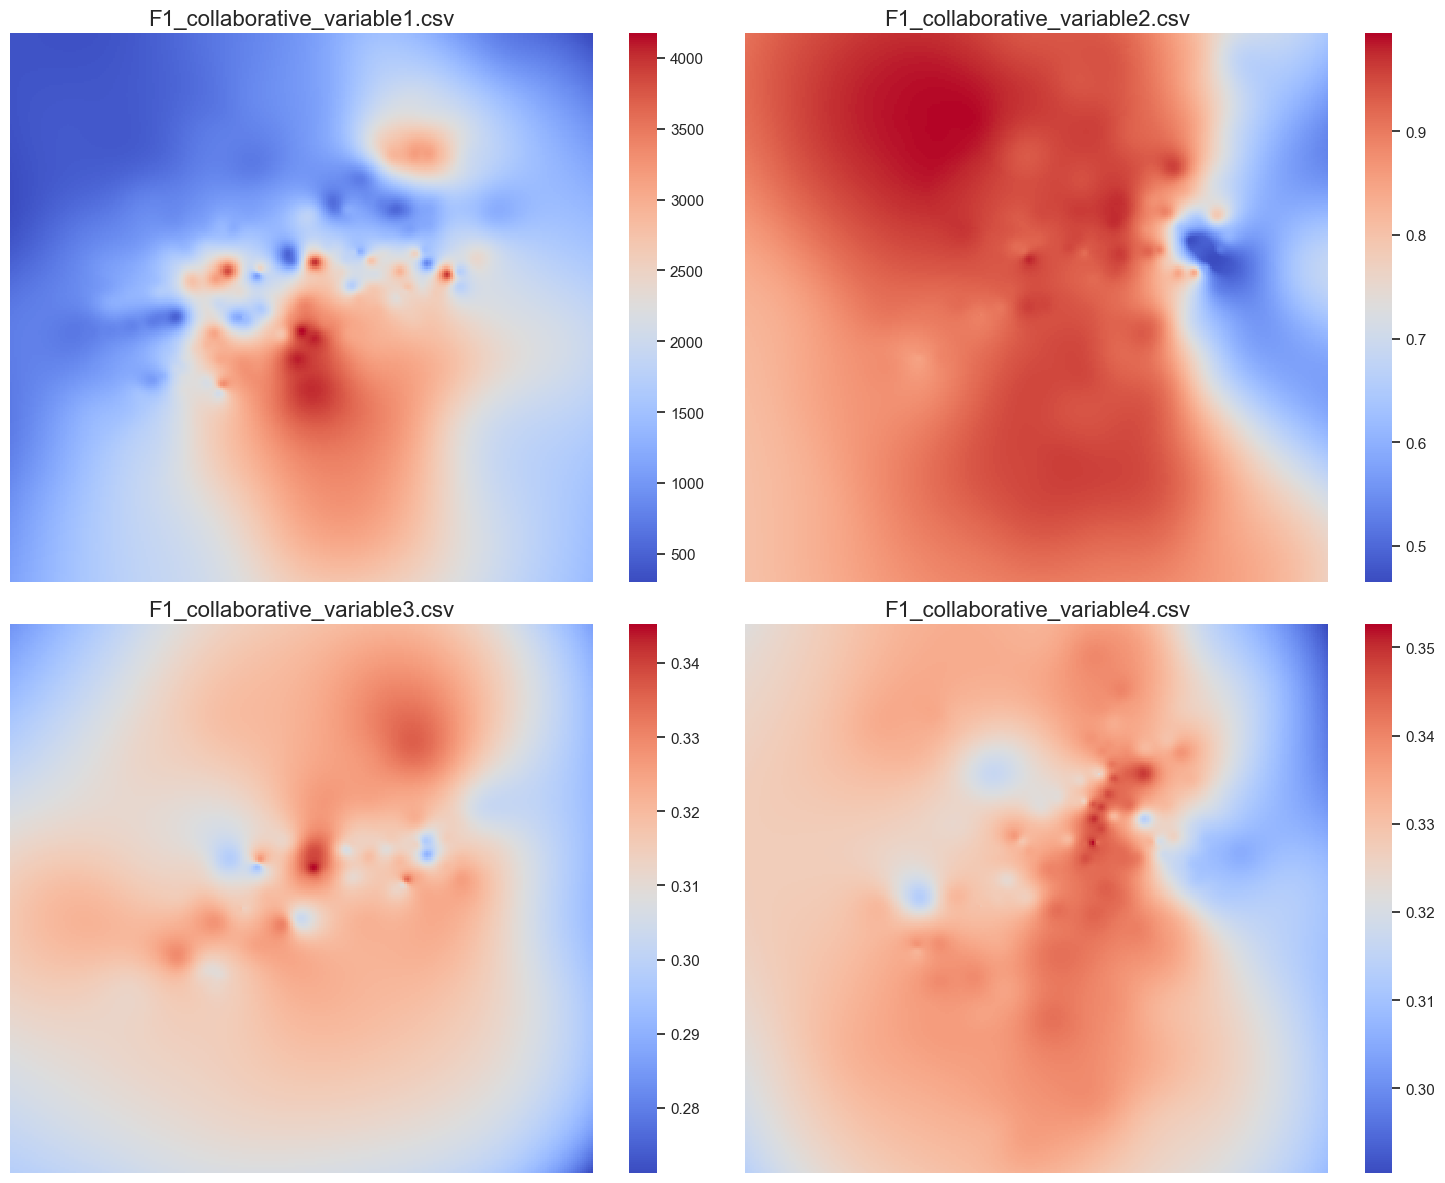
\includegraphics[width=0.485\linewidth]{Data Analysis/F1_collaborative_分布图.png}}
\caption{F1 Heat Map}
\end{figure}


Firstly, the distribution map for the Target Property illustrates the spatial trends of this attribute. The color transition from blue to red represents the shift from low to high values. This visual representation helps us identify areas with potentially higher or lower property values, which is crucial for subsequent analysis of geographical and environmental factors.

Next, the spatial distribution of four collaborative variables is analyzed. The heatmaps for these variables also use a color gradient from blue to red to indicate the magnitude of the values. Each collaborative variable's heatmap reveals distinct spatial features and distribution patterns, which are essential for understanding the relationships between variables and their potential impact on the Target Property. For instance, certain areas may show concentrations of high values for a variable, and the locations of these high-value clusters may correspond to areas of high values for the Target Property, suggesting a possible correlation between them.

Similarly, the above analysis on the datasets in Attachment 2 is conducted:

\begin{figure}[h!t]
\centering
\subfigure[F2 Target]{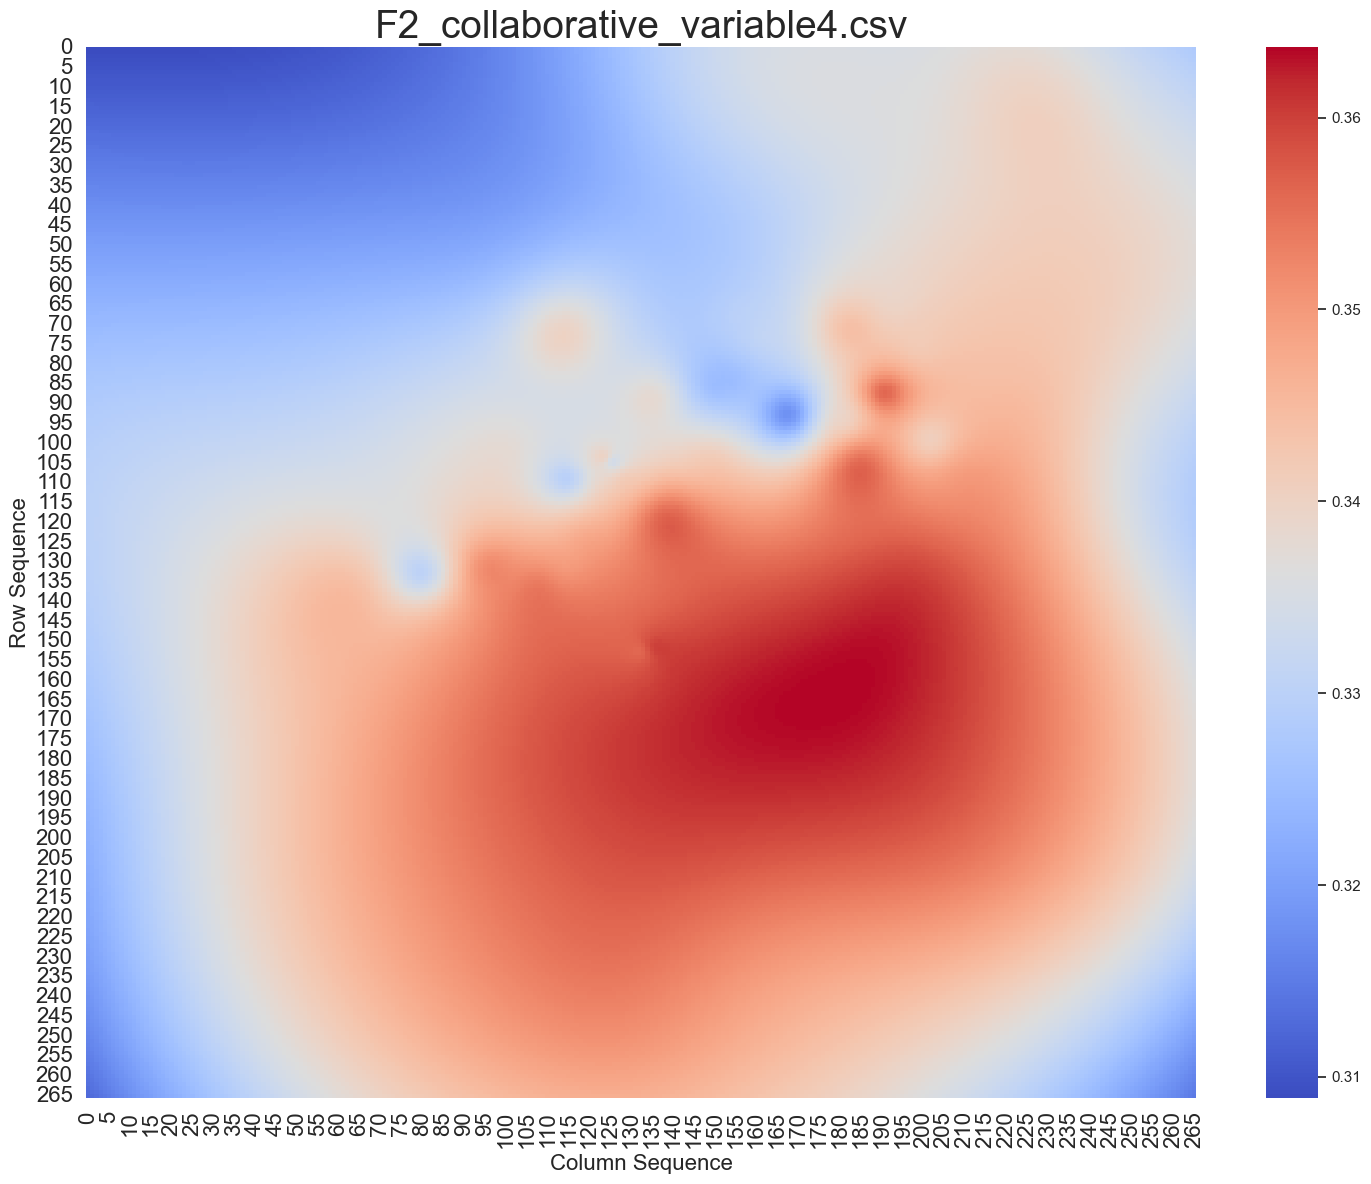
\includegraphics[width=0.485\linewidth]{Data Analysis/F2_target_分布图.png}}\hfill
\subfigure[F2 Collaborative]{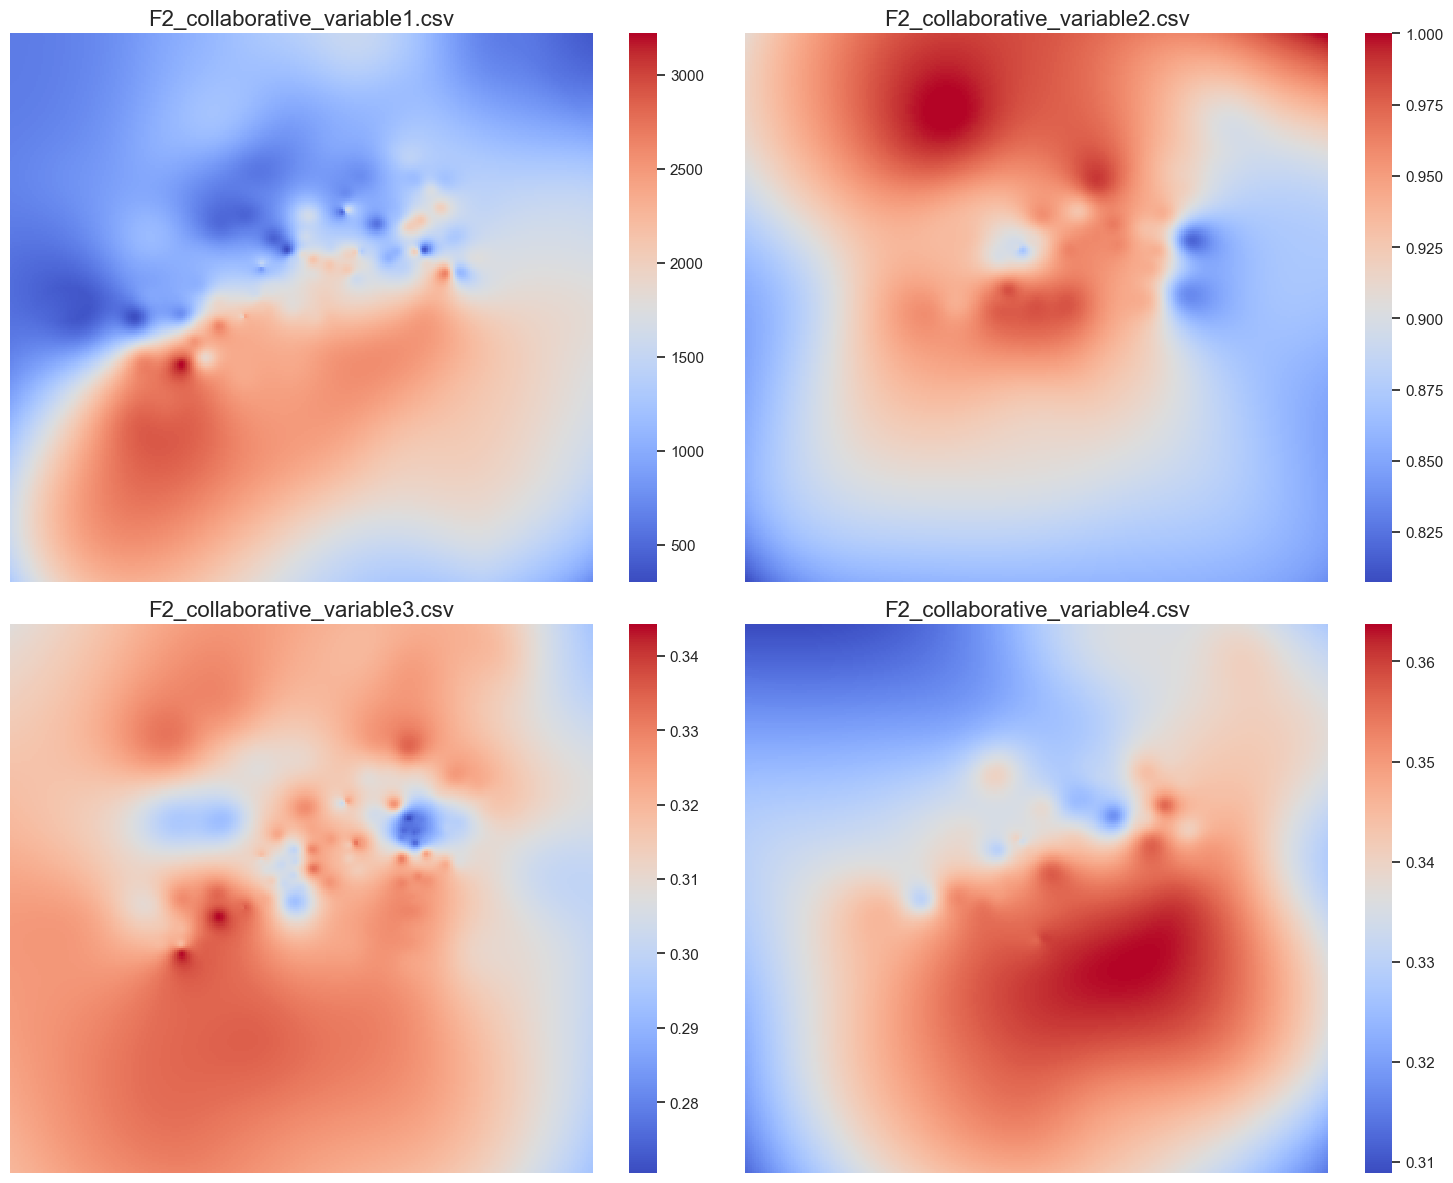
\includegraphics[width=0.485\linewidth]{Data Analysis/F2_collaborative_分布图.png}}
\caption{F2 Heat Map}
\end{figure}


\section{Problem 1}
\subsection{Spatial sequence prediction model: Kriging}
Kriging is an advanced geostatistical procedure that uses the spatial autocorrelation principle and variogram models to make predictions about geographical phenomena. It provides estimates for unknown values by not only incorporating the basic statistical properties of measured points, but also by considering the spatial correlation among them. This method is especially valued for its ability to assess the uncertainty associated with predictions, making it a robust choice for interpolating spatial data in various scientific and engineering fields.\cite{bib5}

The variogram, denoted as \(\gamma(h)\), is a fundamental concept in Kriging used to quantify the spatial autocorrelation of data points. The variogram is defined as the expected value of half the squared difference between field values at two locations separated by a vector \(h\):

\begin{equation}
\gamma(h) = \frac{1}{2} E\left[(Z(x) - Z(x + h))^2\right]
\end{equation}


We employed the Kriging algorithm using grid sampling to perform spatial analysis on a randomly selected dataset of 1000 entries from the F1 target variable database, generating a predicted contour map. Additionally, an original contour map using the complete dataset for comparison with the predicted map is created. 

\begin{figure}[h!t]
\centering
\subfigure[Predicted Property]{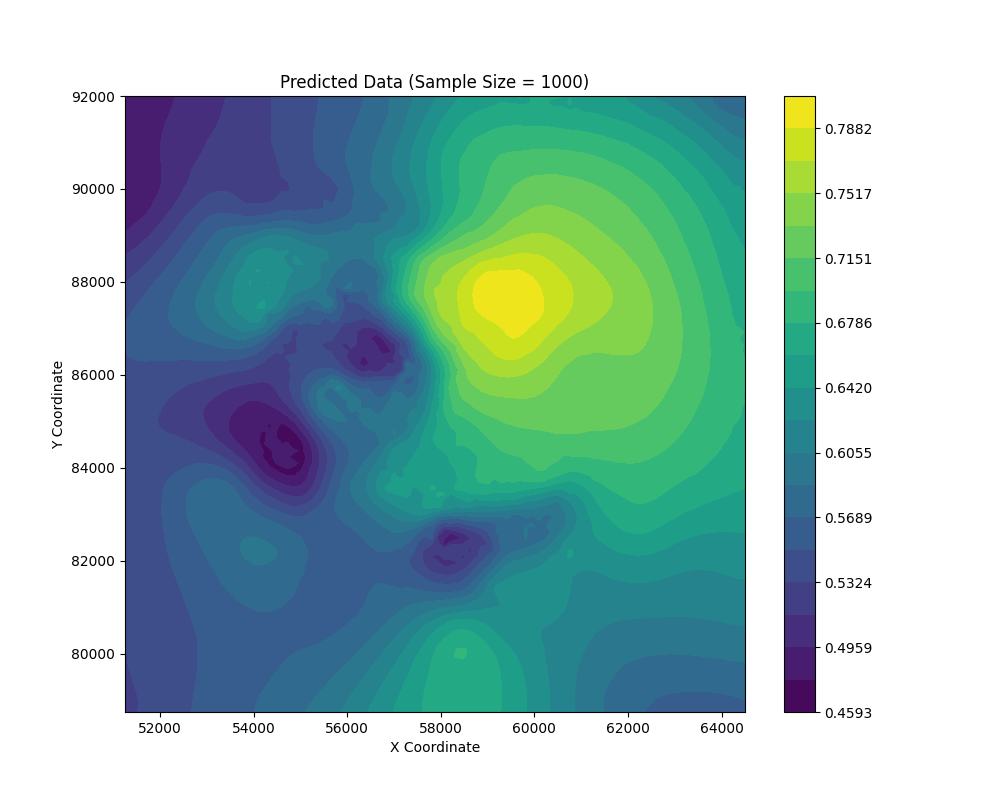
\includegraphics[width=0.485\linewidth]{Problem 1/Problem 1/Predicted_Data_Sample_Size_1000.png}}\hfill
\subfigure[Origin Property]{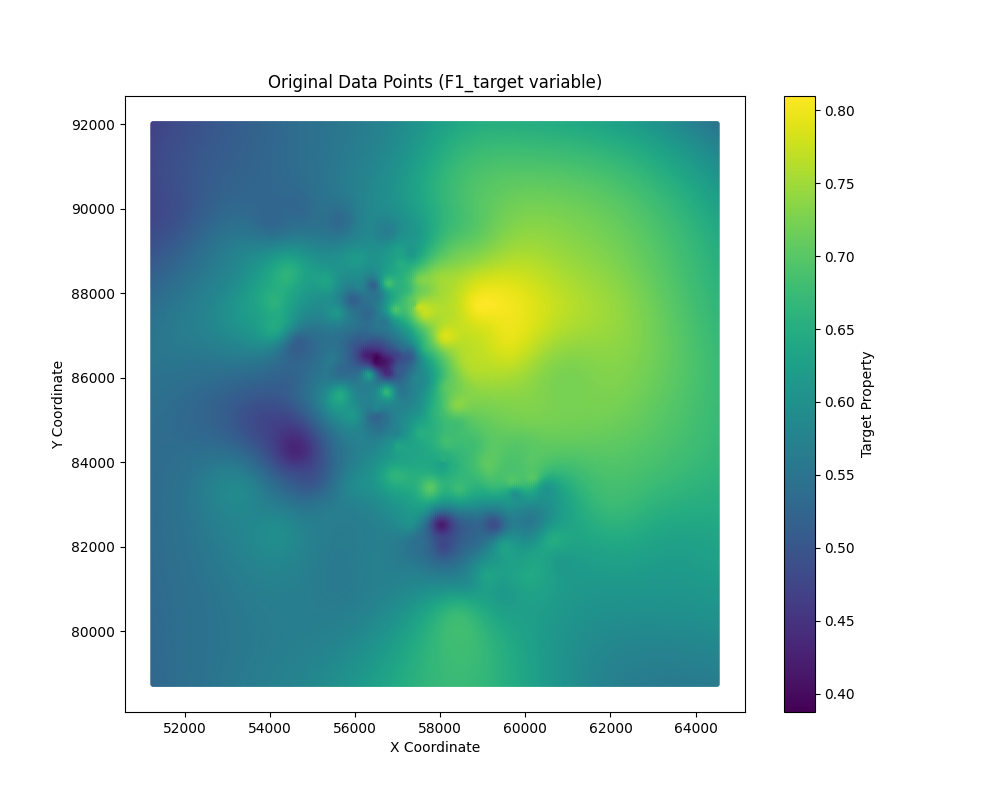
\includegraphics[width=0.485\linewidth]{Problem 1/Problem 1/Original_Data_Points.png}}
\caption{Sample size 1000 results}
\end{figure}

To thoroughly evaluate the predictive effectiveness of the Kriging algorithm, we generated a difference map by calculating the discrepancies between the original data and the predicted data. The formula for calculating the difference is defined as:

\begin{equation}
\Delta = p_{\text{origin}} - p_{\text{predicted}}
\end{equation}

Using the steps outlined above, we generate the following graphs, which visually assess the accuracy of the predictions across different spatial distributions. In these difference maps, red areas indicate regions where the predicted values exceed the actual values, while blue areas represent regions where the predicted values fall short. These maps provide essential visual feedback, helping us identify variations in the model’s performance across different areas, and enabling further adjustments and optimizations.

\begin{figure}[h!t]
	\centering
	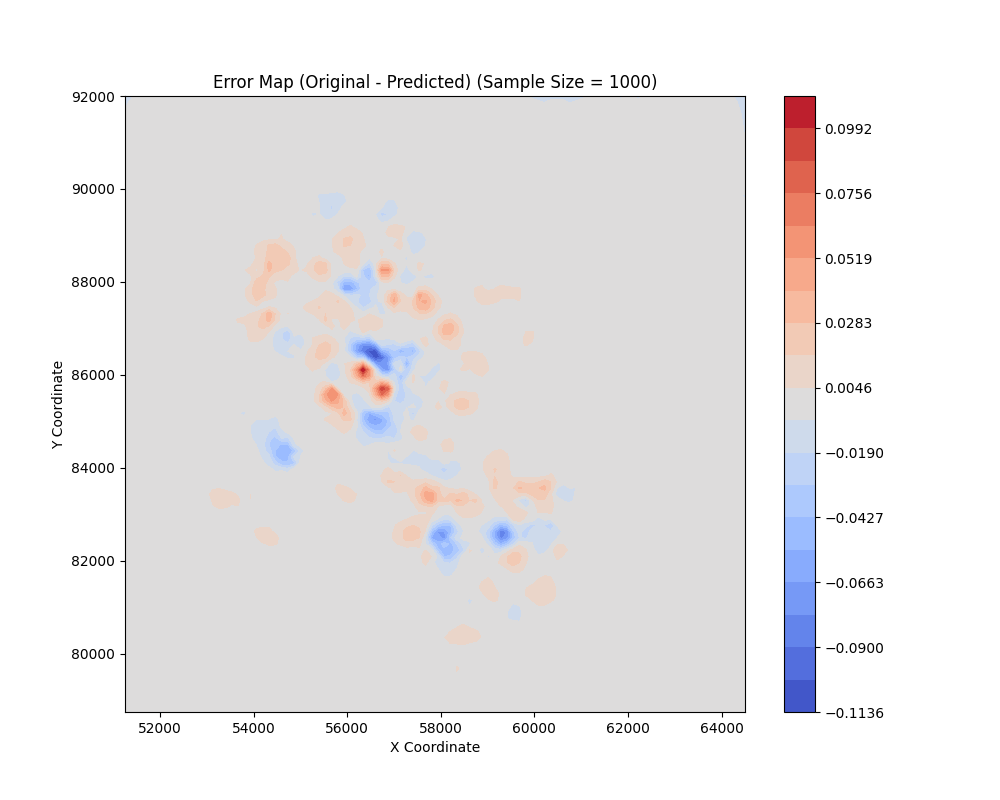
\includegraphics[width=0.9\textwidth]{Problem 1/Problem 1/Error_Map_Sample_Size_1000.png}
	\caption{Error Map 1000}
\end{figure}

We observe that using reference points that are too distant in Kriging interpolation can lead to significant errors. Therefore, careful selection of reference points is crucial. To address this, we employ the Kernel Density Estimation (KDE) algorithm to locate nearby points, which enhances computational efficiency and reduces memory usage. Additionally, we develop a custom function to determine the optimal number of nearby points to consider in the Kriging algorithm. These enhancements are designed to optimize the model's performance and adaptability in handling spatial data.

\subsection{Effect of Sample Size Variations on Results}

To thoroughly investigate the impact of sample size on the accuracy of spatial estimations, we systematically vary the number of data points sampled. We perform random samplings of 50, 200, 500, 8000, 25000, and 50000 points to explore how increasing the sample size influences the estimation error. For each sample size, we follow the methodology outlined in Section 4.1 of the study to generate the corresponding Origin Property and Predicted Property maps. Error maps are then produced to visually represent the discrepancies between the predicted values and the actual measurements. This comprehensive approach enables us to assess the performance of the predictive model under varying conditions of data availability, providing valuable insights into the trade-offs between sample size and prediction accuracy.

\begin{figure}[h!t]
\centering
\subfigure[Predicted 50]{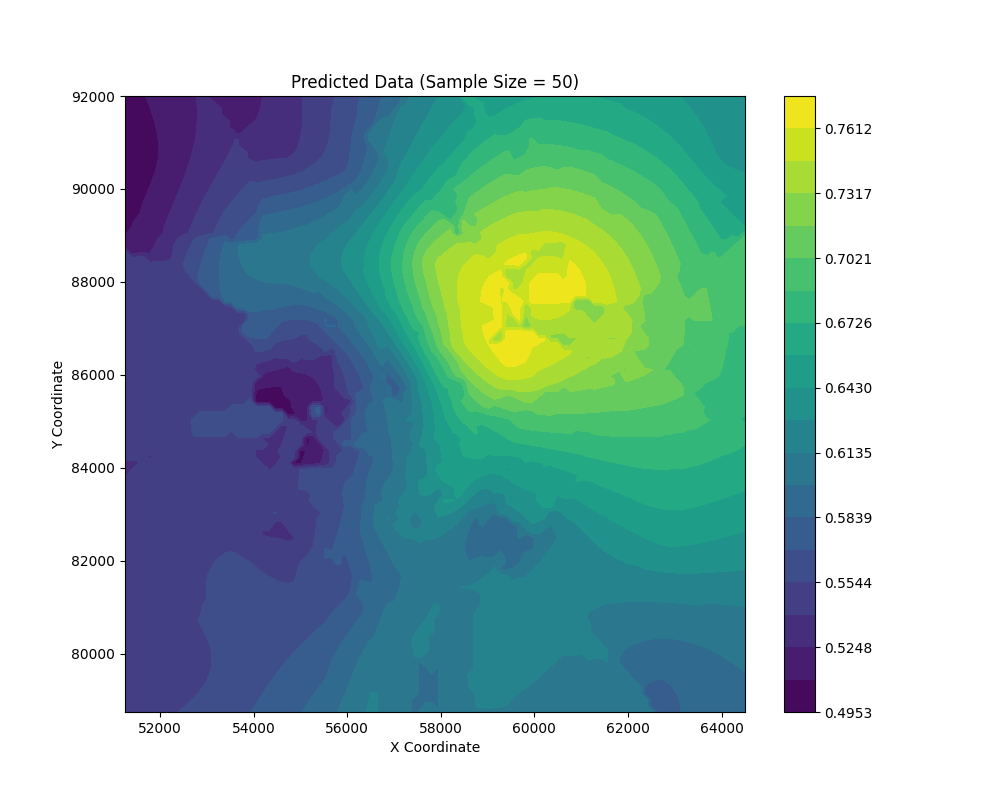
\includegraphics[width=0.23\linewidth]{Problem 1/Problem 1/Predicted_Data_Sample_Size_50.png}}
\subfigure[Error Map 50]{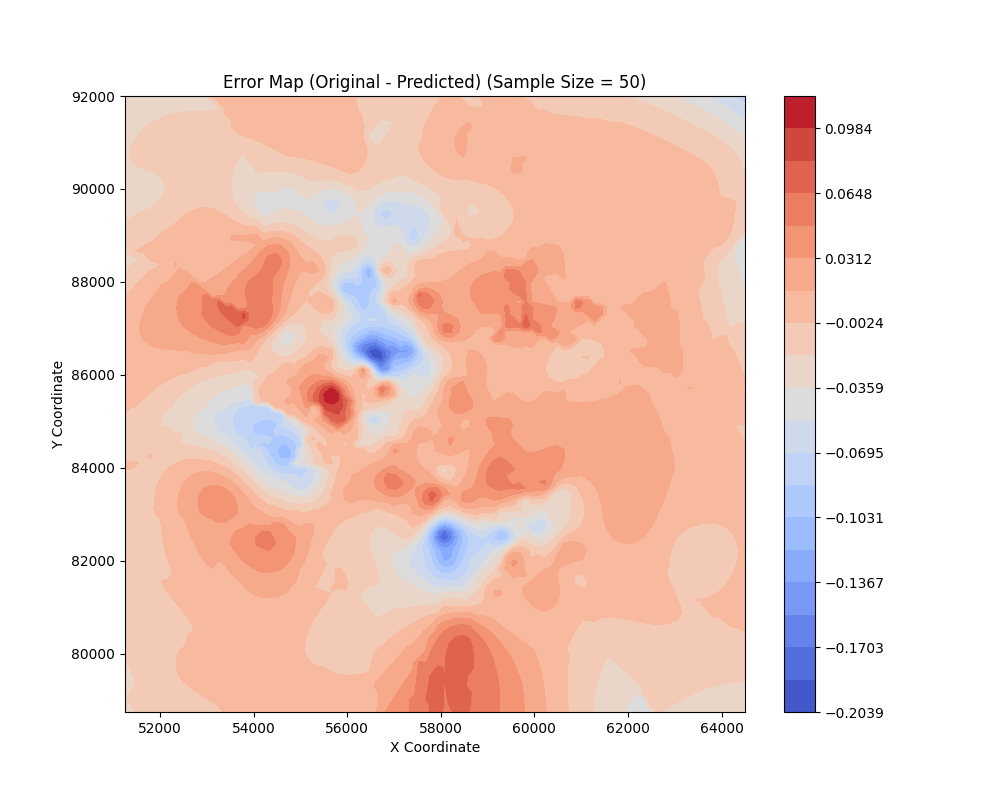
\includegraphics[width=0.23\linewidth]{Problem 1/Problem 1/Error_Map_Sample_Size_50.png}}
\subfigure[Predicted  200]{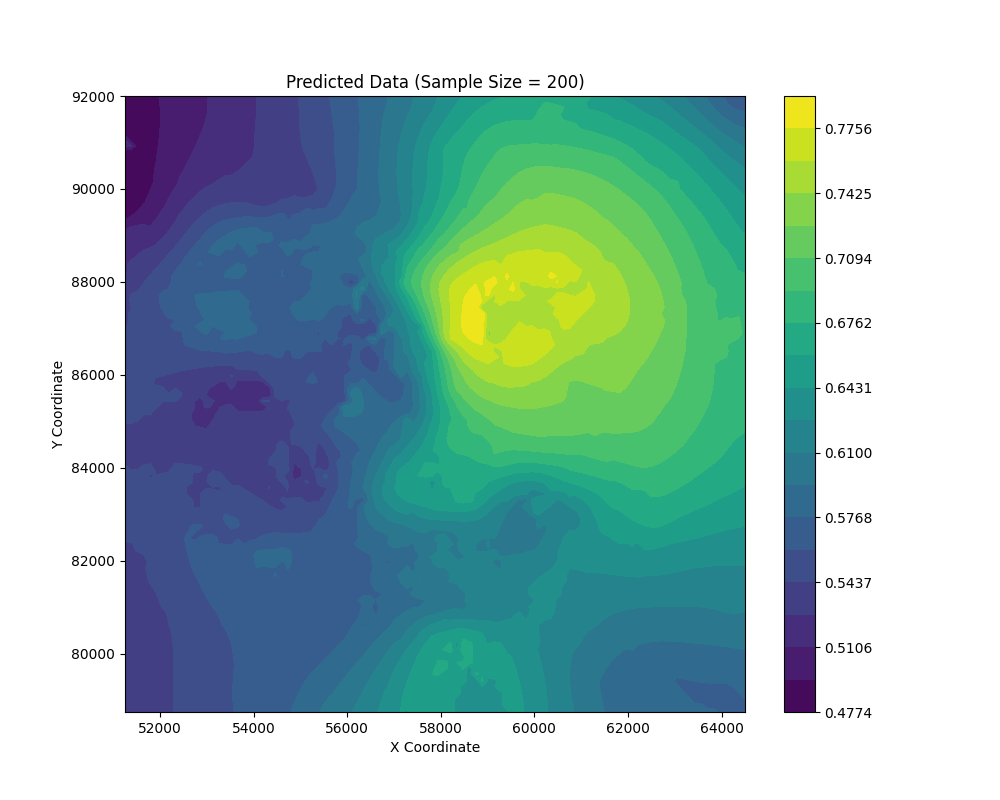
\includegraphics[width=0.23\linewidth]{Problem 1/Problem 1/Predicted_Data_Sample_Size_200.png}}
\subfigure[Error Map 200]{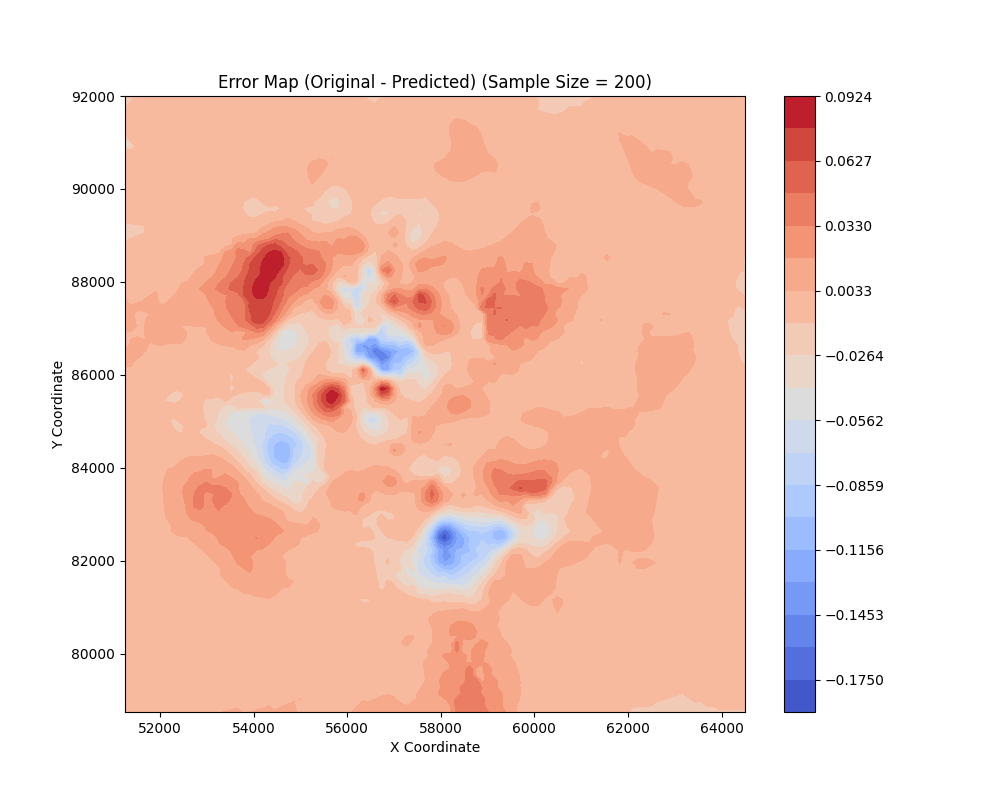
\includegraphics[width=0.23\linewidth]{Problem 1/Problem 1/Error_Map_Sample_Size_200.png}}

\subfigure[Predicted  500]{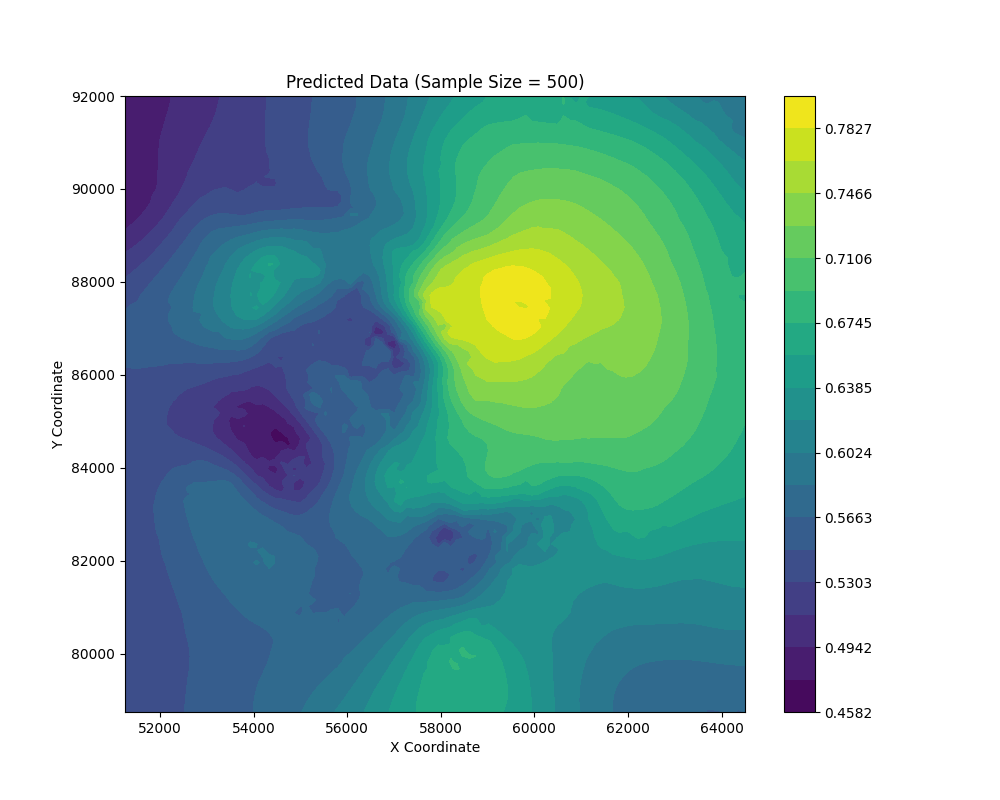
\includegraphics[width=0.23\linewidth]{Problem 1/Problem 1/Predicted_Data_Sample_Size_500.png}}
\subfigure[Error Map 500]{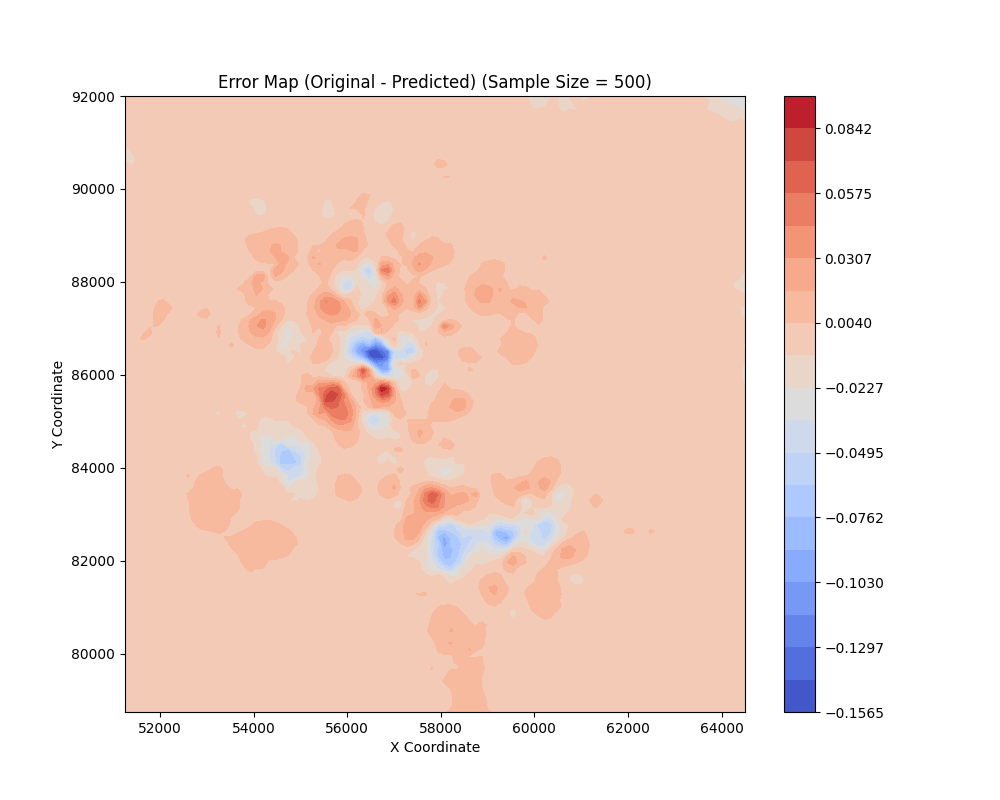
\includegraphics[width=0.23\linewidth]{Problem 1/Problem 1/Error_Map_Sample_Size_500.png}}
\subfigure[Predicted  8000]{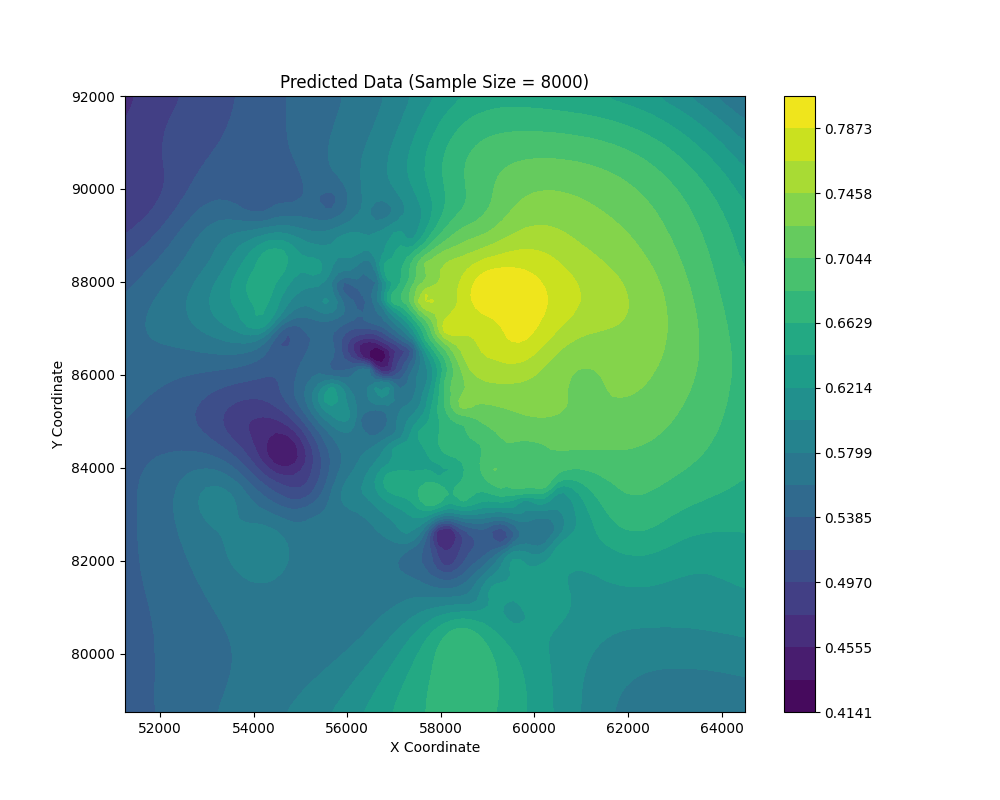
\includegraphics[width=0.23\linewidth]{Problem 1/Problem 1/Predicted_Data_Sample_Size_8000.png}}
\subfigure[Error Map 8000]{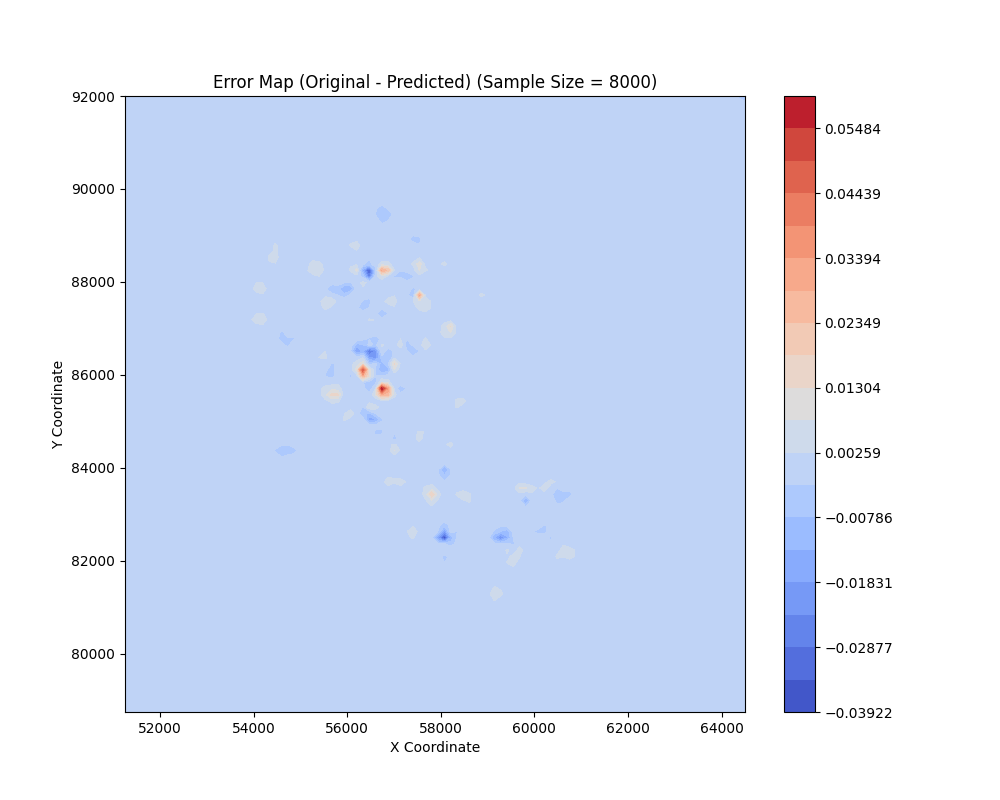
\includegraphics[width=0.23\linewidth]{Problem 1/Problem 1/Error_Map_Sample_Size_8000.png}}

\subfigure[Predicted  25000]{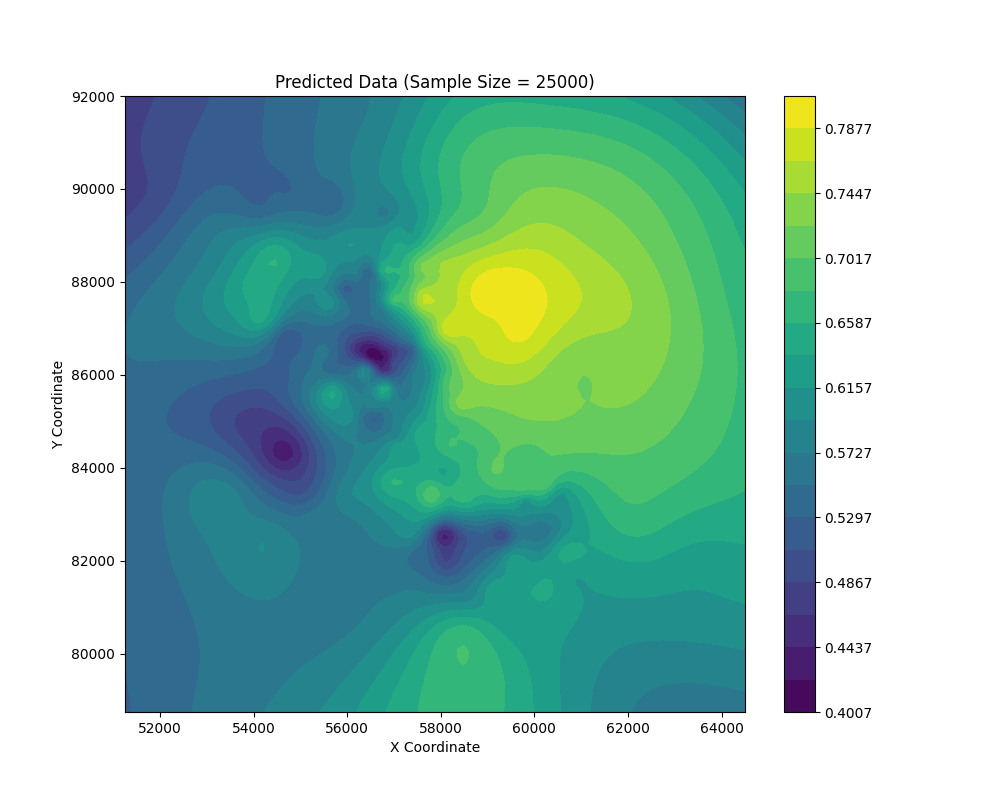
\includegraphics[width=0.23\linewidth]{Problem 1/Problem 1/Predicted_Data_Sample_Size_25000.png}}
\subfigure[Error Map 25000]{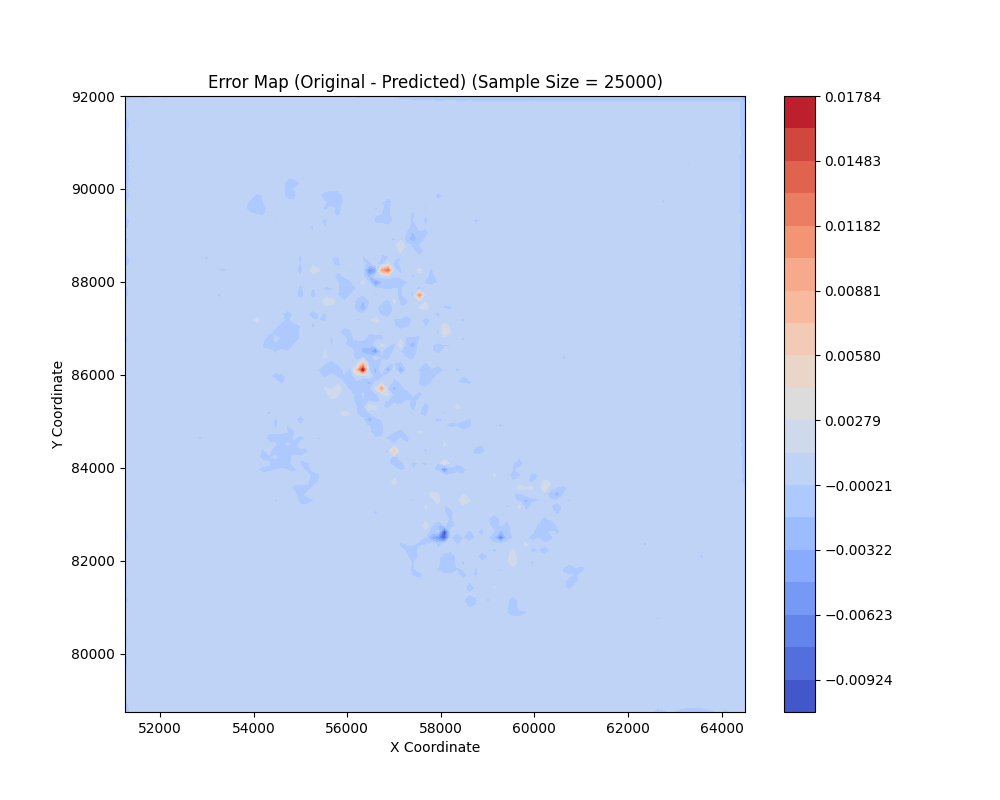
\includegraphics[width=0.23\linewidth]{Problem 1/Problem 1/Error_Map_Sample_Size_25000.png}}
\subfigure[Predicted  50000]{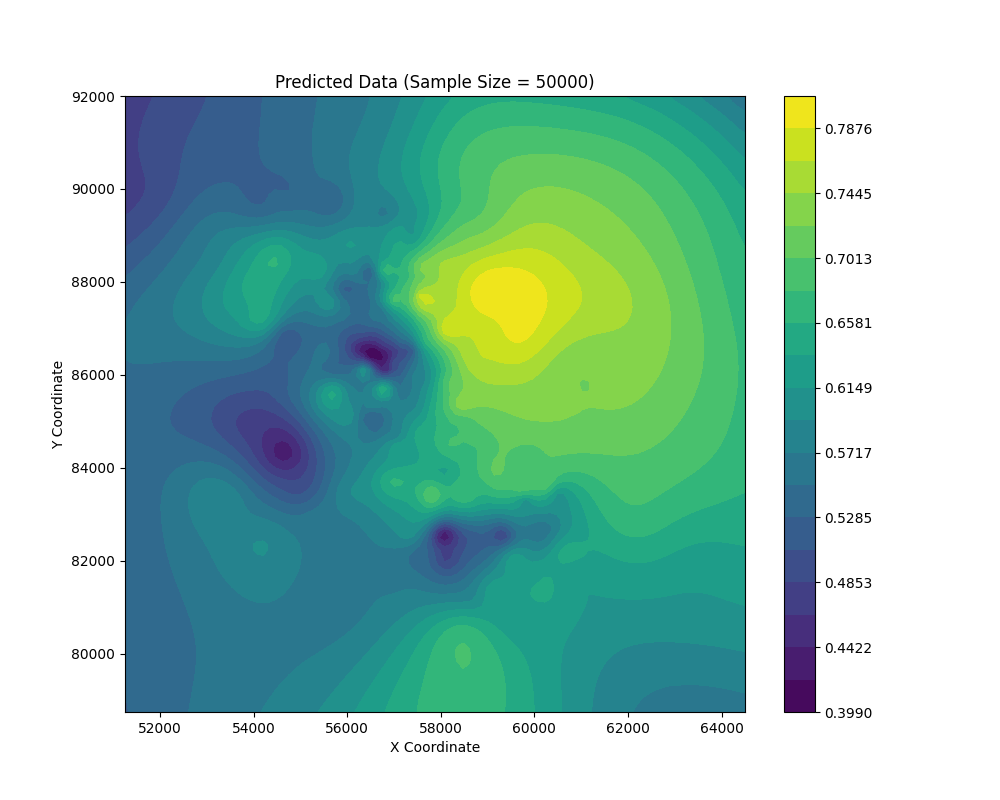
\includegraphics[width=0.23\linewidth]{Problem 1/Problem 1/Predicted_Data_Sample_Size_50000.png}}
\subfigure[Error Map 50000]{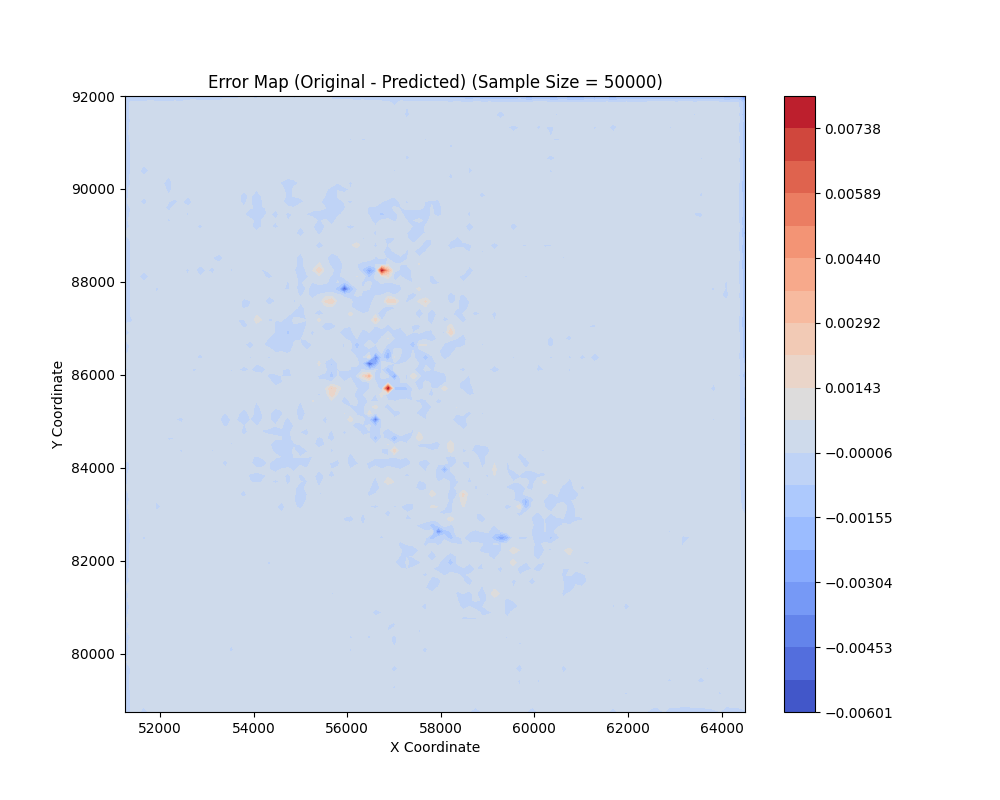
\includegraphics[width=0.23\linewidth]{Problem 1/Problem 1/Error_Map_Sample_Size_50000.png}}

\caption{Results for Predicted Property and Error Maps at Different Sample Sizes}
\label{fig:four_per_row_23}
\end{figure}

\subsection{Correlation Between Sample Size and Estimation Accuracy}

In the spatial analysis using Kriging, we systematically vary the sample size and analyze the resulting error maps to examine the relationship between sample size and estimation accuracy. These error maps visually represent discrepancies between the predicted and actual values: red areas indicate where the model overestimates, while blue areas show where it underestimates the values.

The analysis starts with a sample size of 1000 data points and progressively includes 50, 200, 500, 8000, 25000, and 50000 data points. The results, as shown in the table, reveal a clear trend: as the sample size increases, both the overall error and the variability of error across the map generally decrease. Notably, maps based on smaller sample sizes exhibit larger fluctuations and more pronounced areas of red and blue, indicating significant overestimations and underestimations.

\begin{table}[h!]
\centering
\caption{Kriging Performance Metrics}
\label{tab:sample_size_metrics}
\begin{tabular}{|c|c|c|c|c|}
\hline
\textbf{Sample Size} & \textbf{Percentage of Total} & \textbf{MSE} & \textbf{RMSE} & \textbf{MAE} \\ \hline
50     & 0.07\%  & 0.000822 & 0.028667 & 0.019045 \\ \hline
200    & 0.28\%  & 0.000456 & 0.021356 & 0.010552 \\ \hline
500    & 0.71\%  & 0.000013 & 0.011404 & 0.004465 \\ \hline
1000   & 1.41\%  & 0.000063 & 0.007949 & 0.002713 \\ \hline
8000   & 11.31\% & 0.000003 & 0.001742 & 0.000402 \\ \hline
25000  & 35.33\% & 0 & 0.00496  & 0.000139 \\ \hline
50000  & 70.67\% & 0 & 0.00307  & 0.00009  \\ \hline
\end{tabular}
\end{table}

The specific data from the table illustrate that as the sample size increases from 50 to 50000, there is a noticeable downward trend in MSE (Mean Squared Error), RMSE (Root Mean Squared Error), and MAE (Mean Absolute Error). For example, when the sample size is 50, the MSE is 0.000822, which decreases to 0.00307 when the sample size reaches 50000. This trend demonstrates that as more data points are available, the Kriging model can more accurately capture and model spatial dependencies, thereby improving the accuracy of predictions.

As the sample size increases, particularly when it reaches 25,000 and above, accounting for over 35.33\% of the entire dataset, the error maps exhibit much subtler variations in color, indicating that the model’s predictions are becoming more consistent and closer to the actual values. This improvement in prediction accuracy with increasing sample size underscores the importance of using sufficient data samples in spatial prediction models to minimize prediction errors and achieve higher reliability in the results. It also highlights the utility of Kriging in handling large spatial datasets, optimizing its parameters, and refining predictions as more data becomes accessible.

\section{Problem 2}
In the process of handling this dataset, we initially apply normalization and standardization techniques to ensure a uniform distribution of data points. This preprocessing step is crucial as it enhances the reliability and effectiveness of the subsequent statistical analyses. After that, we conduct QQ-plot normality tests to help determine if the Pearson correlation coefficient, a measure of linear correlation between two variables, can appropriately describe the relationship, or if other non-parametric methods should be considered due to deviations from a normal distribution. This step is essential to validate the use of statistical methods that assume normality in the data for accurate results.
\begin{figure}[h!t]
	\centering
	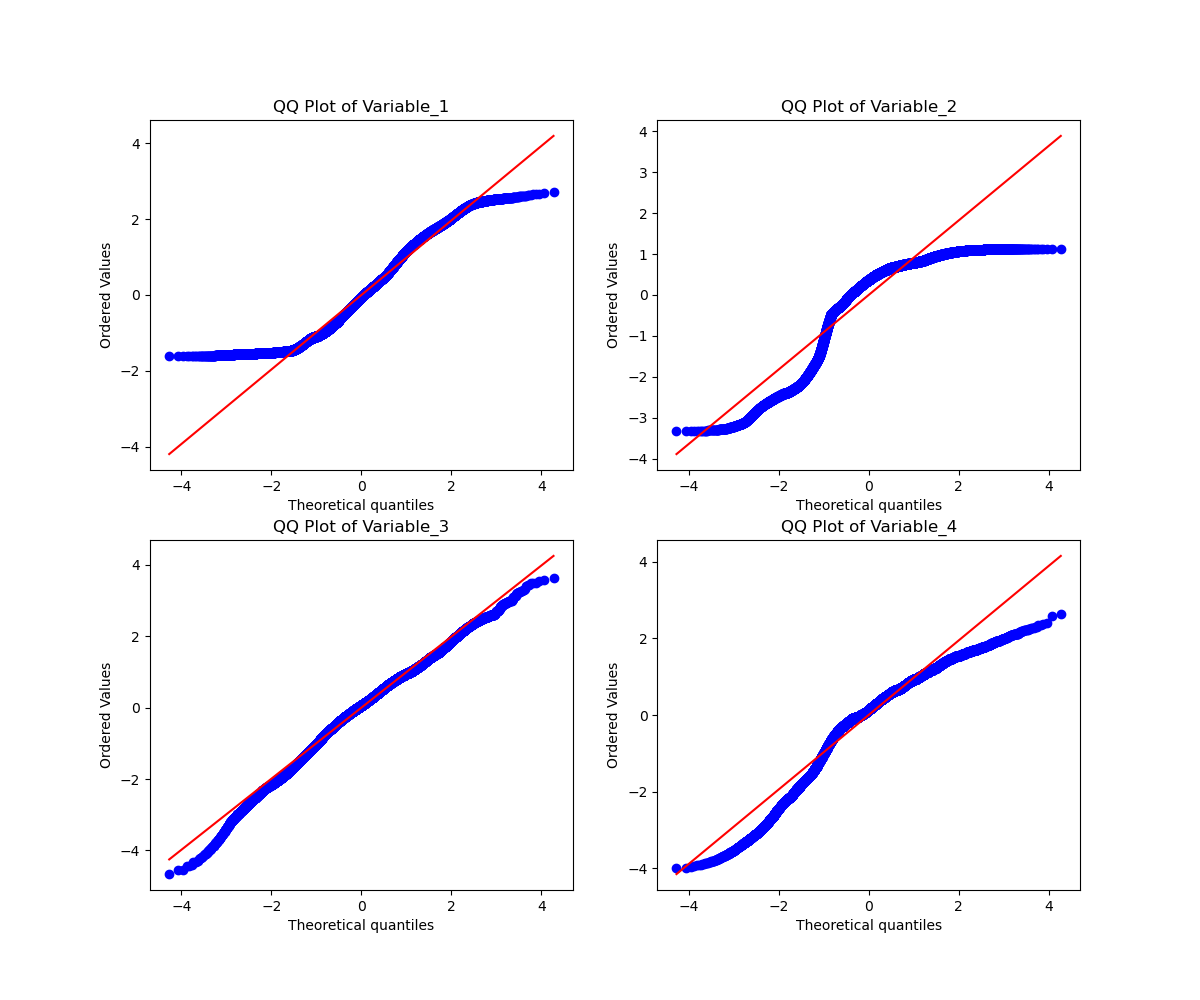
\includegraphics[width=0.6\textwidth]{Problem 2/Problem 2/QQ Plot.png}
	\caption{QQ-plot}
\end{figure}

The results of the QQ-plot normality test indicate that only variables 3 and 4 exhibit some degree of normality, whereas variables 1 and 2 do not show significant characteristics of normal distributions. Given that not all variables conform to a normal distribution, we opt to use Spearman's rank correlation coefficient for assessing the relationships between variables. Spearman's coefficient is preferable for non-linear or non-normally distributed data. The Spearman's coefficient calculation function is shown below:

\begin{equation}
    r_s = 1 - \frac{6 \sum d_i^2}{n(n^2 - 1)}
\end{equation}

\vspace{1.5em}
\noindent The results of the Spearman correlation analysis are as follows:

\begin{table}[h!]
\caption{Spearman correlation coefficients between collaborative variables and the target variable.} % 表格标题在上
\centering
\begin{tabular}{|c|c|c|}
\hline
Variable & Spearman Coefficient & Correlation Type \\ \hline
1 & 0.749863404549425 & Strong positive \\ \hline
2 & -0.095762502927994 & Slight negative \\ \hline
3 & 0.1257393627897889 & Slight positive \\ \hline
4 & 0.317949911485028 & Moderate positive \\ \hline
\end{tabular}
\label{tab:spearman_coefficients}
\end{table}

To further explore the distribution relationships between each variable and the target variable, we plot four different two-dimensional Kernel Density Estimation (2D-KDE) graphs using subplots. These 2D-KDE plots effectively illustrate the joint distribution characteristics between each variable and the target variable, helping us visually understand the interactions between variables and their potential impact patterns. By comparing these KDE plots, clearer distribution trends between each variable and the target variable emerge, providing valuable references for further analysis and model development. Except for collaborative variable 1, which demonstrates linear correlation, the other variables do not exhibit such a relationship.

\begin{figure}[h!t]
	\centering
	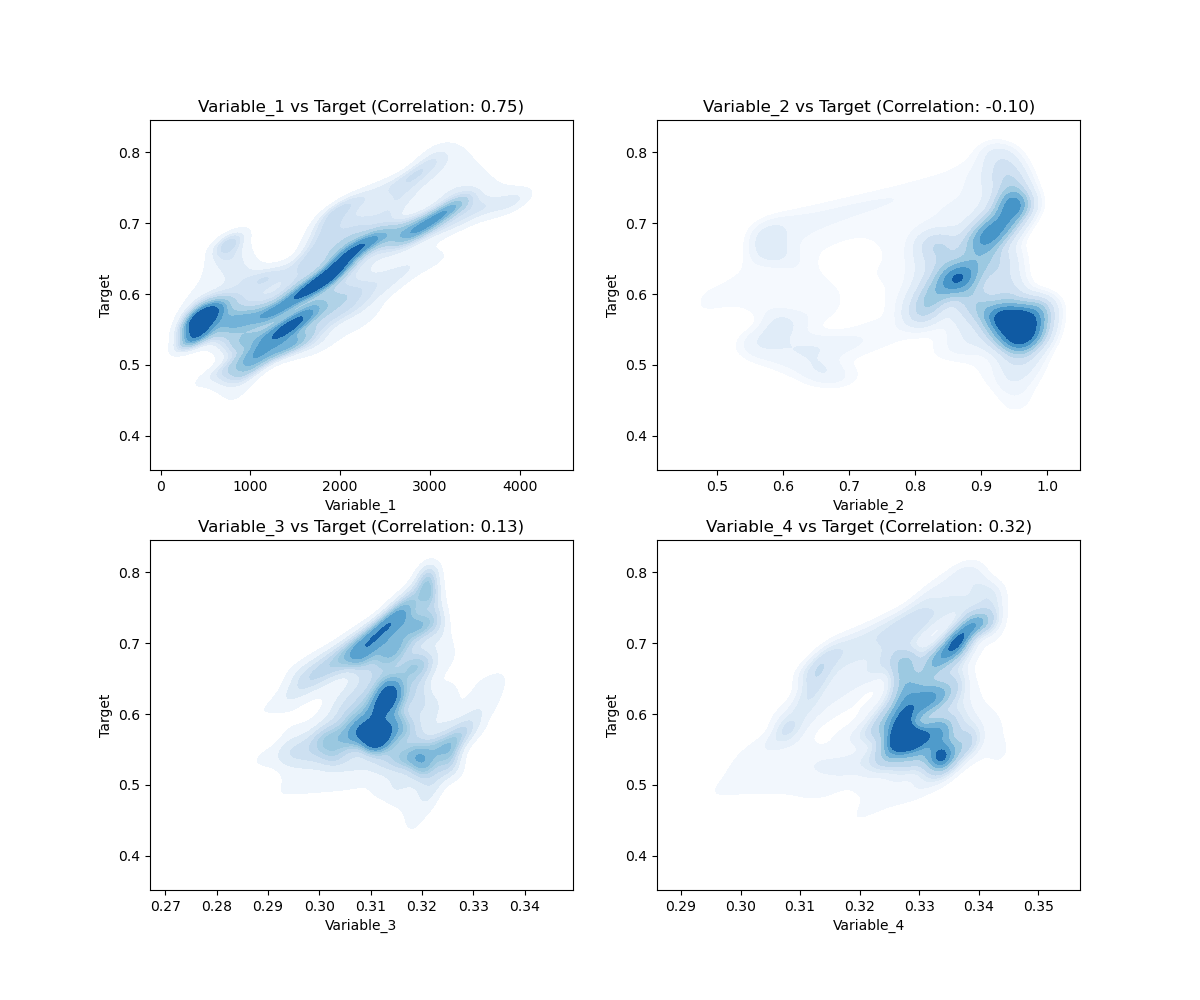
\includegraphics[width=0.8\textwidth]{Problem 2/Problem 2/2D Kernel Density Estimation Plot.png}
	\caption{2D-KDE}
\end{figure}

Based on the comprehensive analysis, Variables 1 and 4 are chosen for further investigation. These variables demonstrate strong correlations and interesting distribution characteristics, which are expected to play a crucial role in model development, especially in predicting the target variable. This selection will help optimize the analytical model, ensuring that it is sensitive and accurate in responding to key variables, thereby enhancing the accuracy and reliability of the model predictions.

\section{Problem 3}
\subsection{Co-Kriging}
In Co-Kriging, the determination of weights is accomplished through an automated calculation aimed at minimizing the variance of the prediction error while ensuring that the estimate is unbiased. This calculation relies on the spatial autocorrelation between the primary variable and one or more secondary variables, as well as their respective relationships with the prediction location.

The calculation of the weights involves solving a system of linear equations, where the coefficient matrix consists of the semivariances (or covariances) among the variables. Specifically, this matrix includes the variogram of the primary variable, the variograms of each secondary variable, and the cross-variograms between the primary and each secondary variable. The system also includes a term known as a Lagrange multiplier, which ensures the unbiasedness of the estimate.

The weights derived from solving this system are then directly applied in the Co-Kriging formula to predict the target property values at unknown locations. In this way, Co-Kriging leverages information from multiple correlated variables, providing more precise and reliable spatial data predictions compared to simple Kriging.

Basic Formula of Co-Kriging is as follows:

\begin{equation}
Z^*(x_0) = \sum_{\alpha=1}^n \lambda_\alpha Z(x_\alpha) + \sum_{\beta=1}^m \mu_{\beta} Y(x_{\beta})   
\end{equation}

We have now selected two collaborative variables, so the formula will become:

\begin{equation}
Z^*(x_0) = \sum_{\alpha=1}^n \lambda_\alpha Z(x_\alpha) + \sum_{\beta=1}^m \mu_{\beta1} Y_1(x_{\beta}) + \sum_{\gamma=1}^p \mu_{\gamma2} Y_2(x_{\gamma}) 
\end{equation}

\subsubsection{Innovative Approach - cKDTree}

In this work, an innovative approach is introduced to enhance the computational efficiency of Co-Kriging by incorporating a nearest-neighbor search algorithm (cKDTree). Rather than considering all data points for each interpolation, we use the cKDTree method to quickly identify the nearest neighbors for each grid point. This significantly reduces the number of points considered in the Kriging interpolation, enabling faster calculations while maintaining the accuracy of the predictions. The identified nearest neighbors are then used to derive the appropriate weights, optimizing the Kriging process for large datasets.

The number of closest points ($n_{\text{closest}}$) selected for each interpolation is determined based on the sample size ($n_{\text{sample\_size}}$) using the following formula:

\begin{equation}
n_{\text{closest}} = \left(\frac{1}{n_\text{sample\_size}+2000} \times 10000 + 10 \right)
\end{equation}

This formula is designed to dynamically adjust the number of neighbors based on the size of the dataset. As the sample size increases, the number of nearest neighbors decreases, ensuring a balance between efficiency and quality. This approach allows Kriging computing faster while considering a sufficient number of data points to capture the spatial dependencies in the data.

\subsubsection{Co-Kriging Results}

Using the approach from Problem 1, the following results are obtained:

\begin{figure}[h!t]
\centering
\subfigure[Predicted Property 1000]{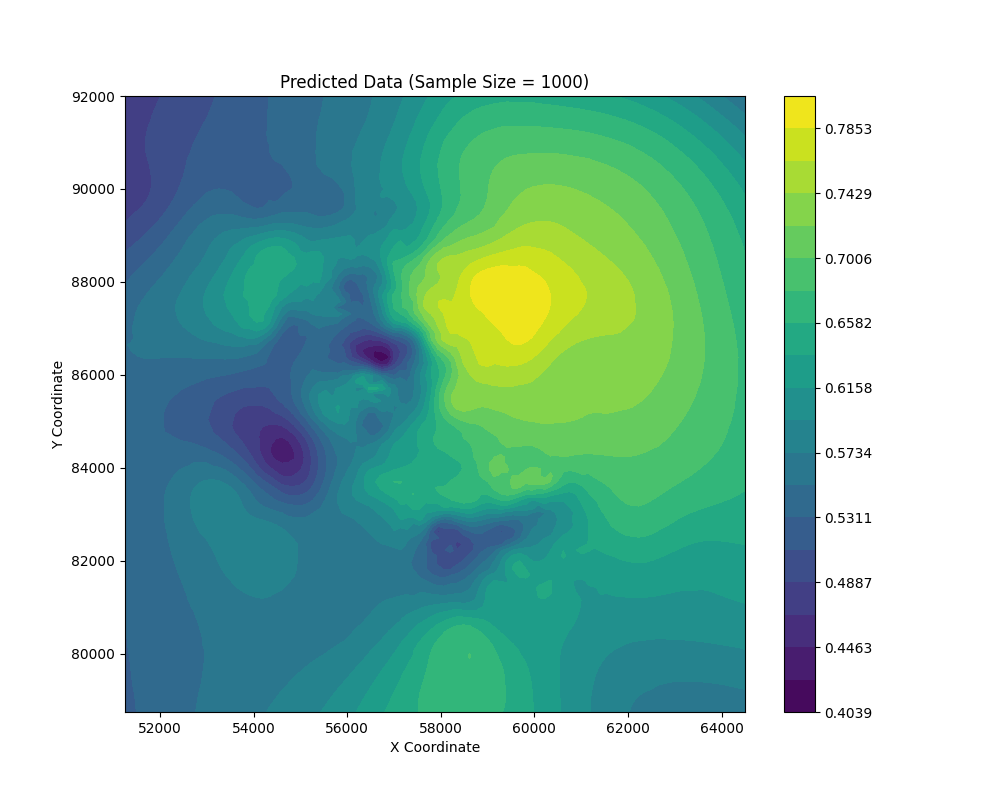
\includegraphics[width=0.3\linewidth]{Problem 3/Problem 3/Co-Kriging/Predicted_Data_Sample_Size_1000.png}}
\hfill
\subfigure[Origin Property]{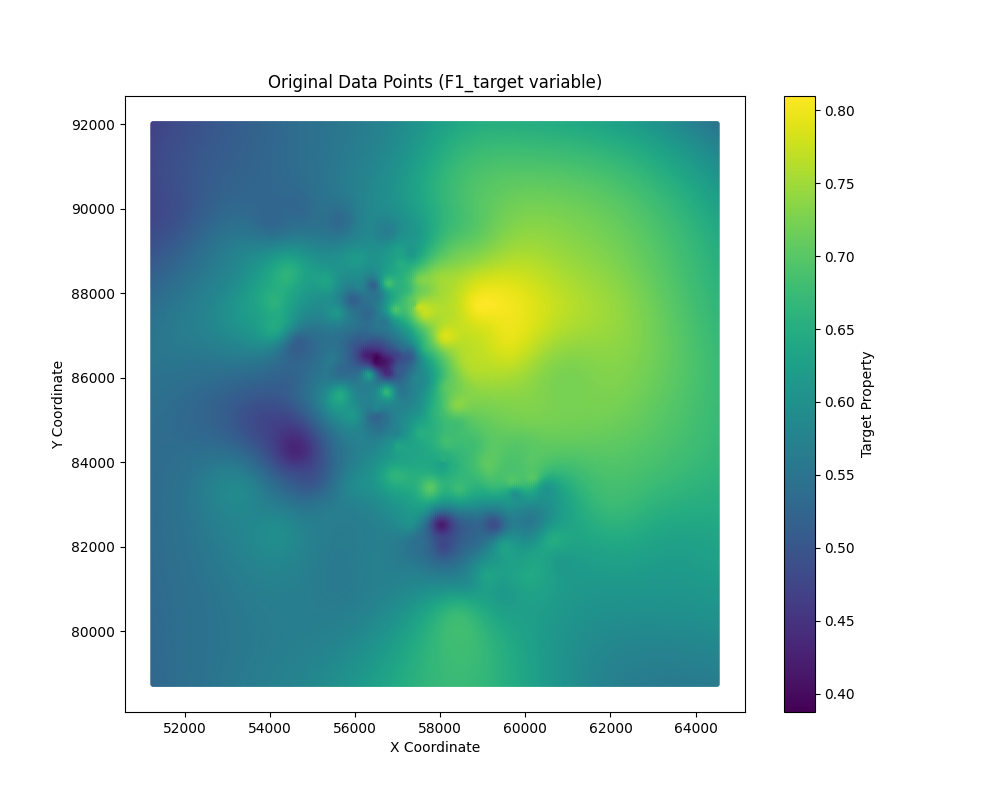
\includegraphics[width=0.3\linewidth]{Problem 1/Problem 1/Original_Data_Points.png}}
\hfill
\subfigure[Error Map 1000]{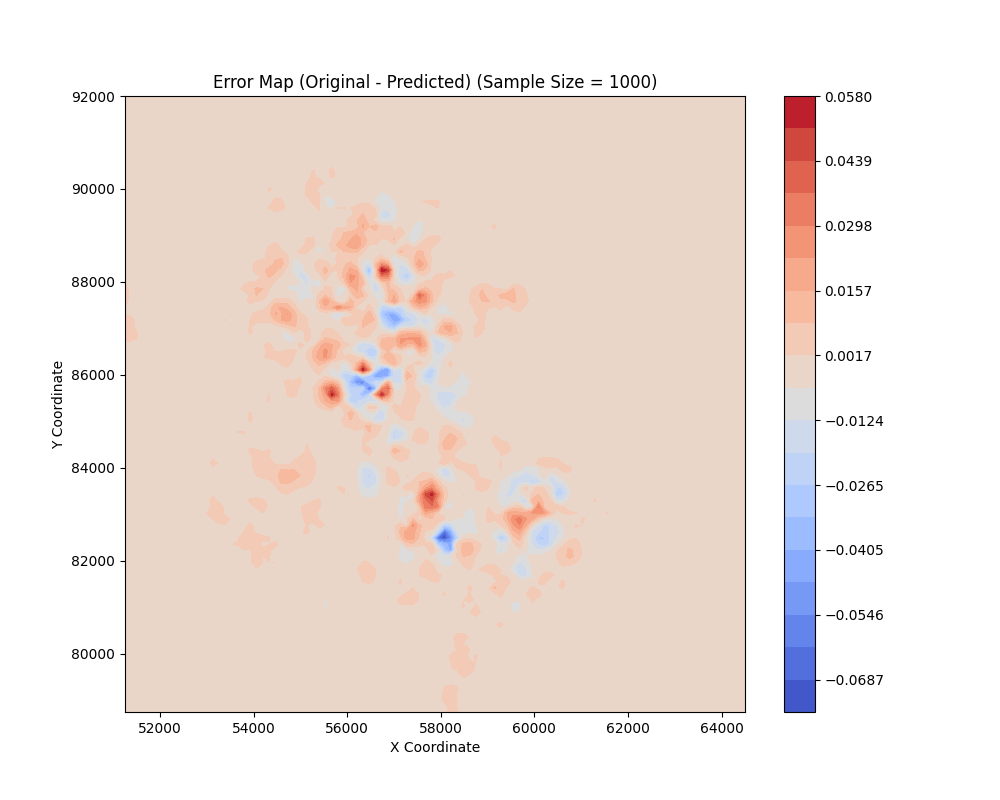
\includegraphics[width=0.3\linewidth]{Problem 3/Problem 3/Co-Kriging/Error_Map_Sample_Size_1000.png}}
\caption{Sample size 1000 results}
\end{figure}

\begin{figure}[h!t]
\centering
\subfigure[Predicted 50]{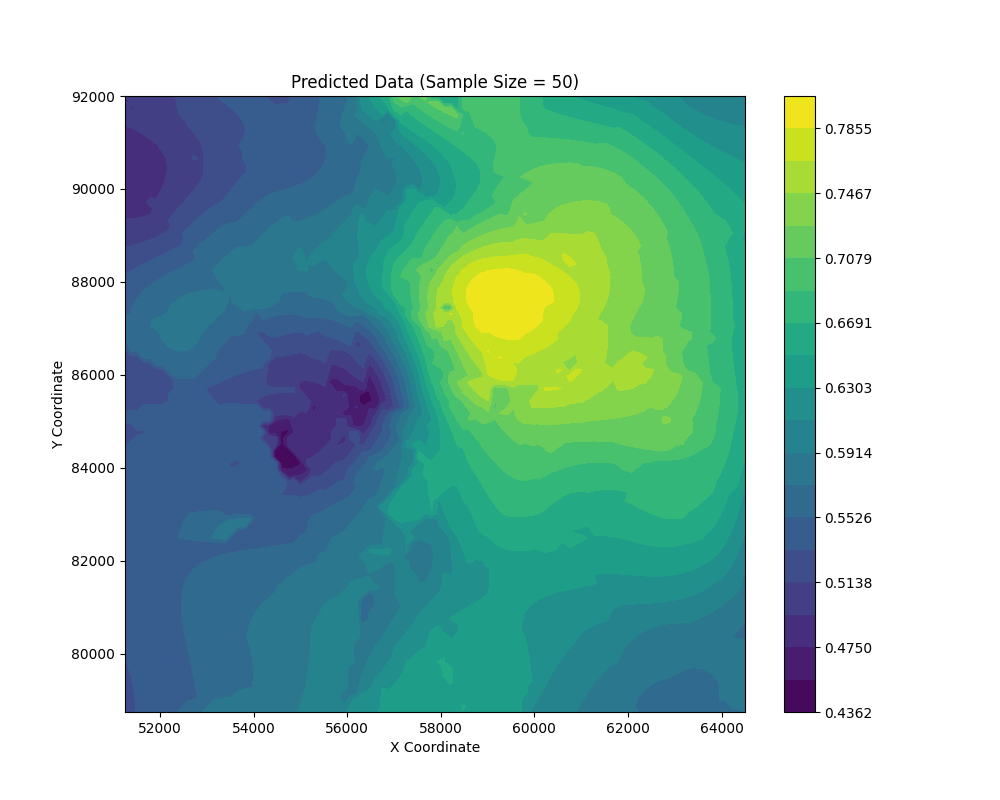
\includegraphics[width=0.23\linewidth]{Problem 3/Problem 3/Co-Kriging/Predicted_Data_Sample_Size_50.png}}
\subfigure[Error Map 50]{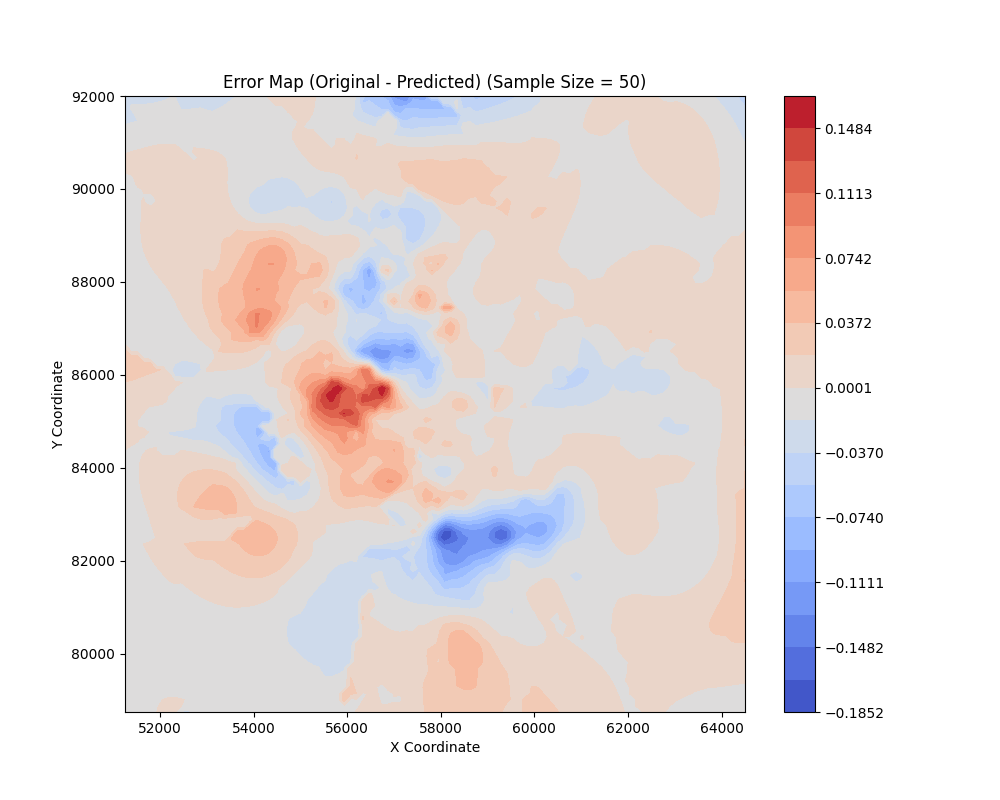
\includegraphics[width=0.23\linewidth]{Problem 3/Problem 3/Co-Kriging/Error_Map_Sample_Size_50.png}}
\subfigure[Predicted 200]{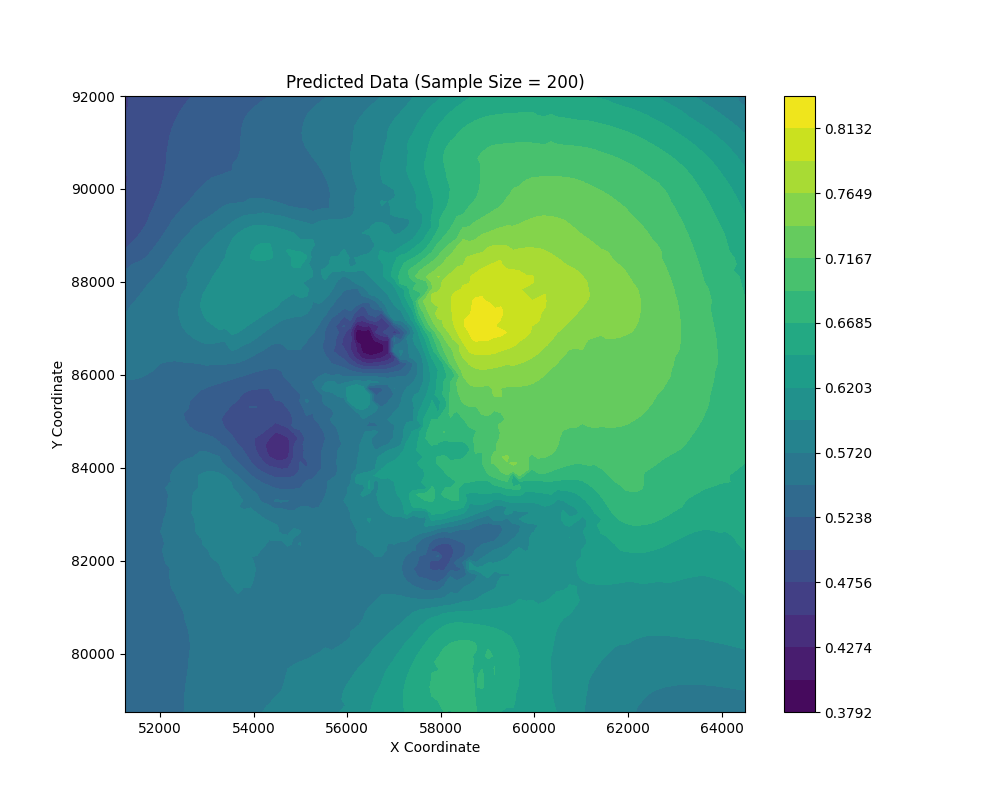
\includegraphics[width=0.23\linewidth]{Problem 3/Problem 3/Co-Kriging/Predicted_Data_Sample_Size_200.png}}
\subfigure[Error Map 200]{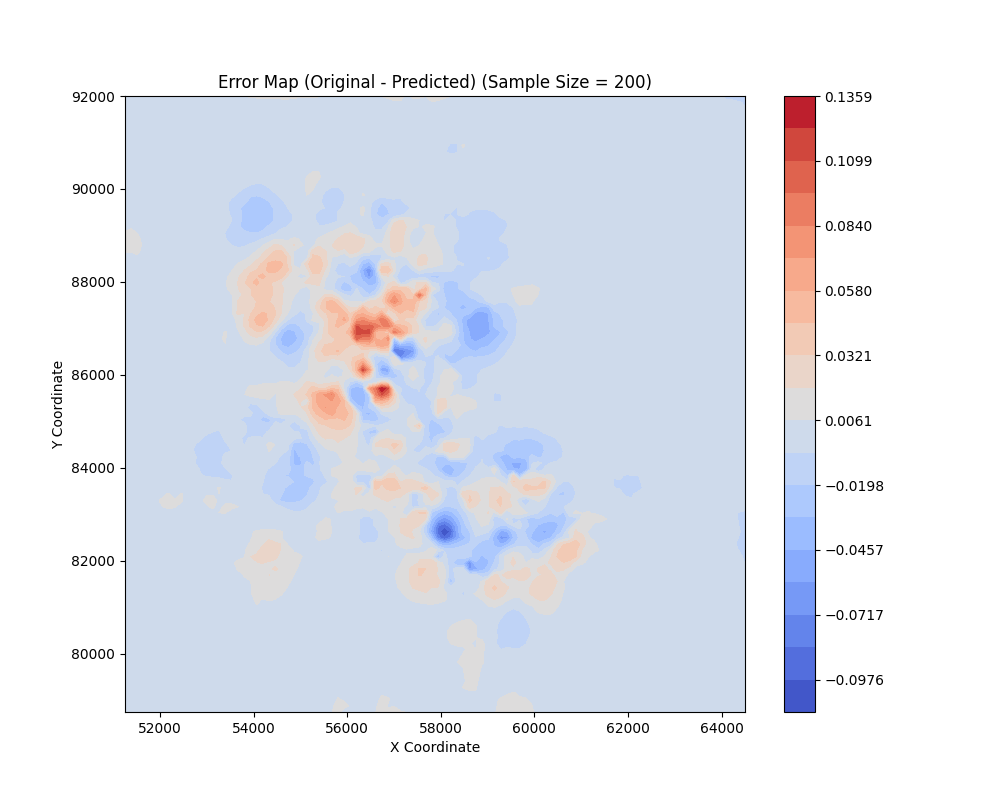
\includegraphics[width=0.23\linewidth]{Problem 3/Problem 3/Co-Kriging/Error_Map_Sample_Size_200.png}}

\subfigure[Predicted 500]{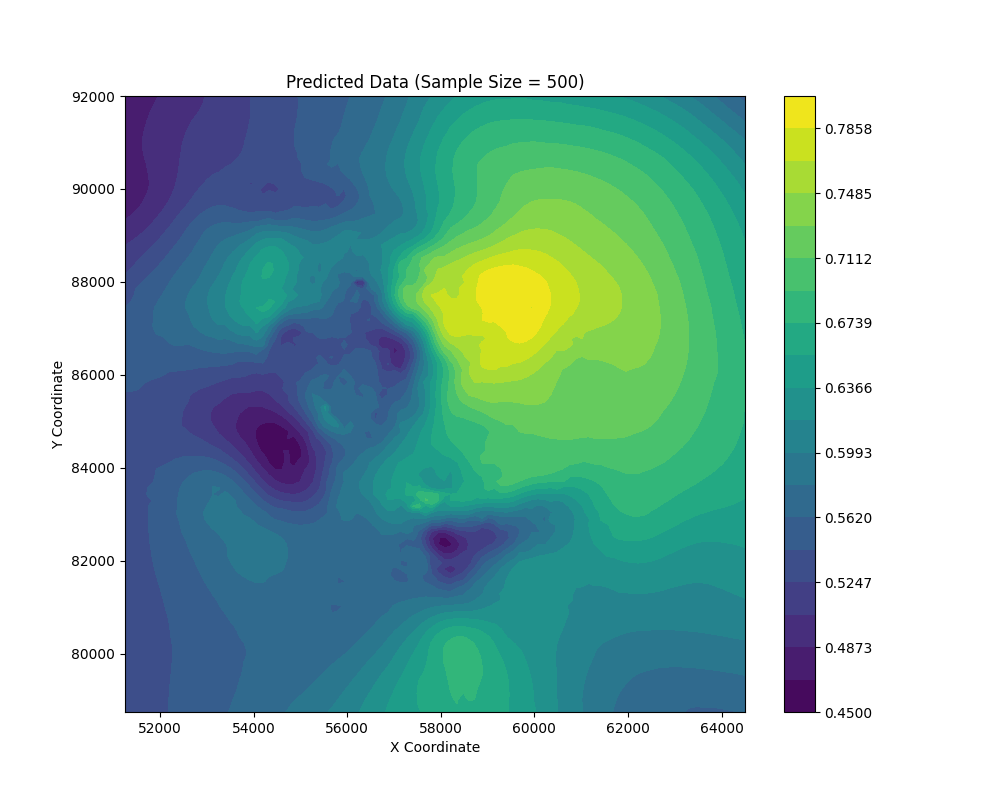
\includegraphics[width=0.23\linewidth]{Problem 3/Problem 3/Co-Kriging/Predicted_Data_Sample_Size_500.png}}
\subfigure[Error Map 500]{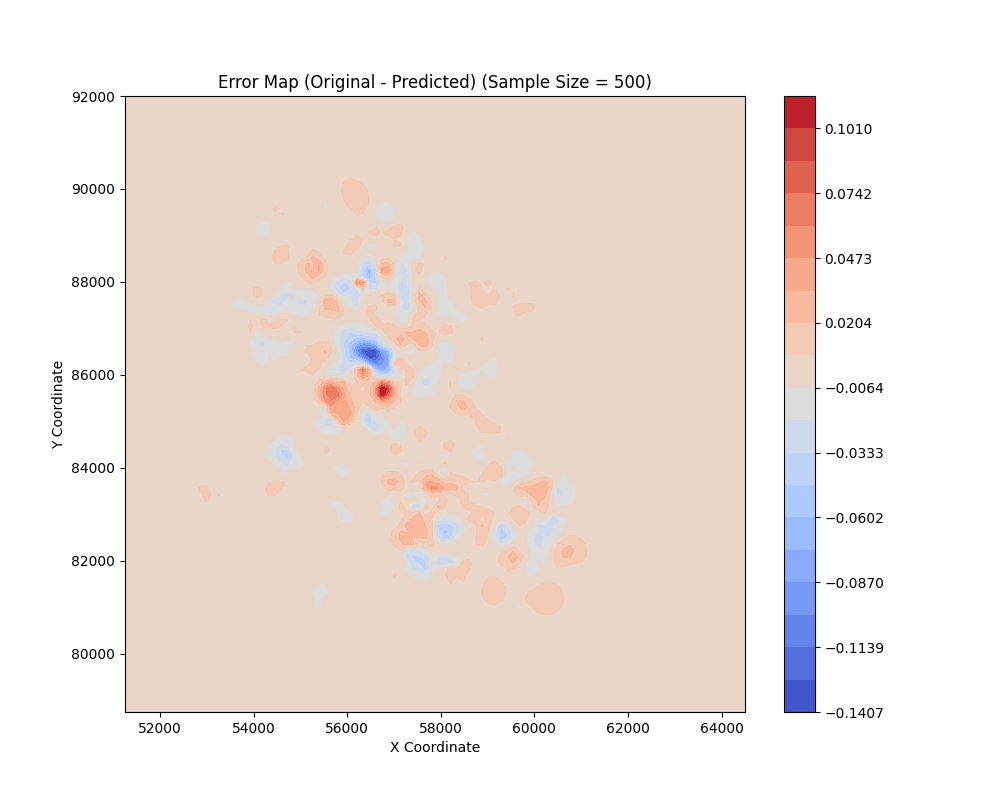
\includegraphics[width=0.23\linewidth]{Problem 3/Problem 3/Co-Kriging/Error_Map_Sample_Size_500.png}}
\subfigure[Predicted 8000]{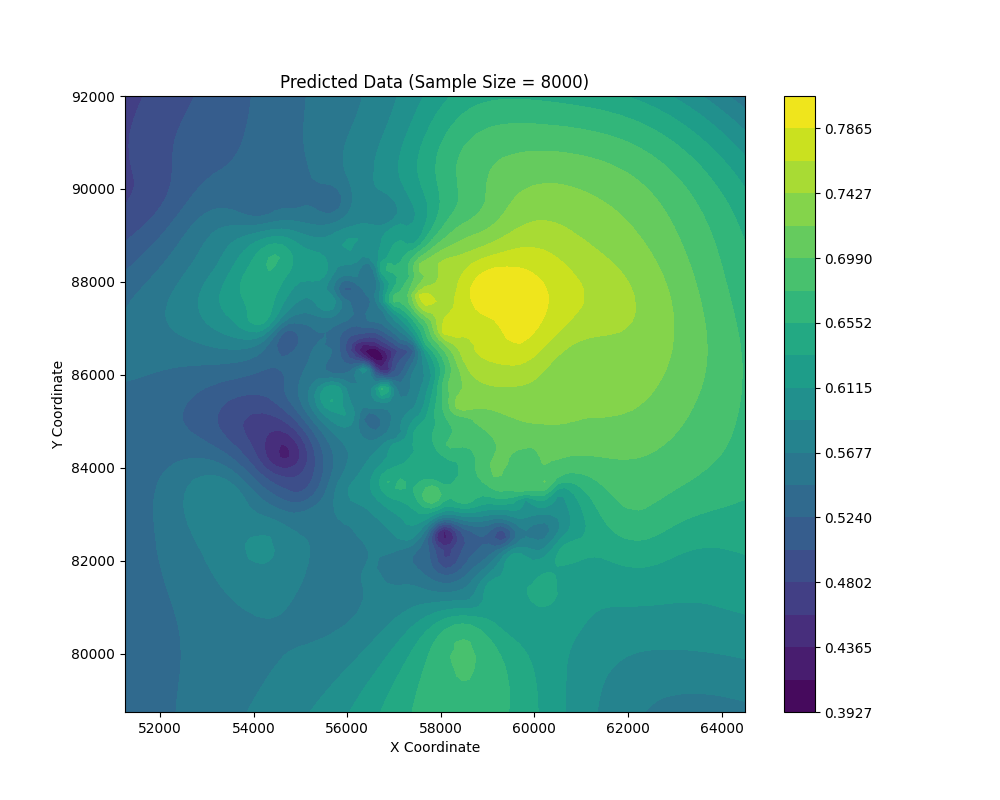
\includegraphics[width=0.23\linewidth]{Problem 3/Problem 3/Co-Kriging/Predicted_Data_Sample_Size_8000.png}}
\subfigure[Error Map 8000]{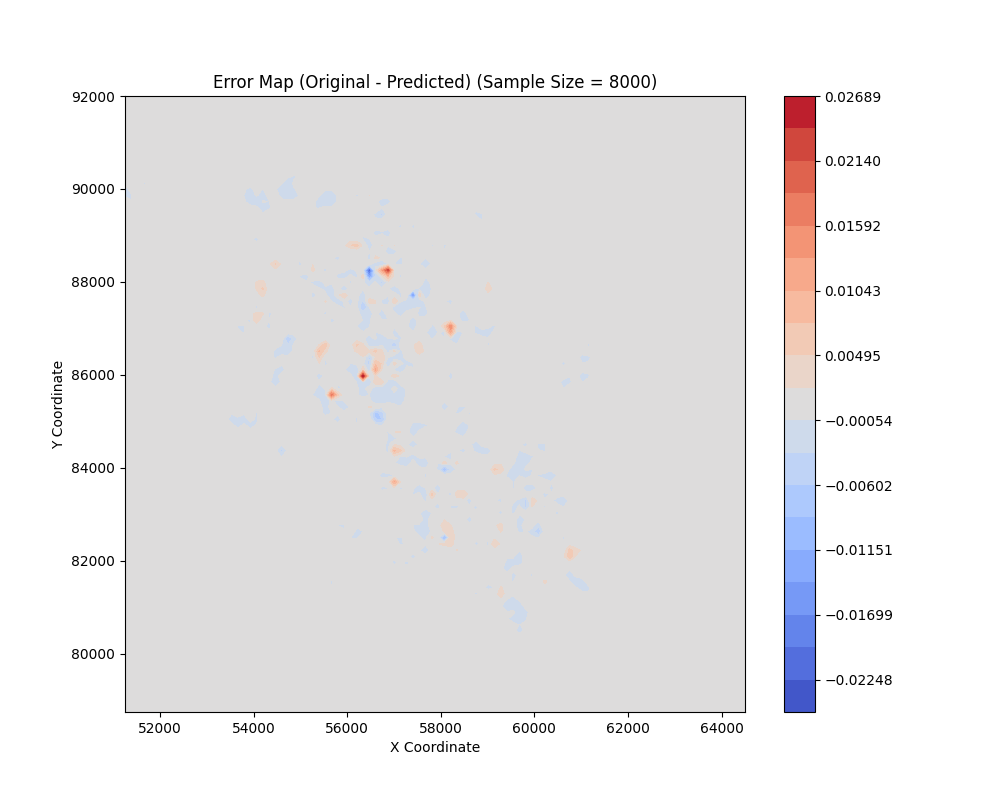
\includegraphics[width=0.23\linewidth]{Problem 3/Problem 3/Co-Kriging/Error_Map_Sample_Size_8000.png}}

\subfigure[Predicted 25000]{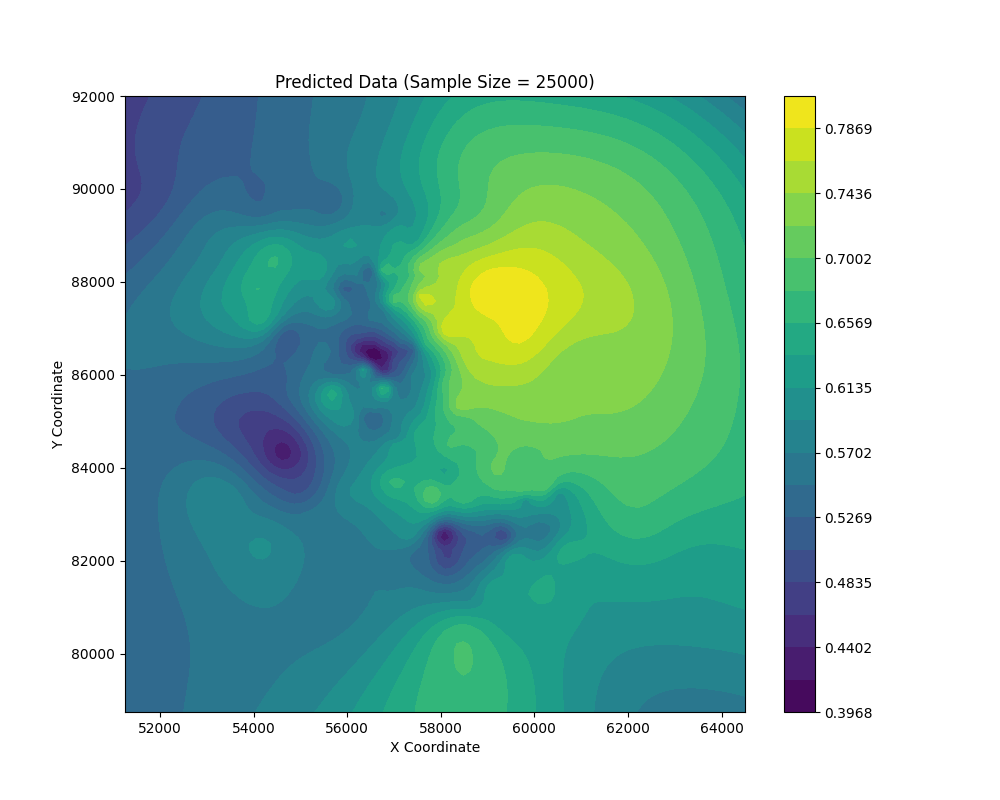
\includegraphics[width=0.23\linewidth]{Problem 3/Problem 3/Co-Kriging/Predicted_Data_Sample_Size_25000.png}}
\subfigure[Error Map 25000]{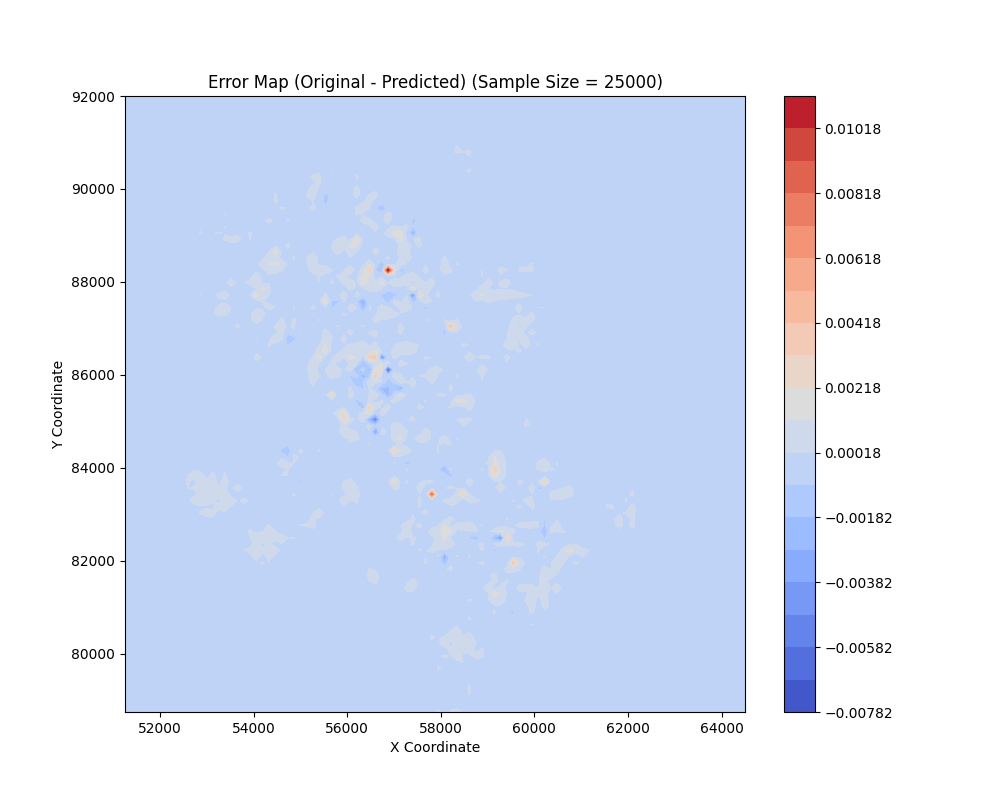
\includegraphics[width=0.23\linewidth]{Problem 3/Problem 3/Co-Kriging/Error_Map_Sample_Size_25000.png}}
\subfigure[Predicted 50000]{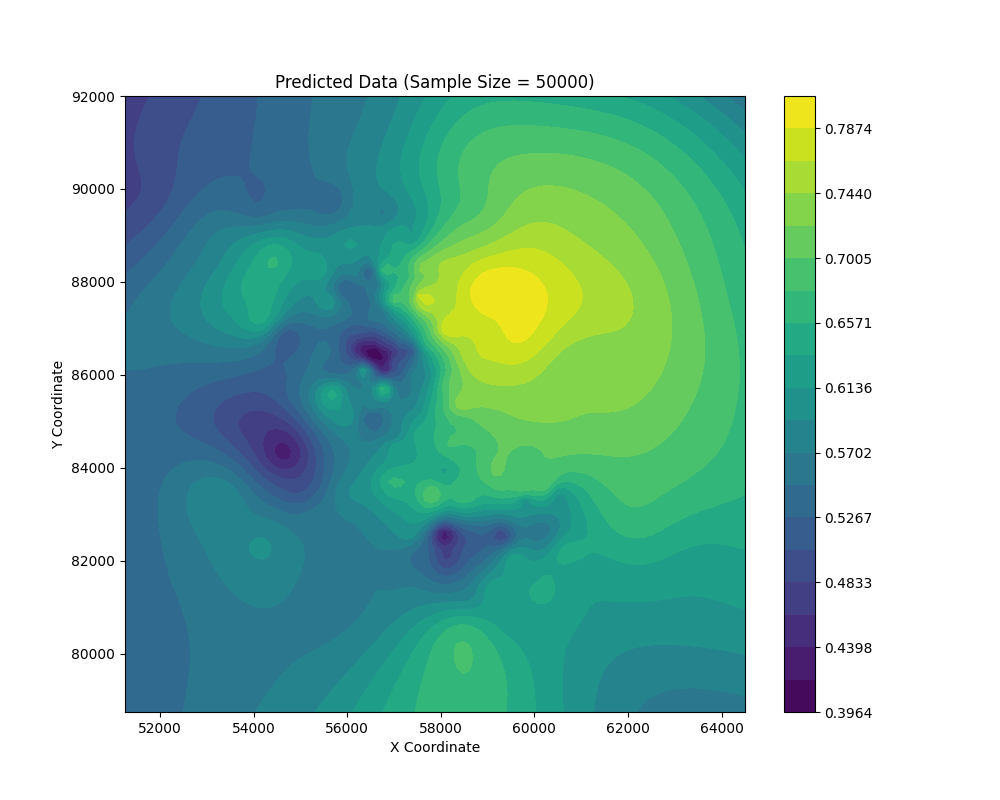
\includegraphics[width=0.23\linewidth]{Problem 3/Problem 3/Co-Kriging/Predicted_Data_Sample_Size_50000.png}}
\subfigure[Error Map 50000]{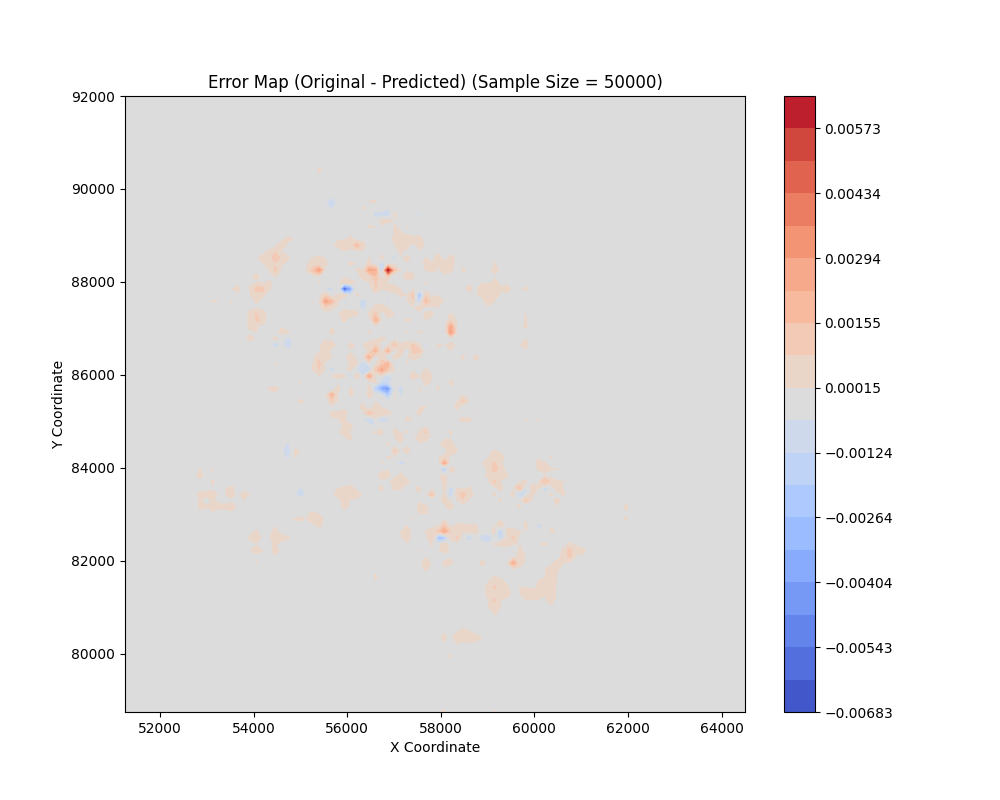
\includegraphics[width=0.23\linewidth]{Problem 3/Problem 3/Co-Kriging/Error_Map_Sample_Size_50000.png}}

\caption{Co-Kriging Results for Predicted Property and Error Maps at Different Sample Sizes}
\label{fig:all_samples_co_kriging}
\end{figure}

From the table, it is evident that as the sample size increases, the error metrics generally show a significant decreasing trend, indicating that larger data samples help improve the accuracy and reliability of the model. The characteristics remain consistent with those in table1.

\begin{table}[h!]
\centering
\caption{Co-Kriging Performance Metrics}
\label{tab:metrics}
\begin{tabular}{|c|c|c|c|c|}
\hline
\textbf{Sample Size} & \textbf{Percentage of Total} & \textbf{MSE} & \textbf{RMSE} & \textbf{MAE} \\ \hline
50     & 0.07\%  & 0.000766 & 0.027679 & 0.016712 \\ \hline
200    & 0.28\%  & 0.000168 & 0.012948 & 0.006117 \\ \hline
500    & 0.71\%  & 0.000068 & 0.008262 & 0.002826 \\ \hline
1000   & 1.41\%  & 0.000025 & 0.004984 & 0.001668 \\ \hline
8000   & 11.31\% & 0.000001 & 0.000853 & 0.000252 \\ \hline
25000  & 35.33\% & 0 & 0.000331 & 0.000106 \\ \hline
50000  & 70.67\% & 0 & 0.00226  & 0.000069 \\ \hline
\end{tabular}
\end{table}


\subsection{Machine Learning - SVM}
SVM is a powerful supervised learning method commonly used for classification and regression tasks \cite{bib8}. Folowing is the result with the steps similar to section 6.1.

\begin{figure}[h!t]
\centering
\subfigure[Predicted 50]{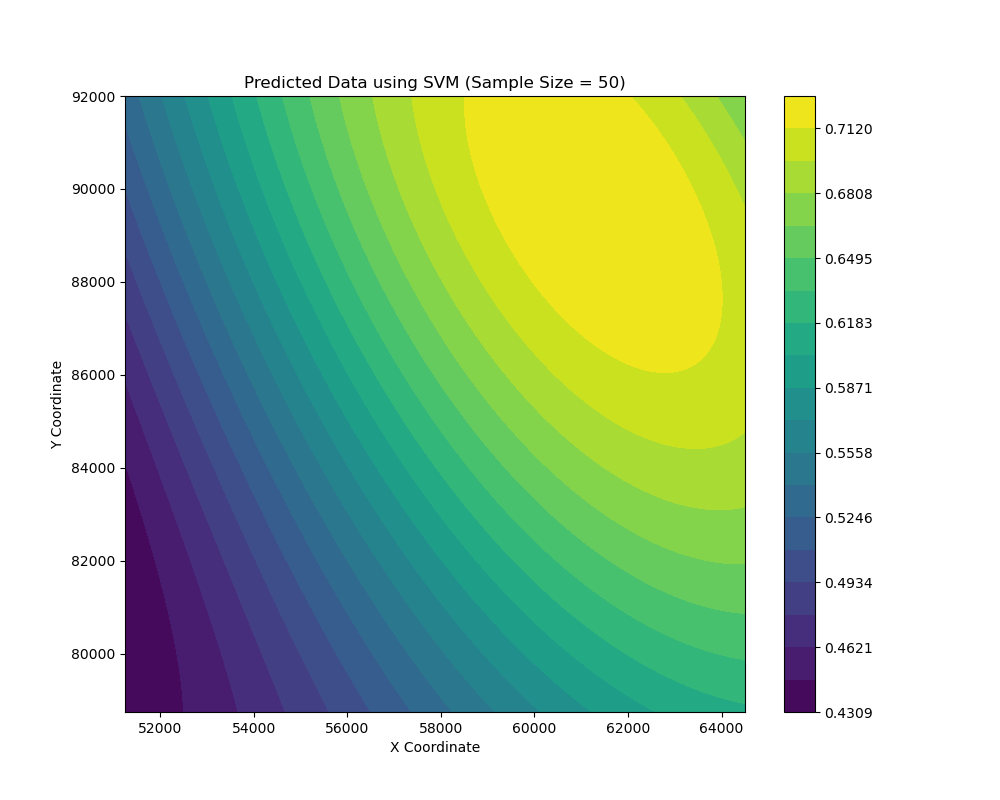
\includegraphics[width=0.23\linewidth]{Problem 3/Problem 3/SVM/Predicted_Data_SVM_Sample_Size_50.png}}
\subfigure[Error Map 50]{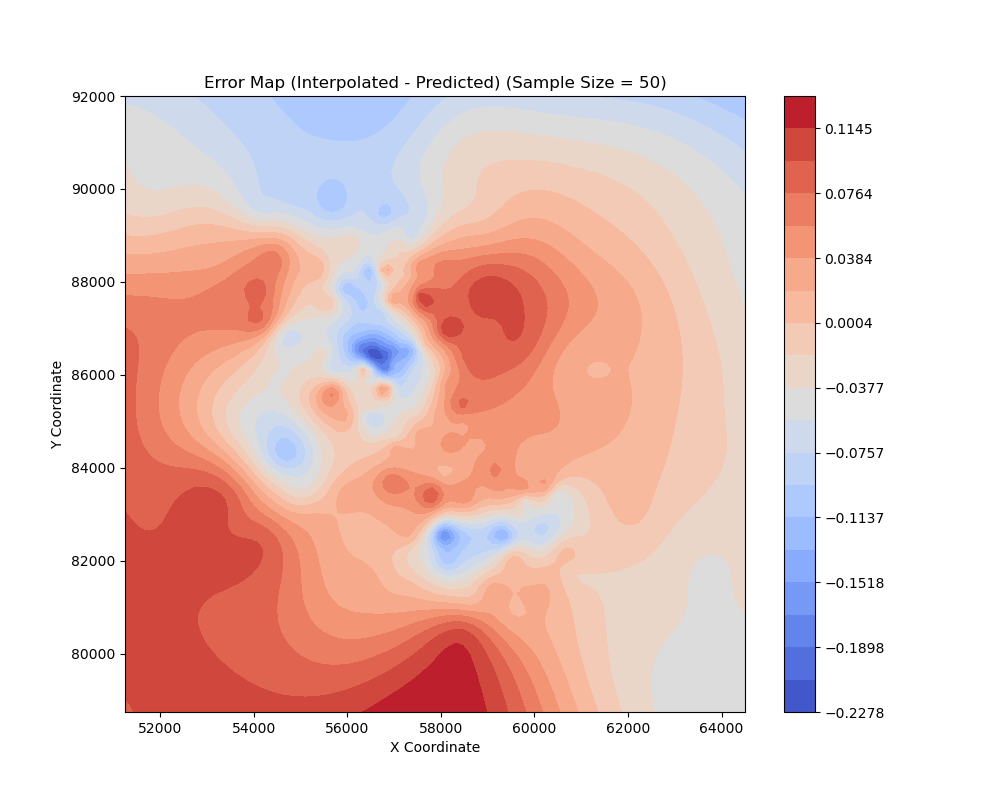
\includegraphics[width=0.23\linewidth]{Problem 3/Problem 3/SVM/Error_Map_SVM_Sample_Size_50.png}}
\subfigure[Predicted 200]{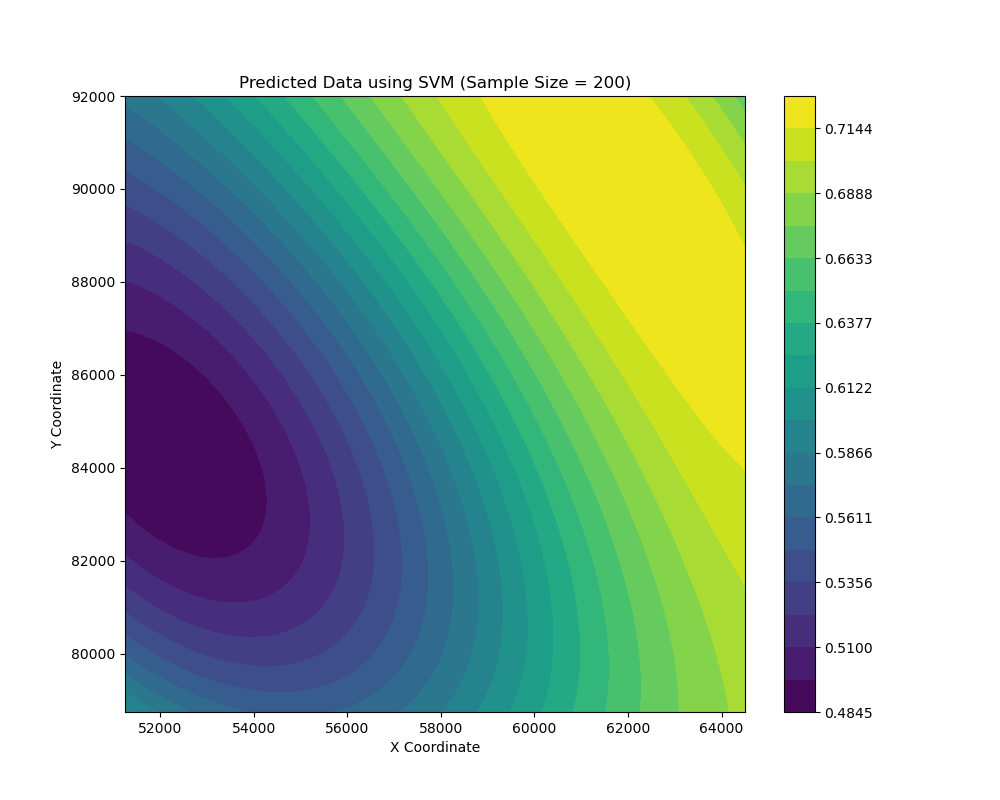
\includegraphics[width=0.23\linewidth]{Problem 3/Problem 3/SVM/Predicted_Data_SVM_Sample_Size_200.png}}
\subfigure[Error Map 200]{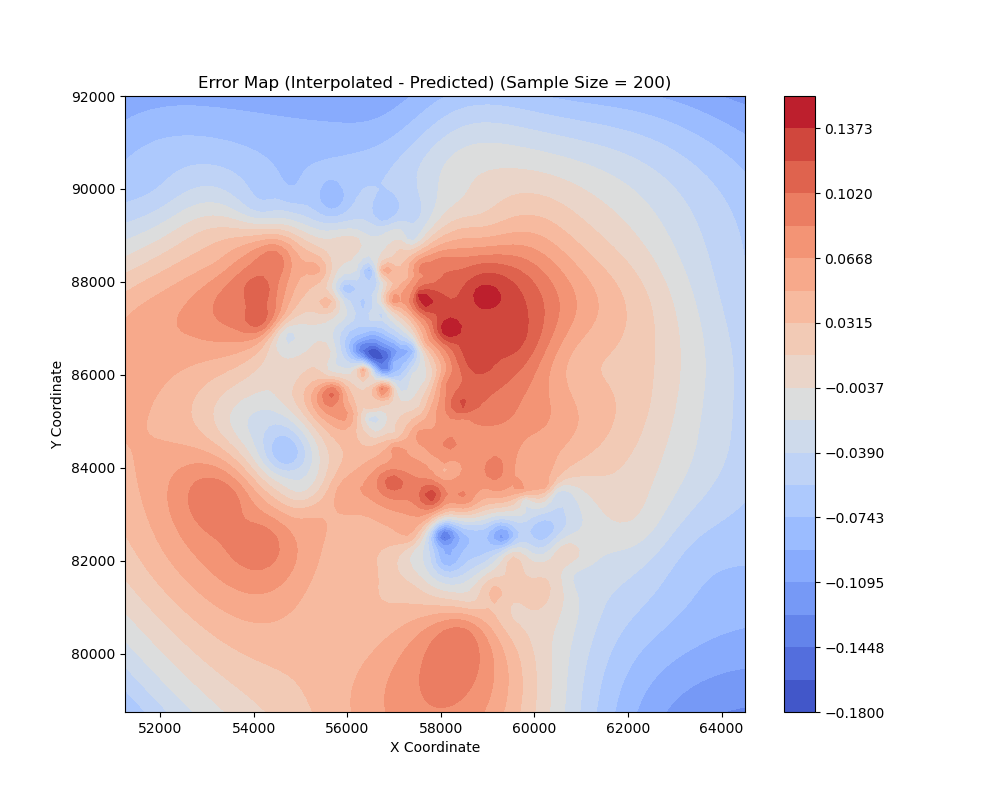
\includegraphics[width=0.23\linewidth]{Problem 3/Problem 3/SVM/Error_Map_SVM_Sample_Size_200.png}}

\subfigure[Predicted 500]{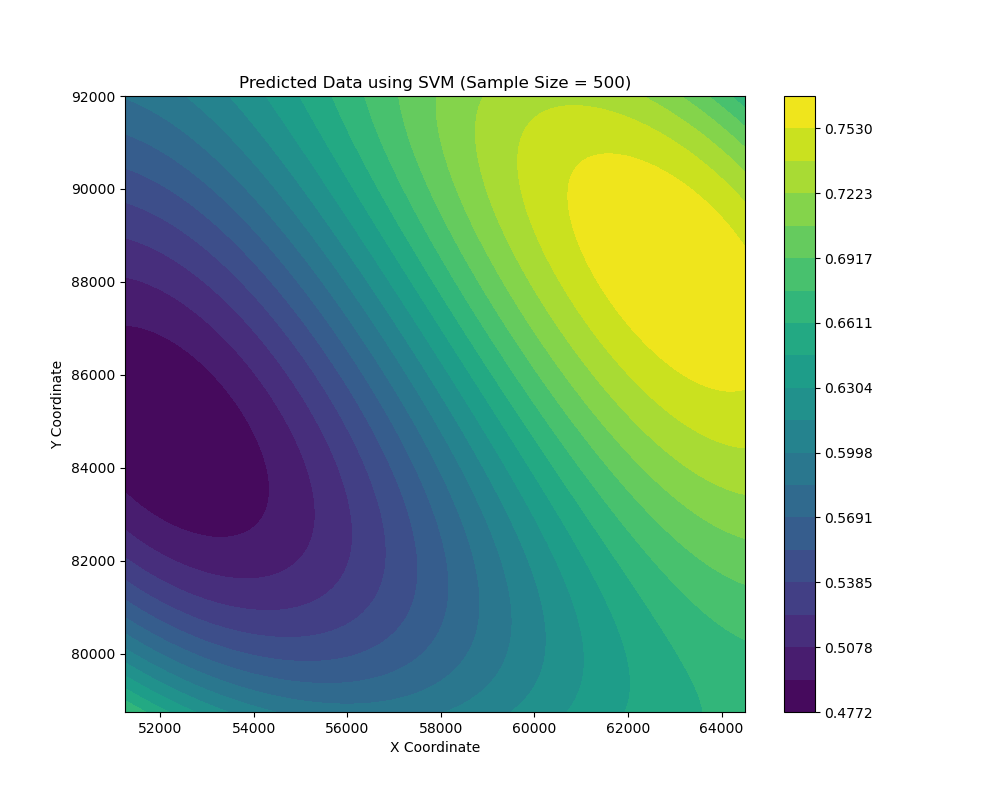
\includegraphics[width=0.23\linewidth]{Problem 3/Problem 3/SVM/Predicted_Data_SVM_Sample_Size_500.png}}
\subfigure[Error Map 500]{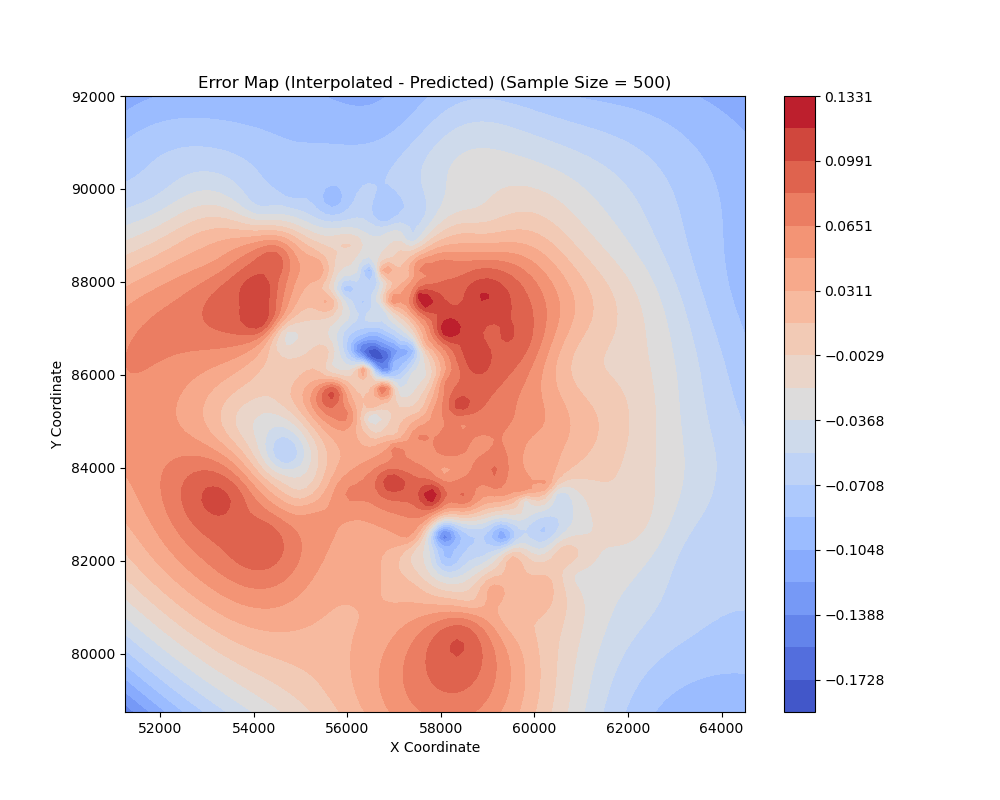
\includegraphics[width=0.23\linewidth]{Problem 3/Problem 3/SVM/Error_Map_SVM_Sample_Size_500.png}}
\subfigure[Predicted 8000]{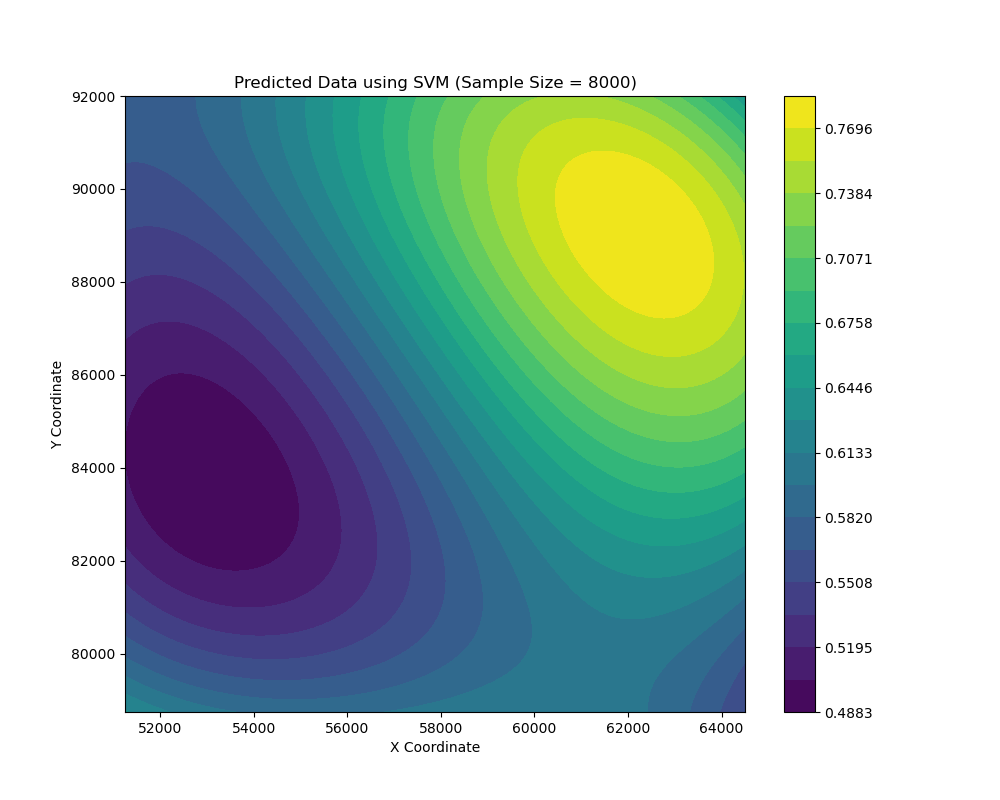
\includegraphics[width=0.23\linewidth]{Problem 3/Problem 3/SVM/Predicted_Data_SVM_Sample_Size_8000.png}}
\subfigure[Error Map 8000]{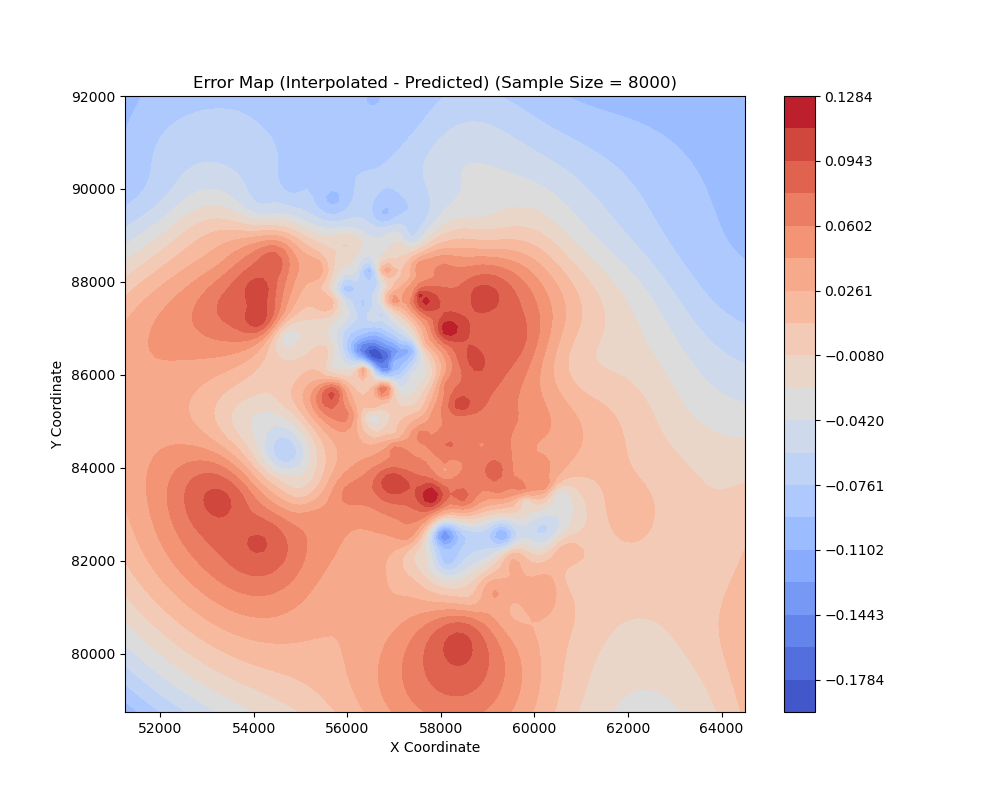
\includegraphics[width=0.23\linewidth]{Problem 3/Problem 3/SVM/Error_Map_SVM_Sample_Size_8000.png}}

\subfigure[Predicted 25000]{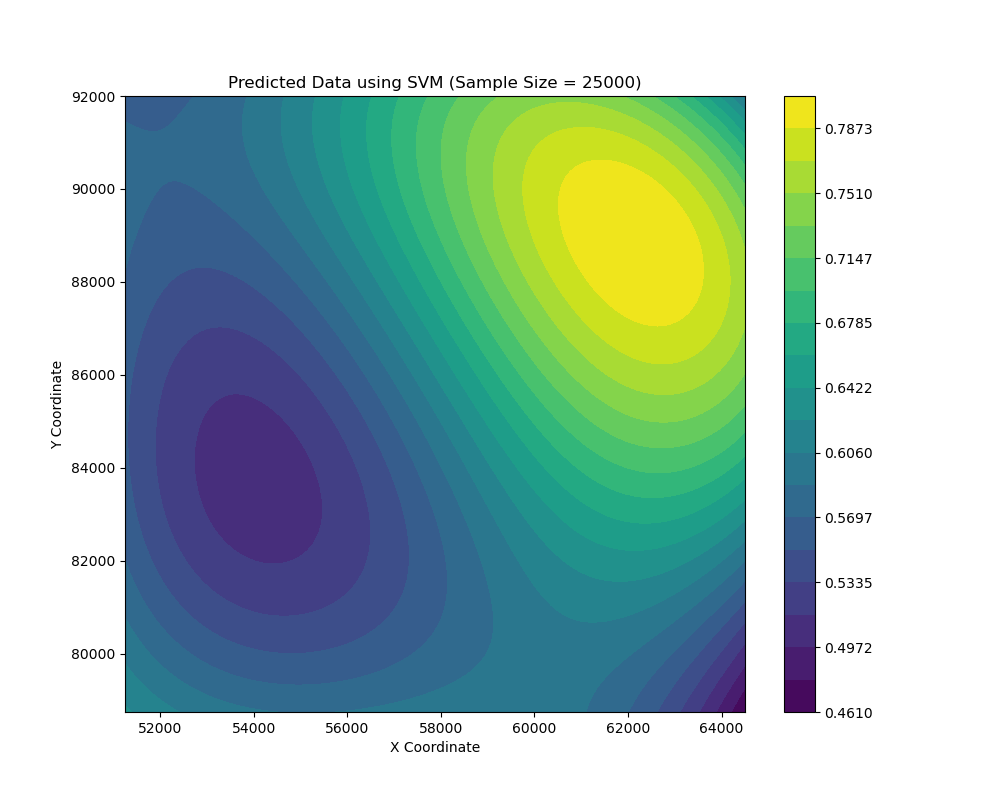
\includegraphics[width=0.23\linewidth]{Problem 3/Problem 3/SVM/Predicted_Data_SVM_Sample_Size_25000.png}}
\subfigure[Error Map 25000]{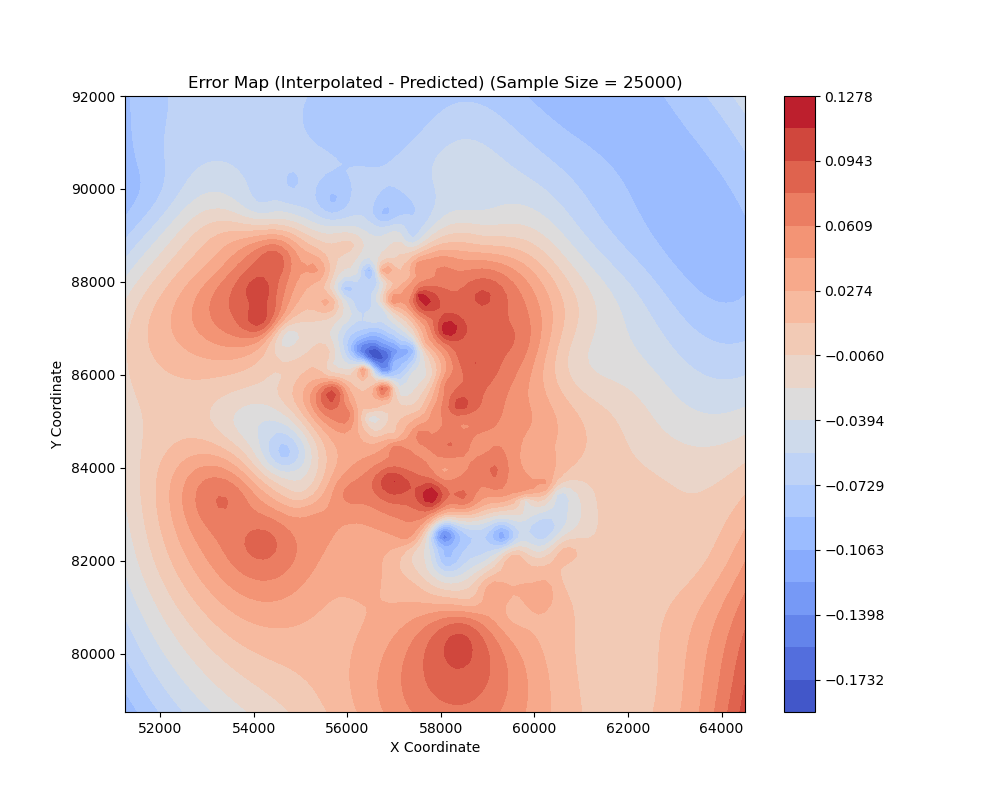
\includegraphics[width=0.23\linewidth]{Problem 3/Problem 3/SVM/Error_Map_SVM_Sample_Size_25000.png}}
\subfigure[Predicted 50000]{\includegraphics[width=0.23\linewidth]{Problem 3/Problem 3/SVM/Predicted_Data_SVM_Sample_Size_50000.png}}
\subfigure[Error Map 50000]{\includegraphics[width=0.23\linewidth]{Problem 3/Problem 3/SVM/Error_Map_SVM_Sample_Size_50000.png}}

\caption{SVM Results for Predicted Property and Error Maps at Different Sample Sizes}
\label{fig:all_results}
\end{figure}

The table presents the performance metrics (MSE, RMSE, MAE) for different sample sizes when using the Support Vector Machine (SVM) method. As shown in Table 4, even though the metrics such as MSE and RMSE appear to stabilize with increasing sample sizes—from 0.003576 at 50 samples to 0.002924 at 50,000 samples—the overall performance is still unsatisfactory. The MAE remains significantly high across all sample sizes, only slightly improving from 0.049833 at 50 samples to 0.045339 at 50,000 samples. This pattern indicates that while SVM is adept at handling nonlinear problems in low-dimensional features, it struggles in this case to effectively capture the necessary features, resulting in consistently high error rates. This suggests that SVM may not be the most suitable method for solving this problem, given its inability to adequately reduce error rates even as sample sizes increase significantly.

\begin{table}[h!]
\centering
\caption{SVM Performance Metrics}
\label{tab:metrics_update}
\begin{tabular}{|c|c|c|c|c|}
\hline
\textbf{Sample Size} & \textbf{Percentage of Total} & \textbf{MSE} & \textbf{RMSE} & \textbf{MAE} \\ \hline
50     & 0.07\%  & 0.003576 & 0.059803 & 0.049833 \\ \hline
200    & 0.28\%  & 0.003042 & 0.058477 & 0.049527 \\ \hline
500    & 0.71\%  & 0.003049 & 0.059077 & 0.051133 \\ \hline
1000   & 1.41\%  & 0.003407 & 0.058368 & 0.050837 \\ \hline
8000   & 11.31\% & 0.002914 & 0.053986 & 0.044774 \\ \hline
25000  & 35.33\% & 0.002917 & 0.054009 & 0.044643 \\ \hline
50000  & 70.67\% & 0.002924 & 0.054219 & 0.045339 \\ \hline
\end{tabular}
\end{table}

\subsection{Regression Kriging}

Regression Kriging combines the strengths of regression and kriging, making it a hybrid geostatistical technique. The regression component identifies and models global trends in the data, while the kriging component captures and interpolates the localized spatial variability. Following the similar steps and process as in Section 6.1, using the Regression Kriging algorithm, we obtained different results, with the corresponding contour maps and the error map shown below:

\begin{figure}[h!t]
\centering
\subfigure[Predicted Property 1000]{\includegraphics[width=0.3\linewidth]{Problem 3/Problem 3/Regression_Kriging/Regression_Predicted_Data_Sample_Size_1000.png}}\hfill
\subfigure[Original Property]{\includegraphics[width=0.3\linewidth]{Problem 1/Problem 1/Original_Data_Points.png}}\hfill
\subfigure[Error Map 1000]{\includegraphics[width=0.3\linewidth]{Problem 3/Problem 3/Regression_Kriging/Regression_Error_Map_Sample_Size_1000.png}}
\caption{Sample size 1000 results using Regression Kriging}
\end{figure}

\begin{figure}[h!t]
\centering
\subfigure[Predicted 50]{\includegraphics[width=0.23\linewidth]{Problem 3/Problem 3/Regression_Kriging/Regression_Predicted_Data_Sample_Size_50.png}}
\subfigure[Error Map 50]{\includegraphics[width=0.23\linewidth]{Problem 3/Problem 3/Regression_Kriging/Regression_Error_Map_Sample_Size_50.png}}
\subfigure[Predicted 200]{\includegraphics[width=0.23\linewidth]{Problem 3/Problem 3/Regression_Kriging/Regression_Predicted_Data_Sample_Size_200.png}}
\subfigure[Error Map 200]{\includegraphics[width=0.23\linewidth]{Problem 3/Problem 3/Regression_Kriging/Regression_Error_Map_Sample_Size_200.png}}

\subfigure[Predicted 500]{\includegraphics[width=0.23\linewidth]{Problem 3/Problem 3/Regression_Kriging/Regression_Predicted_Data_Sample_Size_500.png}}
\subfigure[Error Map 500]{\includegraphics[width=0.23\linewidth]{Problem 3/Problem 3/Regression_Kriging/Regression_Error_Map_Sample_Size_500.png}}
\subfigure[Predicted 8000]{\includegraphics[width=0.23\linewidth]{Problem 3/Problem 3/Regression_Kriging/Regression_Predicted_Data_Sample_Size_8000.png}}
\subfigure[Error Map 8000]{\includegraphics[width=0.23\linewidth]{Problem 3/Problem 3/Regression_Kriging/Regression_Error_Map_Sample_Size_8000.png}}

\subfigure[Predicted 25000]{\includegraphics[width=0.23\linewidth]{Problem 3/Problem 3/Regression_Kriging/Regression_Predicted_Data_Sample_Size_25000.png}}
\subfigure[Error Map 25000]{\includegraphics[width=0.23\linewidth]{Problem 3/Problem 3/Regression_Kriging/Regression_Error_Map_Sample_Size_25000.png}}
\subfigure[Predicted 50000]{\includegraphics[width=0.23\linewidth]{Problem 3/Problem 3/Regression_Kriging/Regression_Predicted_Data_Sample_Size_50000.png}}
\subfigure[Error Map 50000]{\includegraphics[width=0.23\linewidth]{Problem 3/Problem 3/Regression_Kriging/Regression_Error_Map_Sample_Size_50000.png}}

\caption{Regression Kriging Results for Predicted Property and Error Maps}
\label{fig:comprehensive_regression_kriging_results}
\end{figure}

\vspace{10em}

The following table presents the Regression Kriging performance metrics, derived from the contour maps and error map shown above. These metrics include Mean Squared Error (MSE), Root Mean Squared Error (RMSE), and Mean Absolute Error (MAE), all evaluated at different sample sizes, following the same structure as Table 3. The results highlight the effectiveness of the Regression Kriging algorithm in spatial prediction tasks.

\begin{table}[h!]
\centering
\caption{Regression Kriging Performance Metrics}
\label{tab:metrics}
\begin{tabular}{|c|c|c|c|c|}
\hline
\textbf{Sample Size} & \textbf{Percentage of Total} & \textbf{MSE} & \textbf{RMSE} & \textbf{MAE} \\ \hline
50     & 0.07\%  & 0.000067 & 0.025882 & 0.016659 \\ \hline
200    & 0.28\%  & 0.000284 & 0.016865 & 0.007641 \\ \hline
500    & 0.71\%  & 0.000068 & 0.008242 & 0.003043 \\ \hline
1000   & 1.41\%  & 0.000026 & 0.005129 & 0.001735 \\ \hline
8000   & 11.31\% & 0.000001 & 0.001029 & 0.000256 \\ \hline
25000  & 35.33\% & 0 & 0.000359 & 0.000108 \\ \hline
50000  & 70.67\% & 0 & 0.000222 & 0.000069 \\ \hline
\end{tabular}
\end{table}


\subsection{Comparison}

Building on the results from the earlier analysis, we decide to exclude the SVM method from further consideration due to its relatively lower performance in this context. With SVM removed, the focus shifts to a comparative analysis between Co-Kriging and Regression Kriging. To facilitate this comparison, we perform a subtraction operation on the metrics presented in Table 3 and Table 5. This operation allows us to directly quantify the differences in performance between the two methods, providing a clearer assessment of their relative strengths and weaknesses.

\begin{table}[h!]
\centering
\caption{Regression Kriging minus Co-Kriging}
\begin{tabular}{|c|c|c|c|}
\hline
\textbf{Sample Size} & \textbf{MSE} & \textbf{RMSE} & \textbf{MAE} \\\hline
50     & -0.000096 & -0.0018 & -0.000053 \\\hline
200    &0.000116 & 0.003917 & 0.001524 \\\hline
500    &0.000000 & -0.00002 & 0.000217 \\\hline
1000   &0.000001 & 0.000145 & 0.000067 \\\hline
8000   &0.000000 & 0.000176 & 0.000004 \\\hline
25000  &0.000000 & 0.000028 & 0.000002 \\\hline
50000  &0.000000 & -0.00004 & 0.000000 \\\hline
\end{tabular}
\end{table}

Next, the performance of the two algorithms are analyzed. If the difference in the metric values is positive, it indicates that Regression Kriging performs worse. If the difference is negative, it indicates that Regression Kriging performs better. If the difference is zero, it is considered a tie. The results are summarized in the following table:

\begin{table}[h!]
\centering
\caption{Comparison of Wins Between Regression Kriging and Co-Kriging}
\begin{tabular}{|c|c|c|c|}
\hline
\textbf{Metric} & \textbf{Co-Kriging Wins} & \textbf{Regression Kriging Wins} & \textbf{Ties} \\\hline
MSE             & 2                                & 1                        & 4            \\\hline
RMSE            & 4                               & 3                        & 0            \\\hline
MAE             & 5                                & 1                        & 1            \\\hline
\end{tabular}
\end{table}

From the analysis of the table, it can be observed that Co-Kriging generally outperforms Regression Kriging. Specifically, Co-Kriging wins in 2 cases for MSE, compared to 1 win for Regression Kriging, with 4 ties. For RMSE, Co-Kriging wins 4 times, while Regression Kriging wins 3 times, with no ties. For MAE, Co-Kriging achieves 5 wins against 1 for Regression Kriging, with 1 tie. These results suggest that Co-Kriging provides slightly better predictive accuracy. However, Regression Kriging still shows competitive performance in certain instances, particularly with RMSE, where the gap between the two methods is narrower.


\section{Problem 4}

To begin the analysis, we generate a distribution map with 1,000 data points from the F2 dataset. The primary goal is to ensure that these data points are randomly sampled across the entire study area, avoiding any undue concentration in specific regions. This random sampling process is critical for maintaining spatial balance and ensuring no area disproportionately influences the results. Upon examining the distribution map, we find that the data points are uniformly spread across the spatial domain. This even distribution meets the requirement for randomness and spatial coverage, ensuring the robustness and reliability of subsequent analyses based on this dataset.

\begin{figure}[h!t]
	\centering
	\includegraphics[width=0.8\textwidth]{Problem 4/Problem 4/F2_Original_Data_Points.png}
	\caption{F2\_Original\_Data\_Points}
\end{figure}

Using the most suitable algorithm determined in Question 3, which is Co-Kriging, a predictive map illustrating the distribution of the target variable for the F2 dataset is generated. This map is created with the aid of the 1000 sample data provided in the target file along with the four additional collaborative variables files.



\begin{figure}[h!t]
	\centering
	\includegraphics[width=0.8\textwidth]{Problem 4/Problem 4/F2_Predicted_Data_Full_Data.png}
	\caption{F2\_Predicted\_Data}
\end{figure}


\newpage

\section{Conclusion}

This study successfully applies the Kriging algorithm for spatial analysis across different sample sizes, generating both predictive and error maps in the process. The results demonstrate that the accuracy of predictions improves significantly with increasing sample size, as reflected in the decreasing error metrics (MSE, RMSE, and MAE). Additionally, we use Spearman’s rank correlation coefficient to analyze the relationship between collaborative variables and the target variable. Collaborative variables with high correlations are then introduced to further optimize the performance of the prediction model using Kriging variants such as Co-Kriging and Regression Kriging, accelerated by cKDTree. By comparing the outcomes of different methodologies, the study shows that Co-Kriging and Regression Kriging yield more accurate predictions when dealing with complex datasets containing multiple correlated variables. However, the SVM algorithm proves less effective for prediction in this context, suggesting that it may not be suitable for the data or predictive tasks addressed in this study. This analysis offers an important academic insight: not all advanced machine learning techniques are applicable to all geostatistical problems. Overall, this research not only demonstrates the application of geostatistical methods in spatial data analysis but also examines the applicability and limitations of various techniques, providing valuable insights and references for future research.

%----------------------------参考文献
\newpage

\begin{thebibliography}{9}%宽度9
\bibitem{bib1} \url{https://www.paulamoraga.com/book-spatial/kriging.html}
\bibitem{bib2} \url{https://statistics.laerd.com/statistical-guides/spearmans-rank-order-correlation-statistical-guide.php}
\bibitem{bib3} \url{https://support.minitab.com/minitab/help-and-how-to/statistics/basic-statistics/supporting-topics/correlation-and-covariance/a-comparison-of-the-pearson-and-spearman-correlation-methods/}

\bibitem{bib4} Akash Anand, Prachi Singh, Prashant K. Srivastava, Manika Gupta,
Chapter 19 - GIS-based analysis for soil moisture estimation via kriging with external drift,
Editor(s): Prashant K. Srivastava, Manika Gupta, George Tsakiris, Nevil Wyndham Quinn,
Agricultural Water Management,
Academic Press,
2021,
Pages 391-408,
ISBN 9780128123621,
\url{https://doi.org/10.1016/B978-0-12-812362-1.00019-9.}

\bibitem{bib5} M.A. Oliver, R. Webster,
A tutorial guide to geostatistics: Computing and modelling variograms and kriging,
CATENA,
Volume 113,
2014,
Pages 56-69,
ISSN 0341-8162,
\url{https://doi.org/10.1016/j.catena.2013.09.006.}

\bibitem{bib6} M.K. Borregaard, D.K. Hendrichsen, G. Nachman,
Spatial Distribution,
Editor(s): Sven Erik Jørgensen, Brian D. Fath,
Encyclopedia of Ecology,
Academic Press,
2008,
Pages 3304-3310,
ISBN 9780080454054,
\url{https://doi.org/10.1016/B978-008045405-4.00659-5.}

\bibitem{bib7} James R Carr, Donald E Myers, Charles E Glass,
Cokriging—a computer program,
Computers \& Geosciences,
Volume 11, Issue 2,
1985,
Pages 111-127,
ISSN 0098-3004,
\url{https://doi.org/10.1016/0098-3004(85)90002-0.}

\bibitem{bib8} Du, P., Bai, X., Tan, K. et al. Advances of Four Machine Learning Methods for Spatial Data Handling: a Review. J geovis spat anal 4, 13 (2020). \url{https://doi.org/10.1007/s41651-020-00048-5}

\bibitem{bib9} Erdogan Erten, Gamze \& Yavuz, Mahmut \& Deutsch, Clayton. (2022). Combination of Machine Learning and Kriging for Spatial Estimation of Geological Attributes. Natural Resources Research. 31. 10.1007/s11053-021-10003-w. 



\end{thebibliography}

% ---------------------开始附录

\newpage

\section*{Appendix}
% 在目录中添加Appendix
\addcontentsline{toc}{section}{Appendix}

\begin{lstlisting}[language=python,caption={The python programme for txt to csv and ploting for heatmaps }]

import numpy as np

with open('F1_target_variable.txt', 'r') as file:
    lines = file.readlines()

data = []
for line in lines:
    numbers = line.split()
    
    
    try:
        data.extend(map(float, numbers)) 
    except ValueError:
    
        continue

data_matrix = np.array(data).reshape(266, 266)

np.savetxt('F1_target_variable_grid.csv', data_matrix, delimiter=',', fmt='%.4f')

data_matrix = np.loadtxt('F1_target_variable_grid.csv', delimiter=',')

rows, cols = data_matrix.shape

x_coords, y_coords = np.meshgrid(range(cols), range(rows))

Column_Sequence = x_coords.flatten()
Row_Sequence = y_coords.flatten()
X_coordinate = y_coords.flatten()*50+51250
Y_coordinate = x_coords.flatten()*50+78750
values = data_matrix.flatten()

result = np.vstack((Column_Sequence,Row_Sequence, X_coordinate, Y_coordinate, values)).T

np.savetxt('F1_target_variable.csv', result, delimiter=',', header='Column Sequence,Row Sequence,X_Coordinate,Y_Coordinate,Target Property', fmt='%d, %d,%d, %d, %.4f', comments='')

fig, axes = plt.subplots(2, 2, figsize=(15, 12))  # Adjust the size of the subplots

for ax, file_name in zip(axes.flatten(), file_names):
    data = pd.read_csv('E:/2024ShuWei__B_Problem/Attachment 1/' + file_name)
    
    # Data preprocessing
    data = data.dropna()
    
    # Pivot data into matrix form for heatmap visualization
    heatmap_data = data.pivot(index='Row Sequence', columns='Column Sequence', values='Target Property')
    
    # Draw the heatmap
    sns.heatmap(heatmap_data, cmap='coolwarm', cbar_kws={'label': ''}, ax=ax)
    ax.set_title(file_name, fontsize=16)  # Adjust the font size of the title

    # Hide axes labels and ticks
    ax.set_xlabel('')
    ax.set_ylabel('')
    ax.set_xticks([])
    ax.set_yticks([])

plt.tight_layout()
plt.show()

fig, axes = plt.subplots(2, 2, figsize=(15, 12))  # Adjust the size of the subplots

for ax, file_name in zip(axes.flatten(), file_names):
    data = pd.read_csv('E:/2024ShuWei__B_Problem/Attachment 2/' + file_name)
    
    # Data preprocessing
    data = data.dropna()
    
    # Pivot data into matrix form for heatmap visualization
    heatmap_data = data.pivot(index='Row Sequence', columns='Column Sequence', values='Target Property')
    
    # Draw the heatmap
    sns.heatmap(heatmap_data, cmap='coolwarm', cbar_kws={'label': ''}, ax=ax)
    ax.set_title(file_name, fontsize=16)  # Adjust the font size of the title

    # Hide axes labels and ticks
    ax.set_xlabel('')
    ax.set_ylabel('')
    ax.set_xticks([])
    ax.set_yticks([])

plt.tight_layout()
plt.show()

 \end{lstlisting}

\begin{lstlisting}[language=python,caption={The python programme for Problem 1}]
import pandas as pd
import numpy as np
import matplotlib.pyplot as plt
from pykrige.ok import OrdinaryKriging
from sklearn.metrics import mean_squared_error, mean_absolute_error
from math import sqrt
from scipy.spatial import cKDTree
from scipy.interpolate import griddata
import random

np.random.seed(33)
random.seed(33)

data = pd.read_csv('Attachment 1\F1_target_variable.csv')

x = data['X_Coordinate']
y = data['Y_Coordinate']
z = data['Target Property']

xi = np.linspace(x.min(), x.max(), 100)
yi = np.linspace(y.min(), y.max(), 100)
xi, yi = np.meshgrid(xi, yi)

# ------ 1. Original Plot ------ #
plt.figure(figsize=(10, 8))
plt.scatter(x, y, c=z, cmap='viridis', s=10)
plt.colorbar(label='Target Property')  
plt.title('Original Data Points (F1_target variable)')
plt.xlabel('X Coordinate')
plt.ylabel('Y Coordinate')

# save the original data points as a png file
plt.savefig('Original_Data_Points.png')
plt.show()

# ------ 2. Prediction Plot ------ #
sample_sizes = [50, 200, 500, 1000, 8000, 25000, 50000, len(x)] 

for sample_size in sample_sizes:
    # Choose the number of closest points to use for interpolation (n_closest) based on the sample size
    n_closest = int(((sample_size+2000)**-1)*10000+10)  # This can be further examined and optimized based on the data
    
    # random sample
    grid_size = int(sqrt(sample_size))
    x_bins = np.linspace(x.min(), x.max(), grid_size + 1)
    y_bins = np.linspace(y.min(), y.max(), grid_size + 1)

    sample_indices = []
    for i in range(grid_size):
        for j in range(grid_size):
            x_bin_indices = (x >= x_bins[i]) & (x < x_bins[i + 1])
            y_bin_indices = (y >= y_bins[j]) & (y < y_bins[j + 1])
            bin_indices = np.where(x_bin_indices & y_bin_indices)[0]
            if len(bin_indices) > 0:
                sample_indices.append(np.random.choice(bin_indices))

    x_sample = x.iloc[sample_indices]
    y_sample = y.iloc[sample_indices]
    z_sample = z.iloc[sample_indices]


    # Utilize the Ordinary Kriging method to interpolate the data
    # Utilize the cKDTree method to find the n_closest points for each grid point.
    # Which accelerates the interpolation process!!!
    tree = cKDTree(np.c_[x_sample, y_sample])
    zi_sample = np.zeros_like(xi)
    for i in range(xi.shape[0]):
        for j in range(xi.shape[1]):
            distances, indices = tree.query([xi[i, j], yi[i, j]], k=n_closest)
            ok = OrdinaryKriging(x_sample.iloc[indices], y_sample.iloc[indices], z_sample.iloc[indices], variogram_model='linear')
            zi_sample[i, j], _ = ok.execute('points', xi[i, j], yi[i, j])

    plt.figure(figsize=(10, 8))
    levels = np.linspace(np.nanmin(zi_sample), np.nanmax(zi_sample), 20)
    contour = plt.contourf(xi, yi, zi_sample, levels=levels, cmap='viridis') 
    plt.colorbar(contour) 
    plt.title(f'Predicted Data (Sample Size = {sample_size})')
    plt.xlabel('X Coordinate')
    plt.ylabel('Y Coordinate')

    # save the predicted data as a png file
    plt.savefig(f'Predicted_Data_Sample_Size_{sample_size}.png')
    plt.show()

    # ------ 3. Error Computation and Plot ------ #
    zi_original = griddata((x, y), z, (xi, yi), method='linear')

    error = zi_original - zi_sample

    valid_indices = ~np.isnan(error.flatten()) 
    error_valid = error.flatten()[valid_indices]
    zi_original_valid = zi_original.flatten()[valid_indices]
    zi_sample_valid = zi_sample.flatten()[valid_indices]

    mse = mean_squared_error(zi_original_valid, zi_sample_valid)
    rmse = sqrt(mse)
    mae = mean_absolute_error(zi_original_valid, zi_sample_valid)

    print(f"Sample Size = {sample_size}:")
    print(f"  MSE: {mse:.6f}")
    print(f"  RMSE: {rmse:.6f}")
    print(f"  MAE: {mae:.6f}")
    print("-" * 50)

    plt.figure(figsize=(10, 8))
    levels = np.linspace(np.nanmin(error_valid), np.nanmax(error_valid), 20)
    contour = plt.contourf(xi, yi, error, levels=levels, cmap='coolwarm')  
    plt.colorbar(contour) 
    plt.title(f'Error Map (Original - Predicted) (Sample Size = {sample_size})')
    plt.xlabel('X Coordinate')
    plt.ylabel('Y Coordinate')

    # save the error map as a png file
    plt.savefig(f'Error_Map_Sample_Size_{sample_size}.png')
    plt.show()
 \end{lstlisting}
 
\begin{lstlisting}[language=python,caption={The python programme for Problem 2}]
import pandas as pd
import numpy as np
from scipy import stats
import matplotlib.pyplot as plt
import seaborn as sns

# Load data from CSV files
data1 = pd.read_csv('F1_collaborative_variable1.csv')
data2 = pd.read_csv('F1_collaborative_variable2.csv')
data3 = pd.read_csv('F1_collaborative_variable3.csv')
data4 = pd.read_csv('F1_collaborative_variable4.csv')
target_data = pd.read_csv('F1_target_variable.csv')

# Extract the target property column from each dataset
data1 = data1['Target Property']
data2 = data2['Target Property']
data3 = data3['Target Property']
data4 = data4['Target Property']
target_data = target_data['Target Property']

# --------------------------
# Data Preprocessing
# --------------------------

from sklearn.preprocessing import StandardScaler, MinMaxScaler

# Initialize StandardScaler and MinMaxScaler
scaler = StandardScaler()
min_max_scaler = MinMaxScaler()

# Standardize the data
data1_standardized = scaler.fit_transform(data1.values.reshape(-1, 1))
data2_standardized = scaler.fit_transform(data2.values.reshape(-1, 1))
data3_standardized = scaler.fit_transform(data3.values.reshape(-1, 1))
data4_standardized = scaler.fit_transform(data4.values.reshape(-1, 1))
target_data_standardized = scaler.fit_transform(target_data.values.reshape(-1, 1))

# Normalize the standardized data
data1_normalized = min_max_scaler.fit_transform(data1_standardized)
data2_normalized = min_max_scaler.fit_transform(data2_standardized)
data3_normalized = min_max_scaler.fit_transform(data3_standardized)
data4_normalized = min_max_scaler.fit_transform(data4_standardized)
target_data_normalized = min_max_scaler.fit_transform(target_data_standardized)

# --------------------------
# Pearson Correlation Coefficients
# --------------------------

# Compute the correlation between each variable and the target variable (using standardized data)
correlation1 = np.corrcoef(data1_standardized.flatten(), target_data_standardized.flatten())[0, 1]
correlation2 = np.corrcoef(data2_standardized.flatten(), target_data_standardized.flatten())[0, 1]
correlation3 = np.corrcoef(data3_standardized.flatten(), target_data_standardized.flatten())[0, 1]
correlation4 = np.corrcoef(data4_standardized.flatten(), target_data_standardized.flatten())[0, 1]

# Print the correlation results
print(f'Correlation between Variable 1 and Target: {correlation1}')
print(f'Correlation between Variable 2 and Target: {correlation2}')
print(f'Correlation between Variable 3 and Target: {correlation3}')
print(f'Correlation between Variable 4 and Target: {correlation4}')

# Compute the correlation on the original data (without normalization/standardization)
correlation1_raw = np.corrcoef(data1, target_data)[0, 1]
correlation2_raw = np.corrcoef(data2, target_data)[0, 1]
correlation3_raw = np.corrcoef(data3, target_data)[0, 1]
correlation4_raw = np.corrcoef(data4, target_data)[0, 1]

# Print the raw data correlation results
print(f'\nRaw data correlation between Variable 1 and Target: {correlation1_raw}')
print(f'Raw data correlation between Variable 2 and Target: {correlation2_raw}')
print(f'Raw data correlation between Variable 3 and Target: {correlation3_raw}')
print(f'Raw data correlation between Variable 4 and Target: {correlation4_raw}')

# --------------------------
# QQ-Plot (Normality Check)
# --------------------------

# Generate QQ plots for each variable to check if the data follows a normal distribution
fig, axs = plt.subplots(2, 2, figsize=(12, 10))

# QQ plot for Variable 1
stats.probplot(data1_standardized.flatten(), dist="norm", plot=axs[0, 0])
axs[0, 0].set_title('QQ Plot of Variable 1')

# QQ plot for Variable 2
stats.probplot(data2_standardized.flatten(), dist="norm", plot=axs[0, 1])
axs[0, 1].set_title('QQ Plot of Variable 2')

# QQ plot for Variable 3
stats.probplot(data3_standardized.flatten(), dist="norm", plot=axs[1, 0])
axs[1, 0].set_title('QQ Plot of Variable 3')

# QQ plot for Variable 4
stats.probplot(data4_standardized.flatten(), dist="norm", plot=axs[1, 1])
axs[1, 1].set_title('QQ Plot of Variable 4')

# Save and show the QQ plot
plt.savefig('QQ Plot.png')
plt.tight_layout()
plt.show()

# --------------------------
# Pearson and Spearman Correlation Coefficients (Final)
# --------------------------

# Compute Pearson correlation coefficients for each variable and target (after standardization)
pearson_corr1 = np.corrcoef(data1_standardized.flatten(), target_data_standardized.flatten())[0, 1]
pearson_corr2 = np.corrcoef(data2_standardized.flatten(), target_data_standardized.flatten())[0, 1]
pearson_corr3 = np.corrcoef(data3_standardized.flatten(), target_data_standardized.flatten())[0, 1]
pearson_corr4 = np.corrcoef(data4_standardized.flatten(), target_data_standardized.flatten())[0, 1]

# Print Pearson correlation results
print(f'Pearson correlation between Variable 1 and Target: {pearson_corr1}')
print(f'Pearson correlation between Variable 2 and Target: {pearson_corr2}')
print(f'Pearson correlation between Variable 3 and Target: {pearson_corr3}')
print(f'Pearson correlation between Variable 4 and Target: {pearson_corr4}')

# Compute Spearman correlation coefficients
spearman_corr1 = stats.spearmanr(data1_standardized.flatten(), target_data_standardized.flatten())[0]
spearman_corr2 = stats.spearmanr(data2_standardized.flatten(), target_data_standardized.flatten())[0]
spearman_corr3 = stats.spearmanr(data3_standardized.flatten(), target_data_standardized.flatten())[0]
spearman_corr4 = stats.spearmanr(data4_standardized.flatten(), target_data_standardized.flatten())[0]

# Print Spearman correlation results
print(f'\nSpearman correlation between Variable 1 and Target: {spearman_corr1}')
print(f'Spearman correlation between Variable 2 and Target: {spearman_corr2}')
print(f'Spearman correlation between Variable 3 and Target: {spearman_corr3}')
print(f'Spearman correlation between Variable 4 and Target: {spearman_corr4}')

# --------------------------
# Hexbin Plots (Correlation Visualization)
# --------------------------

# Create a 2x2 subplot for hexbin plots
fig, axs = plt.subplots(2, 2, figsize=(12, 10))

# Hexbin plot for Variable 1 vs Target
hb1 = axs[0, 0].hexbin(data1, target_data, gridsize=50, cmap='Blues')
axs[0, 0].set_title(f'Variable 1 vs Target (Spearman Correlation: {spearman_corr1:.2f})')
axs[0, 0].set_xlabel('Variable 1')
axs[0, 0].set_ylabel('Target')
fig.colorbar(hb1, ax=axs[0, 0], label='Count')

# Hexbin plot for Variable 2 vs Target
hb2 = axs[0, 1].hexbin(data2, target_data, gridsize=50, cmap='Blues')
axs[0, 1].set_title(f'Variable 2 vs Target (Spearman Correlation: {spearman_corr2:.2f})')
axs[0, 1].set_xlabel('Variable 2')
axs[0, 1].set_ylabel('Target')
fig.colorbar(hb2, ax=axs[0, 1], label='Count')

# Hexbin plot for Variable 3 vs Target
hb3 = axs[1, 0].hexbin(data3, target_data, gridsize=50, cmap='Blues')
axs[1, 0].set_title(f'Variable 3 vs Target (Spearman Correlation: {spearman_corr3:.2f})')
axs[1, 0].set_xlabel('Variable 3')
axs[1, 0].set_ylabel('Target')
fig.colorbar(hb3, ax=axs[1, 0], label='Count')

# Hexbin plot for Variable 4 vs Target
hb4 = axs[1, 1].hexbin(data4, target_data, gridsize=50, cmap='Blues')
axs[1, 1].set_title(f'Variable 4 vs Target (Spearman Correlation: {spearman_corr4:.2f})')
axs[1, 1].set_xlabel('Variable 4')
axs[1, 1].set_ylabel('Target')
fig.colorbar(hb4, ax=axs[1, 1], label='Count')

# Save and show the Hexbin plot
plt.savefig('Hexagonal Bin Plot.png')
plt.tight_layout()
plt.show()

 \end{lstlisting}

\begin{lstlisting}[language=python,caption={The python programme for Problem 3 - Co-Kriging}]
import pandas as pd
import numpy as np
import matplotlib.pyplot as plt
from pykrige.uk import UniversalKriging
from sklearn.metrics import mean_squared_error, mean_absolute_error
from math import sqrt
from scipy.spatial import cKDTree
from scipy.interpolate import griddata
import random

np.random.seed(33)
random.seed(33)

# main data to be interpolated
data = pd.read_csv('Attachment 1/F1_target_variable.csv')
x = data['X_Coordinate']
y = data['Y_Coordinate']
z = data['Target Property']

# collaborative data
variable1 = pd.read_csv('Attachment 1/F1_collaborative_variable1.csv')['Target Property']
variable2 = pd.read_csv('Attachment 1/F1_collaborative_variable2.csv')['Target Property']
variable3 = pd.read_csv('Attachment 1/F1_collaborative_variable3.csv')['Target Property']
variable4 = pd.read_csv('Attachment 1/F1_collaborative_variable4.csv')['Target Property']

xi = np.linspace(x.min(), x.max(), 100)
yi = np.linspace(y.min(), y.max(), 100)
xi, yi = np.meshgrid(xi, yi)

# This is chosen by test below
variogram_models = {
    'variable1': 'gaussian',
    'variable2': 'gaussian',
    'variable3': 'gaussian',
    'variable4': 'gaussian'
}

selected_variogram_models = {var: variogram_models[var] for var in selected_variables}

# This is chosen by test below
variogram_models = {
    'variable1': 'gaussian',
    'variable2': 'gaussian',
    'variable3': 'gaussian',
    'variable4': 'gaussian'
}

selected_variogram_models = {var: variogram_models[var] for var in selected_variables}

# ------ 2. Prediction Plot ------ #

sample_sizes = [50, 200, 500, 1000, 8000, 25000, 50000, len(x)] 

for sample_size in sample_sizes:
    # Choose the number of closest points to use for interpolation (n_closest) based on the sample size
    n_closest = int(((sample_size+2000)**-1)*10000+10)  # This can be further examined and optimized based on the data
    
    # random sample
    grid_size = int(sqrt(sample_size))
    x_bins = np.linspace(x.min(), x.max(), grid_size + 1)
    y_bins = np.linspace(y.min(), y.max(), grid_size + 1)

    sample_indices = []
    for i in range(grid_size):
        for j in range(grid_size):
            x_bin_indices = (x >= x_bins[i]) & (x < x_bins[i + 1])
            y_bin_indices = (y >= y_bins[j]) & (y < y_bins[j + 1])
            bin_indices = np.where(x_bin_indices & y_bin_indices)[0]
            if len(bin_indices) > 0:
                sample_indices.append(np.random.choice(bin_indices))

    x_sample = x.iloc[sample_indices]
    y_sample = y.iloc[sample_indices]
    z_sample = z.iloc[sample_indices]
    selected_samples = {var: selected_data[var].iloc[sample_indices] for var in selected_variables}

    # Utilize the Universal Kriging method to interpolate the data
    # Utilize the cKDTree method to find the n_closest points for each grid point.
    # Which accelerates the interpolation process!!!
    tree = cKDTree(np.c_[x_sample, y_sample])
    zi_sample = np.zeros_like(xi)
    for i in range(xi.shape[0]):
        for j in range(xi.shape[1]):
            distances, indices = tree.query([xi[i, j], yi[i, j]], k=n_closest)
            uk = UniversalKriging(
                x_sample.iloc[indices], y_sample.iloc[indices], z_sample.iloc[indices],
                variogram_model=selected_variogram_models[selected_variables[0]],  # use the variogram model of the first selected variable
                drift_terms=['regional_linear']
            )
            zi_sample[i, j], _ = uk.execute('points', xi[i, j], yi[i, j])

    plt.figure(figsize=(10, 8))
    levels = np.linspace(np.nanmin(zi_sample), np.nanmax(zi_sample), 20)
    contour = plt.contourf(xi, yi, zi_sample, levels=levels, cmap='viridis') 
    plt.colorbar(contour) 
    plt.title(f'Predicted Data (Sample Size = {sample_size})')
    plt.xlabel('X Coordinate')
    plt.ylabel('Y Coordinate')

    # save the predicted data as a png file
    plt.savefig(f'Predicted_Data_Sample_Size_{sample_size}.png')
    plt.show()

    # ------ 3. Error Computation and Plot ------ #
    zi_original = griddata((x, y), z, (xi, yi), method='linear')

    error = zi_original - zi_sample

    valid_indices = ~np.isnan(error.flatten()) 
    error_valid = error.flatten()[valid_indices]
    zi_original_valid = zi_original.flatten()[valid_indices]
    zi_sample_valid = zi_sample.flatten()[valid_indices]

    mse = mean_squared_error(zi_original_valid, zi_sample_valid)
    rmse = sqrt(mse)
    mae = mean_absolute_error(zi_original_valid, zi_sample_valid)

    print(f"Sample Size = {sample_size}:")
    print(f"  MSE: {mse:.6f}")
    print(f"  RMSE: {rmse:.6f}")
    print(f"  MAE: {mae:.6f}")
    print("-" * 50)

    plt.figure(figsize=(10, 8))
    levels = np.linspace(np.nanmin(error_valid), np.nanmax(error_valid), 20)
    contour = plt.contourf(xi, yi, error, levels=levels, cmap='coolwarm')  
    plt.colorbar(contour) 
    plt.title(f'Error Map (Original - Predicted) (Sample Size = {sample_size})')
    plt.xlabel('X Coordinate')
    plt.ylabel('Y Coordinate')

    # save the error map as a png file
    plt.savefig(f'Error_Map_Sample_Size_{sample_size}.png')
    plt.show()

# mannually choose the sample size
selected_variables = ['variable1', 'variable2', 'variable3', 'variable4']  # 选择所有协作变量

variogram_models = ['gaussian', 'exponential', 'linear', 'spherical']

sample_size = [8000]

# initialize the results dictionary
results = {var: [] for var in selected_variables}

# ------ 2. Prediction Plot ------ #
# Choose the number of closest points to use for interpolation (n_closest) based on the sample size
n_closest = int(((sample_size+2000)**-1)*10000+10)  # This can be further examined and optimized based on the data

# random sample
grid_size = int(sqrt(sample_size))
x_bins = np.linspace(x.min(), x.max(), grid_size + 1)
y_bins = np.linspace(y.min(), y.max(), grid_size + 1)

sample_indices = []
for i in range(grid_size):
    for j in range(grid_size):
        x_bin_indices = (x >= x_bins[i]) & (x < x_bins[i + 1])
        y_bin_indices = (y >= y_bins[j]) & (y < y_bins[j + 1])
        bin_indices = np.where(x_bin_indices & y_bin_indices)[0]
        if len(bin_indices) > 0:
            sample_indices.append(np.random.choice(bin_indices))

x_sample = x.iloc[sample_indices]
y_sample = y.iloc[sample_indices]
z_sample = z.iloc[sample_indices]

# view all the selected variables
for variable in selected_variables:
    selected_sample = collaborative_variables[variable].iloc[sample_indices]

    # Utilize the cKDTree method to find the n_closest points for each grid point.
    # Which accelerates the interpolation process!!!
    tree = cKDTree(np.c_[x_sample, y_sample])

    for variogram_model in variogram_models:
        zi_sample = np.zeros_like(xi)
        for i in range(xi.shape[0]):
            for j in range(xi.shape[1]):
                distances, indices = tree.query([xi[i, j], yi[i, j]], k=n_closest)
                uk = UniversalKriging(
                    x_sample.iloc[indices], y_sample.iloc[indices], z_sample.iloc[indices],
                    variogram_model=variogram_model,  # Apply the chosen variogram model
                    drift_terms=['regional_linear']
                )
                zi_sample[i, j], _ = uk.execute('points', xi[i, j], yi[i, j])

        # ------ 3. Error Computation and Plot ------ #
        zi_original = griddata((x, y), z, (xi, yi), method='linear')

        error = zi_original - zi_sample

        valid_indices = ~np.isnan(error.flatten()) 
        error_valid = error.flatten()[valid_indices]
        zi_original_valid = zi_original.flatten()[valid_indices]
        zi_sample_valid = zi_sample.flatten()[valid_indices]

        mse = mean_squared_error(zi_original_valid, zi_sample_valid)
        rmse = sqrt(mse)
        mae = mean_absolute_error(zi_original_valid, zi_sample_valid)

        results[variable].append([mse, rmse, mae])

        print(f"Variable = {variable}, Variogram Model = {variogram_model}:")
        print(f"  MSE: {mse:.6f}")
        print(f"  RMSE: {rmse:.6f}")
        print(f"  MAE: {mae:.6f}")
        print("-" * 50)

# print the results
for variable in selected_variables:
    print(f"Results for {variable} (MSE, RMSE, MAE for each variogram model):")
    print("Variogram Models: [Gaussian, Exponential, Linear, Spherical]")
    for i, metric in enumerate(['MSE', 'RMSE', 'MAE']):
        print(f"{metric}: {[result[i] for result in results[variable]]}")
\end{lstlisting}

\begin{lstlisting}[language=python,caption={The python programme for Problem 3 - Machine Learning}]
import pandas as pd
import numpy as np
import matplotlib.pyplot as plt
from sklearn.svm import SVR
from sklearn.metrics import mean_squared_error, mean_absolute_error
from math import sqrt
from scipy.interpolate import griddata
import random

np.random.seed(33)
random.seed(33)

# ------------------------------- 1. Data Loading ------------------------------- #

# Read the data
data = pd.read_csv('F1_target_variable.csv')
x = data['X_Coordinate']
y = data['Y_Coordinate']
z = data['Target Property']

# Prepare the coordinate data and target values for training
X_train = np.column_stack((x, y))
y_train = z

# ------------------------------- 2. SVM Model Training ------------------------------- #

sample_sizes = [50, 200, 500, 1000, 8000, 25000, 50000, len(x)] 

for sample_size in sample_sizes:
    # Choose a random sample of the data
    sample_indices = np.random.choice(len(x), sample_size, replace=False)
    x_sample = x.iloc[sample_indices]
    y_sample = y.iloc[sample_indices]
    z_sample = z.iloc[sample_indices]

    # Prepare the coordinates for training
    X_sample = np.column_stack((x_sample, y_sample))
    y_sample_target = z_sample

    # Train the SVM model on the random sample
    svm_model = SVR(kernel='rbf', C=100, epsilon=0.1)  # Using RBF kernel (can be tuned)
    svm_model.fit(X_sample, y_sample_target)

    # ------------------------------- 3. Prediction and Plot ------------------------------- #

    # Predict using the trained SVM model
    z_pred = svm_model.predict(X_sample)

    # Create a grid for the predicted data
    xi = np.linspace(x.min(), x.max(), 100)
    yi = np.linspace(y.min(), y.max(), 100)
    xi, yi = np.meshgrid(xi, yi)

    # Use the trained SVM model to predict the grid points
    X_grid = np.column_stack((xi.flatten(), yi.flatten()))
    z_grid_pred = svm_model.predict(X_grid)
    z_grid_pred = z_grid_pred.reshape(xi.shape)

    # Plot the prediction results
    plt.figure(figsize=(10, 8))
    levels = np.linspace(np.nanmin(z_grid_pred), np.nanmax(z_grid_pred), 20)
    contour = plt.contourf(xi, yi, z_grid_pred, levels=levels, cmap='viridis') 
    plt.colorbar(contour)
    plt.title(f'Predicted Data using SVM (Sample Size = {sample_size})')
    plt.xlabel('X Coordinate')
    plt.ylabel('Y Coordinate')

    # Save the predicted data plot
    plt.savefig(f'Predicted_Data_SVM_Sample_Size_{sample_size}.png')
    plt.show()

    # ------------------------------- 4. Error Computation and Plot ------------------------------- #

    # Use griddata for interpolation to compare with SVM predictions
    z_interpolated = griddata((x, y), z, (xi, yi), method='linear')

    # Compute the error between SVM predictions and the interpolated data
    error = z_interpolated - z_grid_pred

    # Remove NaN values from error and predictions for validation
    valid_indices = ~np.isnan(error.flatten())
    error_valid = error.flatten()[valid_indices]
    z_interpolated_valid = z_interpolated.flatten()[valid_indices]
    z_grid_pred_valid = z_grid_pred.flatten()[valid_indices]

    # Compute error metrics
    mse = mean_squared_error(z_interpolated_valid, z_grid_pred_valid)
    rmse = sqrt(mse)
    mae = mean_absolute_error(z_interpolated_valid, z_grid_pred_valid)

    print(f"Sample Size = {sample_size}:")
    print(f"  MSE: {mse:.6f}")
    print(f"  RMSE: {rmse:.6f}")
    print(f"  MAE: {mae:.6f}")
    print("-" * 50)

    # Plot the error map
    plt.figure(figsize=(10, 8))
    levels = np.linspace(np.nanmin(error_valid), np.nanmax(error_valid), 20)
    contour = plt.contourf(xi, yi, error, levels=levels, cmap='coolwarm')  
    plt.colorbar(contour) 
    plt.title(f'Error Map (Interpolated - Predicted) (Sample Size = {sample_size})')
    plt.xlabel('X Coordinate')
    plt.ylabel('Y Coordinate')

    # Save the error map plot
    plt.savefig(f'Error_Map_SVM_Sample_Size_{sample_size}.png')
    plt.show()
\end{lstlisting}

\begin{lstlisting}[language=python,caption={The python programme for Problem 3 - Regression Kriging}]
import pandas as pd
import numpy as np
import matplotlib.pyplot as plt
from pykrige.uk import UniversalKriging
from sklearn.metrics import mean_squared_error, mean_absolute_error
from math import sqrt
from scipy.spatial import cKDTree
from scipy.interpolate import griddata
import random

np.random.seed(33)
random.seed(33)
# main data to be interpolated
data = pd.read_csv('F1_target_variable.csv')
x = data['X_Coordinate']
y = data['Y_Coordinate']
z = data['Target Property']

# collaborative data
variable1 = pd.read_csv('F1_collaborative_variable1.csv')['Target Property']
variable2 = pd.read_csv('F1_collaborative_variable2.csv')['Target Property']
variable3 = pd.read_csv('F1_collaborative_variable3.csv')['Target Property']
variable4 = pd.read_csv('F1_collaborative_variable4.csv')['Target Property']

xi = np.linspace(x.min(), x.max(), 100)
yi = np.linspace(y.min(), y.max(), 100)
xi, yi = np.meshgrid(xi, yi)
# This is chosen by each correlation
selected_variables = ['variable1', 'variable4']

collaborative_variables = {
    'variable1': pd.read_csv('F1_collaborative_variable1.csv')['Target Property'],
    'variable2': pd.read_csv('F1_collaborative_variable2.csv')['Target Property'],
    'variable3': pd.read_csv('F1_collaborative_variable3.csv')['Target Property'],
    'variable4': pd.read_csv('F1_collaborative_variable4.csv')['Target Property']
}

selected_data = {var: collaborative_variables[var] for var in selected_variables}

# This is chosen by test below
variogram_models = {
    'variable1': 'gaussian',
    'variable2': 'gaussian',
    'variable3': 'gaussian',
    'variable4': 'gaussian'
}

selected_variogram_models = {var: variogram_models[var] for var in selected_variables}

plt.figure(figsize=(10, 8))
plt.scatter(x, y, c=z, cmap='viridis', s=10)
plt.colorbar(label='Target Property')  
plt.title('Original Data Points (F1_target variable)')
plt.xlabel('X Coordinate')
plt.ylabel('Y Coordinate')

# save the original data points as a png file
plt.savefig('Original_Data_Points.png')
plt.show()

# ------------------------------- 2. Prediction Plot ------------------------------- #

sample_sizes = [50, 200, 500, 1000, 8000, 25000, 50000, len(x)] 

for sample_size in sample_sizes:
    # Choose the number of closest points to use for interpolation (n_closest) based on the sample size
    n_closest = int(((sample_size+2000)**-1)*10000+10)  # This can be further examined and optimized based on the data
    
    # random sample
    grid_size = int(sqrt(sample_size))
    x_bins = np.linspace(x.min(), x.max(), grid_size + 1)
    y_bins = np.linspace(y.min(), y.max(), grid_size + 1)

    sample_indices = []
    for i in range(grid_size):
        for j in range(grid_size):
            x_bin_indices = (x >= x_bins[i]) & (x < x_bins[i + 1])
            y_bin_indices = (y >= y_bins[j]) & (y < y_bins[j + 1])
            bin_indices = np.where(x_bin_indices & y_bin_indices)[0]
            if len(bin_indices) > 0:
                sample_indices.append(np.random.choice(bin_indices))

    x_sample = x.iloc[sample_indices]
    y_sample = y.iloc[sample_indices]
    z_sample = z.iloc[sample_indices]
    selected_samples = {var: selected_data[var].iloc[sample_indices] for var in selected_variables}

    # Utilize the Universal Kriging method to interpolate the data
    # Utilize the cKDTree method to find the n_closest points for each grid point.
    # Which accelerates the interpolation process!!!
    tree = cKDTree(np.c_[x_sample, y_sample])
    zi_sample = np.zeros_like(xi)
    for i in range(xi.shape[0]):
        for j in range(xi.shape[1]):
            distances, indices = tree.query([xi[i, j], yi[i, j]], k=n_closest)
            uk = UniversalKriging(
                x_sample.iloc[indices], y_sample.iloc[indices], z_sample.iloc[indices],
                variogram_model=selected_variogram_models[selected_variables[0]],  # use the variogram model of the first selected variable
                drift_terms=['regional_linear']  # 添加线性回归项
            )
            zi_sample[i, j], _ = uk.execute('points', xi[i, j], yi[i, j])

    plt.figure(figsize=(10, 8))
    levels = np.linspace(np.nanmin(zi_sample), np.nanmax(zi_sample), 20)
    contour = plt.contourf(xi, yi, zi_sample, levels=levels, cmap='viridis') 
    plt.colorbar(contour) 
    plt.title(f'Regression-Kriging Predicted Data (Sample Size = {sample_size})')
    plt.xlabel('X Coordinate')
    plt.ylabel('Y Coordinate')

    # save the predicted data as a png file
    plt.savefig(f'Regression_Predicted_Data_Sample_Size_{sample_size}.png')
    plt.show()

    # ------------------------------- 3. Error Computation and Plot ------------------------------- #
    zi_original = griddata((x, y), z, (xi, yi), method='linear')

    error = zi_original - zi_sample

    valid_indices = ~np.isnan(error.flatten()) 
    error_valid = error.flatten()[valid_indices]
    zi_original_valid = zi_original.flatten()[valid_indices]
    zi_sample_valid = zi_sample.flatten()[valid_indices]

    mse = mean_squared_error(zi_original_valid, zi_sample_valid)
    rmse = sqrt(mse)
    mae = mean_absolute_error(zi_original_valid, zi_sample_valid)

    print(f"Sample Size = {sample_size}:")
    print(f"  MSE: {mse:.6f}")
    print(f"  RMSE: {rmse:.6f}")
    print(f"  MAE: {mae:.6f}")
    print("-" * 50)

    plt.figure(figsize=(10, 8))
    levels = np.linspace(np.nanmin(error_valid), np.nanmax(error_valid), 20)
    contour = plt.contourf(xi, yi, error, levels=levels, cmap='coolwarm')  
    plt.colorbar(contour) 
    plt.title(f'Regression-Kriging Error Map (Original - Predicted) (Sample Size = {sample_size})')
    plt.xlabel('X Coordinate')
    plt.ylabel('Y Coordinate')

    # save the error map as a png file
    plt.savefig(f'Regression_Error_Map_Sample_Size_{sample_size}.png')
    plt.show()
 \end{lstlisting}

\begin{lstlisting}[language=python,caption={The python programme for Problem 4}]
import pandas as pd
import numpy as np
import matplotlib.pyplot as plt
from pykrige.uk import UniversalKriging
from sklearn.metrics import mean_squared_error, mean_absolute_error
from math import sqrt
from scipy.spatial import cKDTree
from scipy.interpolate import griddata
import random

np.random.seed(33)
random.seed(33)

# Load data
data = pd.read_csv('F2_target_variable.csv')

# Remove duplicates, if any, based on coordinates (X, Y)
data = data.drop_duplicates(subset=['X-Coordinate', 'Y-Coordinate'])

x = data['X-Coordinate']
y = data['Y-Coordinate']
z = data['Target Property']

# Collaborative data
variable1 = pd.read_csv('F2_collaborative_variable1.csv')['Target Property']
variable2 = pd.read_csv('F2_collaborative_variable2.csv')['Target Property']
variable3 = pd.read_csv('F2_collaborative_variable3.csv')['Target Property']
variable4 = pd.read_csv('F2_collaborative_variable4.csv')['Target Property']

# Grid for interpolation
xi = np.linspace(x.min(), x.max(), 100)
yi = np.linspace(y.min(), y.max(), 100)
xi, yi = np.meshgrid(xi, yi)

# Selected variables
selected_variables = ['variable1', 'variable4']
collaborative_variables = {
    'variable1': variable1,
    'variable2': variable2,
    'variable3': variable3,
    'variable4': variable4
}

selected_data = {var: collaborative_variables[var] for var in selected_variables}

# Variogram model
variogram_models = {
    'variable1': 'exponential',  # change to 'exponential'
    'variable2': 'exponential',
    'variable3': 'exponential',
    'variable4': 'exponential'
}

selected_variogram_models = {var: variogram_models[var] for var in selected_variables}

# ------------------------------- 1. Plot the Original Data Points ------------------------------- #
plt.figure(figsize=(10, 8))
plt.scatter(x, y, c=z, cmap='viridis', s=10)
plt.colorbar(label='Target Property')  
plt.title('Original Data Points (F2_target variable)')
plt.xlabel('X Coordinate')
plt.ylabel('Y Coordinate')
plt.savefig('F2_Original_Data_Points.png')
plt.show()

# ------------------------------- 2. Prediction Plot with Full Data ------------------------------- #

# Using cKDTree to find nearest neighbors
tree = cKDTree(np.c_[x, y])
zi_sample = np.zeros_like(xi)
k = 50  # Increased the number of neighbors
for i in range(xi.shape[0]):
    for j in range(xi.shape[1]):
        distances, indices = tree.query([xi[i, j], yi[i, j]], k=k)
        try:
            uk = UniversalKriging(
                x.iloc[indices], y.iloc[indices], z.iloc[indices],
                variogram_model=selected_variogram_models[selected_variables[0]],  # Use the first variable's model
                drift_terms=['regional_linear']
            )
            zi_sample[i, j], _ = uk.execute('points', xi[i, j], yi[i, j])
        except np.linalg.LinAlgError as e:
            print(f"LinAlgError at grid point ({xi[i, j]}, {yi[i, j]}): {e}")
            zi_sample[i, j] = np.nan  # Set to NaN if error occurs

plt.figure(figsize=(10, 8))
levels = np.linspace(np.nanmin(zi_sample), np.nanmax(zi_sample), 20)
contour = plt.contourf(xi, yi, zi_sample, levels=levels, cmap='viridis')
plt.colorbar(contour) 
plt.title(f'Predicted Data (Using All Data from F2)')
plt.xlabel('X Coordinate')
plt.ylabel('Y Coordinate')
plt.savefig('F2_Predicted_Data_Full_Data.png')
plt.show()
\end{lstlisting}

% ----------------
% 在目录中添加格式规范,可以删掉
% \section*{Format specification}
%\addcontentsline{toc}{section}{Format specification}
%
%\includepdfmerge{2024shuweibei,1-3}

\end{document} 